\documentclass[preprint,11pt,authoryear]{elsarticle}
\usepackage{amsmath}
\usepackage[font=sf, labelfont={sf,bf}, margin=0cm]{caption}
\usepackage[inline]{enumitem}
\usepackage{epstopdf}   
\usepackage[margin=1in]{geometry}
\usepackage{lineno}
\usepackage{placeins}
\usepackage{subcaption}
\usepackage[usenames,dvipsnames]{color}
\usepackage[usenames,dvipsnames,svgnames,table]{xcolor}
\usepackage{algorithm}
\usepackage{algpseudocode}
\usepackage{textcomp}
\usepackage{graphicx}
\usepackage{tabulary}

\usepackage{float}

\journal{Chemical Engineering Research and Design}
\begin{document}
\begin{frontmatter}
\title{Parallel uni-directional coupled DEM-PBM model for high performance computing systems}
\author{A1 }
\author{A2 }
\author{A3 }
\author{A4 }
\author{A5\corref{cor1}} 
\ead{A5}
\cortext[cor1]{Corresponding author}
\address{Department of Chemical and Biochemical Engineering, Rutgers, The State University of New
Jersey, Piscataway, NJ, USA 08854}
\begin{abstract}
Particulate processes are prevalent in the pharmaceutical industry but the physics underlying these 
processes are complex and modeling them requires great amounts of computation. In this work, a 
multi-dimensional PBM was developed which consisted of a 
mechanistic aggregation kernel, which obtained the collision data from the DEM simulation, which was 
performed on LIGGGHTS. The PBM code was run in parallel using the MPI + OMP hybrid technique. 
Speedup of about 14 times was obtained on the PBM simulations and around 12 on the DEM 
simulation. This coupling was performed using the radical pilot for scaling studies from 1 processor
to 128 for the PBM and 256 cores for the DEM.
\end{abstract}
\begin{keyword}
Population balance model \sep Granulation \sep Discrete element methods  \sep MPI and OpenMP 
\sep Pharmaceutical process design
\end{keyword}
\end{frontmatter}
\linenumbers

\section{Introduction \& Objectives} 
Half of all industrial chemical production is carried out using particulate processes 
(\cite{seville1997}). These processes account for about 70\% of the products 
of industries like detergents, aerosols, fertilizers, and pharmaceuticals\citep{Litster2016}. 
These processes are widely popular as these particulate products have great advantages over 
counterpart liquid formulations like better chemical and physical stability and reduced 
transportation cost. Despite the prevalence of these particulate processes, the underlying 
physics of these processes is poorly understood \citep{Rogers2013}. As a results industries 
that rely on these processes, especially pharmaceutical, have to use expensive 
heuristic studies and inefficient operational protocols with high recycle ratios to meet strict 
regulatory standards (\cite{Ramachandran2009}). This drives up the costs and delays the release of 
new drugs. What makes these processes so challenging to design is that there are no governing 
equations to accurately predict their behaviour \citep{sen2013}. The complex physics of such 
processes do not have exact governing equations, thus the need of a precise model arises. There 
has been active research in this area on how to accurately model the  physics of these processes.\\
Particulate processes are defined by chaotic micro-scale phenomena that result from the many 
particle-particle interactions inside these systems. These small scale phenomenon develop into 
complex bulk behaviour of these processes. To successfully predict the bulk behaviour of these 
systems, a model needs to capture the particle-particle interactions and emergent meso-scale phenomena. Discrete Element Method (DEM)\citep{Cundall1979} has proven to be an accurate way 
to  model a bulk material properties of particulate systems using micro-scale particle level 
interactions for pharmaceutical processes \citep{Hancock2011}. DEM uses Newton's equations of 
motion to model the forces on each particle in the system and it's interactions with the system 
geometry and other particles. This enables DEM to model the small scale phenomena that 
determines the bulk behaviour of particulate system. Since DEM includes large amount of interaction 
and force computations take a large amount of time to run. Thus another more computationally 
efficient, but less accurate technique, used to model these particulate processes is population 
balance model (PBM).
 PBM takes into account the changes in particle size and the property related mechanisms. This 
model lacks sensitivity to process parameters and the equipment geometry. It is semi-mechanistic in 
nature, meaning they use population averages and probability to capture bulk behaviour but still 
seek to capture some of the micro-phenomena of particle-particle interactions using correlations or 
empirically developed kernels to approximate those interactions. Even though PBM is much faster 
than DEM, detailed PBM can still take a significant amount of time to solve which prevents them 
from being used as widely as they could be in academia and industries \citep{Barrasso2013}. Due to the 
populating averaging and their semi-mechanistic kernels, highly detailed PBMs still can have 
difficulties in capturing the micro-scale phenomena that are crucial to predicting the dynamics of 
particulate processes. 
 Thus, to complement the limitations of each of these modeling methods they are coupled to 
provide a more accurate model.  The typical work flow of such a PBM-DEM coupled model involves 
using a short DEM simulation to capture the particle-particle level interactions of the system and 
then this physics is fed into the PBM, so that the PBM can more accurately simulate bulk system 
behavior \citep{Goldschmidt2003} \citep{Reinhold2012}\citep{Barrasso2013}. This PBM-DEM 
method is more accurate than a PBM simulation alone but runs much faster than a complete DEM 
simulation. Despite the performance benefits of these coupled PBM-DEM models they still take too 
long to solve. In the past parallel computing has been used to speed up computationally intensive 
problems such as Molecular Dynamics (MD), Computational Fluid Dynamics (CFD), but in recent 
years  this technique has been applied to DEM and PBM simulations 
\citep{Bettencourt2017}\citep{Prakash2013a}\citep{Gunawan2008}.
 In order to solve large computational problems parallel computing can be used to distribute the 
problem across many CPUs which can work together to solve the problem more quickly. To solve 
problems in parallel, computing clusters are often used and with drop  in the prices of hardware, 
they are becoming popular. A cluster is essentially a collection of conventional computers 
connected together via a high speed network like Ethernet or Infiniband. The difficulty with 
implementing parallel computing to solve a computational problem is that it involves a lot of 
computer-computer communication and algorithm redesigning which needs to be done very 
carefully to ensure numerical consistency and with consideration of the cluster the program will be 
run on.
 High performance computing (HPC) is the utilization of supercomputers and parallel processing
techniques for solving complicated computational problems. Some of the potential benefits of using
HPC in the pharmaceutical industry include really high accuracy for parameter estimation as detailed 
particle-scale simulations can be performed quickly. On-line modeling of continuous processes as 
discussed by \citep{Bettencourt2017}, as they performed the simulations more than two times faster 
than the actual granulation time. Such quick simulations can also help improve control of 
continuous pharmaceutical processes. Modeling these processes also abides to the 
Quality-by-Design(QbD) approach being employed by the industry. This work showcases the speed 
improvements that can be achieved using HPCs and how they can help improve process design.  
\subsection{Objectives}
 The main objective of this work is to develop a uni-directional DEM-PBM model that runs in 
parallel so that modern computing clusters can be used to solve the coupled model in the 
shortest possible time and so that more detail can be used in modeling than was without the performance improvements of parallel computing. Specific goals include the 
following:
\begin{itemize}
\item Developed a 4-Dimensional PBM that is parallelized using hybrid techniques (MPI + 
OMP)  for optimal utilization of modern high performance computing equipment.
\item Used LIGGGHTS to perform DEM simulations to  model the micro-mechanics of the 
Lodige granulator. 
\item Uni-directionally coupled DEM to PBM using Radical Pilot, which is a framework developed in
Python which provides task level parallelization, to help develop an accurate model which can be 
run quickly on high performance computing systems
\end{itemize}

\section{Background \& motivation}

\subsection{Particulate processes}
   Particulate processes are ones in which a system of discrete species exist, such as granules 
  or catalyst pellets, that undergo changes in average composition, size, or other pertinent 
  properties. These processes are especially prevalent in the pharmaceutical industry, one of the 
  most important is granulation. Granulation is a key process in the manufacturing of tablets, 
  where fine powders are converted to larger granules using a liquid binder. The three processes 
  influencing granulation are wetting and nucleation, consolidation and aggregation and attrition and 
  breakage\citep{Iveson2001}\citep{Cameron2005}. As the liquid is added to the fine powder, it 
  forms a porous nuclei that can coalesce, deform and break\citep{Barrasso2015ces}. There is an 
  alteration in the properties of these nuclei as they can take up additional liquid or finer powder.
   To understand how a granulation processes will behave with different parameter settings and 
  chemical mixtures, experimental studies of the process parameter space are performed which is a 
  method referred to as Quality-by-Testing (QbT). This methodology is time consuming and 
  expensive. Thus, newer research is focused on the QbD concept i.e, 
  theoretically modeling the process for better quality of the product and its cost benefits. 

\subsection{Modeling}
 The paradigm shift of the pharmaceutical industry towards continuous manufacturing, 
emphasizes the need for a more accurate model. This further helps develop better control strategies 
for the process. The modeling of particulate processes is more time consuming and computationally 
expensive when compared to a fluid systems since the particles are considered as individual entities 
rather than a continuum like in fluid systems. The models discussed ahead represent the 
particle-particle interaction at meso and micro-scale.
\subsubsection{Discrete Element Modeling (DEM)}
 Discrete Element Method is a simulation technique used to monitor the behaviour of each particle 
as a separate entity compared to other bulk continuum models. This method tracks the movement of 
each particle within the space, records the collisions of each particle with the geometry as well 
as with each other and it is also subject to other force fields like gravity (\cite{Barrasso2015cerd})  This 
model is based on the Newton's laws of the motion and is expressed as in Equations 
\ref{eqn:bkgd_dem_n2law} and  \ref{eqn:bkgd_dem_forcebal} : \\
\begin{align}
m_i\frac{dv_i}{dt} &= F_{i,net} \label{eqn:bkgd_dem_n2law} \\
F_{i,net} &=  F_{i,coll} +  F_{i,ext} \label{eqn:bkgd_dem_forcebal}
\end{align}
  In the above equations $m_i$ represents the mass of the particle, $v_i$ represents the velocity of 
the particle, $F_{i,net}$  represents the net force on the particle, forces on the particle due to collisions 
and other external forces are represented in $F_{i,coll}$ and $F_{i,ext}$ respectively.
 The distance between each particle calculated at every time step and if the distance between two 
particles is less than the sum of the radii (for spherical particles)  a collision between the two particles 
is recorded. The tolerance for overlap is low in the normal as well as the tangential direction. 
Micro-scale DEM simulations are computationally demanding and simulations may take up to several 
days to replicate a few seconds of real time experiments. Many methods have been implemented to 
increase the speed of these simulations, such as scaling by increasing the size of the particles. These 
approximations are good in understanding the physics of the system but are not directly applicable to 
process-level simulations. 
The particle-particle collisions are not always elastic, thus there is a need for models for the 
contact forces. The earliest model was developed by \cite{hertz1882} was elastic in nature. This model was 
extended by \cite{mindlin1953} by accounting for the  tangential forces during the collisions. The dampening
in the velocity during the plastic deformation in a collision was accounted by \cite{Cundall1979} and 
\cite{walton1986}. \cite{tsuji1992} developed a more accurate model for predicting the behaviour of granular flow.
The most commonly used contact force model for modelling the flow of particles inside the granulation process 
is the Hertz-Mindling contact model \citep{gantt2006}\citep{hassanpour2013}. 
 

\subsubsection{Population Balance Model (PBM)}
     Population balance models (PBM) predict how groups of discrete entities will behave on a 
    bulk scale due to certain effects acting on the population with respect to time 
    (\cite{ramkrishna2014}). In the context of process engineering and granulation, population 
    balance models are used to describe how the number densities, of different types of particles, in 
    the granulator change as rate processes such as aggregation and breakage reshape particles 
    (\cite{Barrasso2013}). A general form of population balance model is shown here as equation 
    \ref{eqn:bkgd_pbm_general}.
    
    \begin{align}
    \frac{ \partial}{\partial t}F(\textbf{v},\textbf{x},t) +& \frac{\partial}{\partial 
        \textbf{v}}[F(\textbf{v},\textbf{x},t)\frac{d\textbf{v}}{dt}(\textbf{v},\textbf{x},t)] + 
    \frac{\partial}{\partial \textbf{x}}[F(\textbf{v},\textbf{x},t)\frac{d\textbf{x}}{dt}(\textbf{v},\textbf{x},t)] 
    \notag\\
    &= 
    \Re_{formation}(\textbf{v},\textbf{x},t)+\Re_{depletion}(\textbf{v},\textbf{x},t)+\dot{F}_{in}(\textbf{v},
    \textbf{x},t)-\dot{F}_{out}(\textbf{v},\textbf{x},t)
    \label{eqn:bkgd_pbm_general} 
    \end{align}
    
 In equation (\ref{eqn:bkgd_pbm_general}), $\textbf{v}$ is a vector of internal coordinates. For 
modeling a granulation process $\textbf{v}$ is commonly used to describe the solid, liquid, and gas 
content of each type of particle. The vector $\textbf{x}$ represents external coordinates, usually 
spatial variance. For a granulation process this  account for spatial variance in the particles as they 
flow along the granulator.

\subsubsection{Coupled DEM-PBMs}
 The use of multi-physics models has recently been adapted to understand the behaviour of 
particle systems. These models help understand the physics of the system at various scales 
\textit{i.e.} micro, meso and macro scale~\citep{sen2014}. Particle process dynamics have been 
inferred from coupling of various physics models \textit{viz.} CFD, 
DEM and PBM. Earlier works from \cite{sen2014} and \cite{Barrasso2015cerd} have successfully 
predicted process dynamics of the granulation process using such multi-physics models.
 Initially, \cite{ingram2005} coupled PBM and DEM using two different multi-scale frameworks and 
focused on methods on integrating the two methods and information exchange required between the 
two. Later efforts on coupling of PBM and DEM have been uni-directional in nature, where the collision 
data is obtained from the DEM and then have been used in PBM. \cite{gantt2006} used the DEM data 
to build mechanistic model for the PBM. \cite{Goldschmidt2003} solved a PBM using DEM by 
replacing smaller particles as they successfully coalesce by larger particles. A mechanistic aggregation 
model was developed for wet granulation by \cite{Reinhold2012}. A hybrid model for one-way coupling 
has been reported for continuous mixing (\cite{sen2013} \& \cite{sen2013b}) and is discussed in Section \ref{sec:pbm_model}.
 In this work, a coupling of DEM and PBM has been implemented. The PBM gives meso-scale 
information while the DEM gives particle scale information. Combination of these two methods help 
comprehend the process dynamics with more accuracy. The calculations involved due to the number 
of particles involved in the DEM process as well as PBM become very computationally heavy. %The 
%recent development in the design of CPUs and increasing number of cores in the CPU, it makes 
%sense to utilize them to make the simulations faster. Thus, implementation of various parallel 
%computing techniques was employed in this work to help improve the simulation times. 


\subsection{Parallel computing and computer architectures}
%\subsubsection{Overview}
 The goal of parallel computing is to distribute large amounts of computation across many 
compute cores to solve problems faster (\cite{wilkinson2005}).
\subsubsection{Computer Architecture}
 High Performance Computing clusters are a collection of nodes interconnected by a high speed 
communication network for message passing from one node to another. Analogous to a conventional 
PC each node as one or more CPUs and RAM. Commonly nodes are manufactured with two CPUs, each CPU 
is a multi-core meaning it has multiple compute cores that each can carry out calculations 
separately from one another. %CPUs also have built in memory called cache that is much faster than 
%RAM which is why for optimal performance cache utilization should be favoured over RAM when possible. 
On a node memory is divided by CPU sockets, so each CPU has direct access to memory local to its own 
socket, but accessing memory on another socket is much slower \cite{Jin2011}. For this reason data 
that is needed for computation should be stored locally to the CPU that needs it.  
 There are two classes of computer architecture classified by memory locality features are 
distributed memory systems and shared memory systems. These two classes co-exist in a cluster, 
thus providing the benefits of each. All the nodes exchange memory using explicit message passing 
while each has its own independent memory. The cores on each node can access data from the 
shared memory without any explicit message passing statements from the user. While designing a 
parallel program all these aspects need to be considered for optimal performance of the code 
(\cite{Adhianto2007}).


\subsubsection{Parallel application programming interfaces}
 Message Passing Interface (MPI) is a common parallel computing application interface standard. 
MPI is used for distributed memory parallel computing, this is because MPI will operate every MPI 
process as a discrete unit that does not share memory with the other processes unless explicit 
message passing is used. Even on shared a single node where the hardware is supports shared 
memory computing, MPI will still operate it in a distributed memory fashion \citep{Jin2011}. Operating all 
cores as distinct units also means they each need their own copy of all variables used for computation 
which results in a large overall memory foot print compared to a same system if it was operated in 
shared memory. 
 Open Multi-Processing (OMP) is another application program interface stand for parallel 
computing. OMP is used for shared memory and can take advantage of shared memory systems which 
can result in much faster computation. It does not work well on distributed systems though. This 
prevents it from being used to efficiently carry out computations across multiple nodes of a cluster 
simultaneously \citep{Jin2011}. 
 Since MPI is preferred for distributed computing and OMP is better for shared computing many 
individuals have studied the performance of MPI vs MPI+OMP methods and many studies have used 
MPI+OMP for scientific computation for improved performance. Often times a trade of is made 
between optimizing a program for performance and trying to make it flexible enough to run on many 
different computer architectures. In the conclusion to the work by \cite{Bettencourt2017} it was found 
that hybrid methods for PBMs allow the code flexibility for different architectures while still maintaining 
good performance.  It was also reported that only the external(spatial) coordinates of the PBM were 
parallelized. In this current work external and internal(compositions) calculations are parallelized. 

\subsubsection{Previous works on parrallel PBM and DEM}
  The idea of parallelization to reduce the amount of time required has been employed by various 
researchers in the past. \cite{Gunawan2008} used high-resolution finite volumes solution methods for 
the parallelization of their PBM. They performed load balancing effectively by 
decomposing the internal coordinates of their PBM. They achieved speed improvements up to 100 
cores on one system size, but was not tested for models with more dimensions. Moreover, they 
mentioned that the parallelization could be improved using shared memory processing. 
\cite{Bettencourt2017} took a hybrid approach towards the parallelization of the PBM using both 
MPI and OMP. The hybrid parallelization helped achieve 
a speed up of about 98\% using 128 cores over the serial code. \cite{Prakash2013a} and \cite{Prakash2013b} 
used the inbuilt Parallel Computation Toolbox (PCT) in Matlab \citep{pctMatlab} to parallelize their PBM on lower number 
of cores, but this faced the shortcomings of Matlab's internal processing and could not achieve the 
speed improvements of parallelization of a program if it were written in a native programming language 
like C/C++ or FORTRAN. 
  LIGGGHTS is an open-source software used to perform DEM simulations. This package natively 
supports MPI for parallelizing the simulation by static decomposition which partitions space such that 
the area of communication between the the MPI processes is minimized. \cite{kacianauskas2010} used 
load balancing methods similar to a static decomposition and observed that this works well for a 
mono-dispersed system but the computational effort increases for simulations for poly-dispersed 
material. \cite{Gopalakrishnan2013} also reported a speed increase and a parallel efficiency of about 
81\% in their CFD-DEM simulation. LIGGGHTS could not take advantage of shared memory interfaces 
since it did not support OMP. \cite{Berger2015} implemented hybrid parallelization methods for the 
particle-particle interaction and the particle-wall interaction modules in LIGGGHTS and also used the 
Zoltan library \citep{Boman2012} developed by Sandia National Laboratories for dynamic load 
balancing. They achieved a speed improvement of about 44\% for simulations performed on higher 
number of cores, but there was no significant speed improvement for smaller core counts. 


\section{Methods}

\subsection{DEM}
\subsubsection{LIGGGHTS}
 LAMMPS Improved for general granular and granular heat transfer simulations (LIGGGHTS v3.60) 
(\cite{Kloss2012}) developed by DCS computing was used for all the simulation performed in this 
study. Source code files were modified to obtain particle-particle 
collisions. The aforementioned version of LIGGGHTS was compiled using the mvapich (mvapich2 v2.1) 
and intel (intel v15.0.2) compilers with the -O3 optimization option as well as an option to side load the 
process to the Xeon phi co-processors was added. The initial timing studies were performed on Stampede 
supercomputer located at TACC, University of Texas, Austin. The hardware configuration of each node 
consists of 2 8-core Intel Xeon E5-2680 processors based on the Sandy Bridge architecture, 32 gb of 
memory with QPI interconnects at 8.0 GT/s PCI-e lanes.


\subsubsection{Geometry}    
% \textcolor{red}{check other file Charles uploaded to see if that one was more "journal ready"}

 In this study, the L\"{o}dige CoriMix CM5 continuous high shear granulator has been studied. Its 
geometry was developed using the SolidWorks$^{TM}$ (Dassault Syst\`{e}mes). This granulator 
consisted of a high speed rotating element enclosed within a horizontal cylindrical casing. The casing 
(shown in Figure \ref{fig:mthdsDemCharlesGranShell}) consists of a cylinder with diameter of 120 mm 
at the inlet and 130 mm at the outlet and having a total length of 440 mm. A vertical inlet port is 
provided at one end of the casing and an angled outlet port is provided at the larger end of the case. 

\begin{figure}[H]
\centering
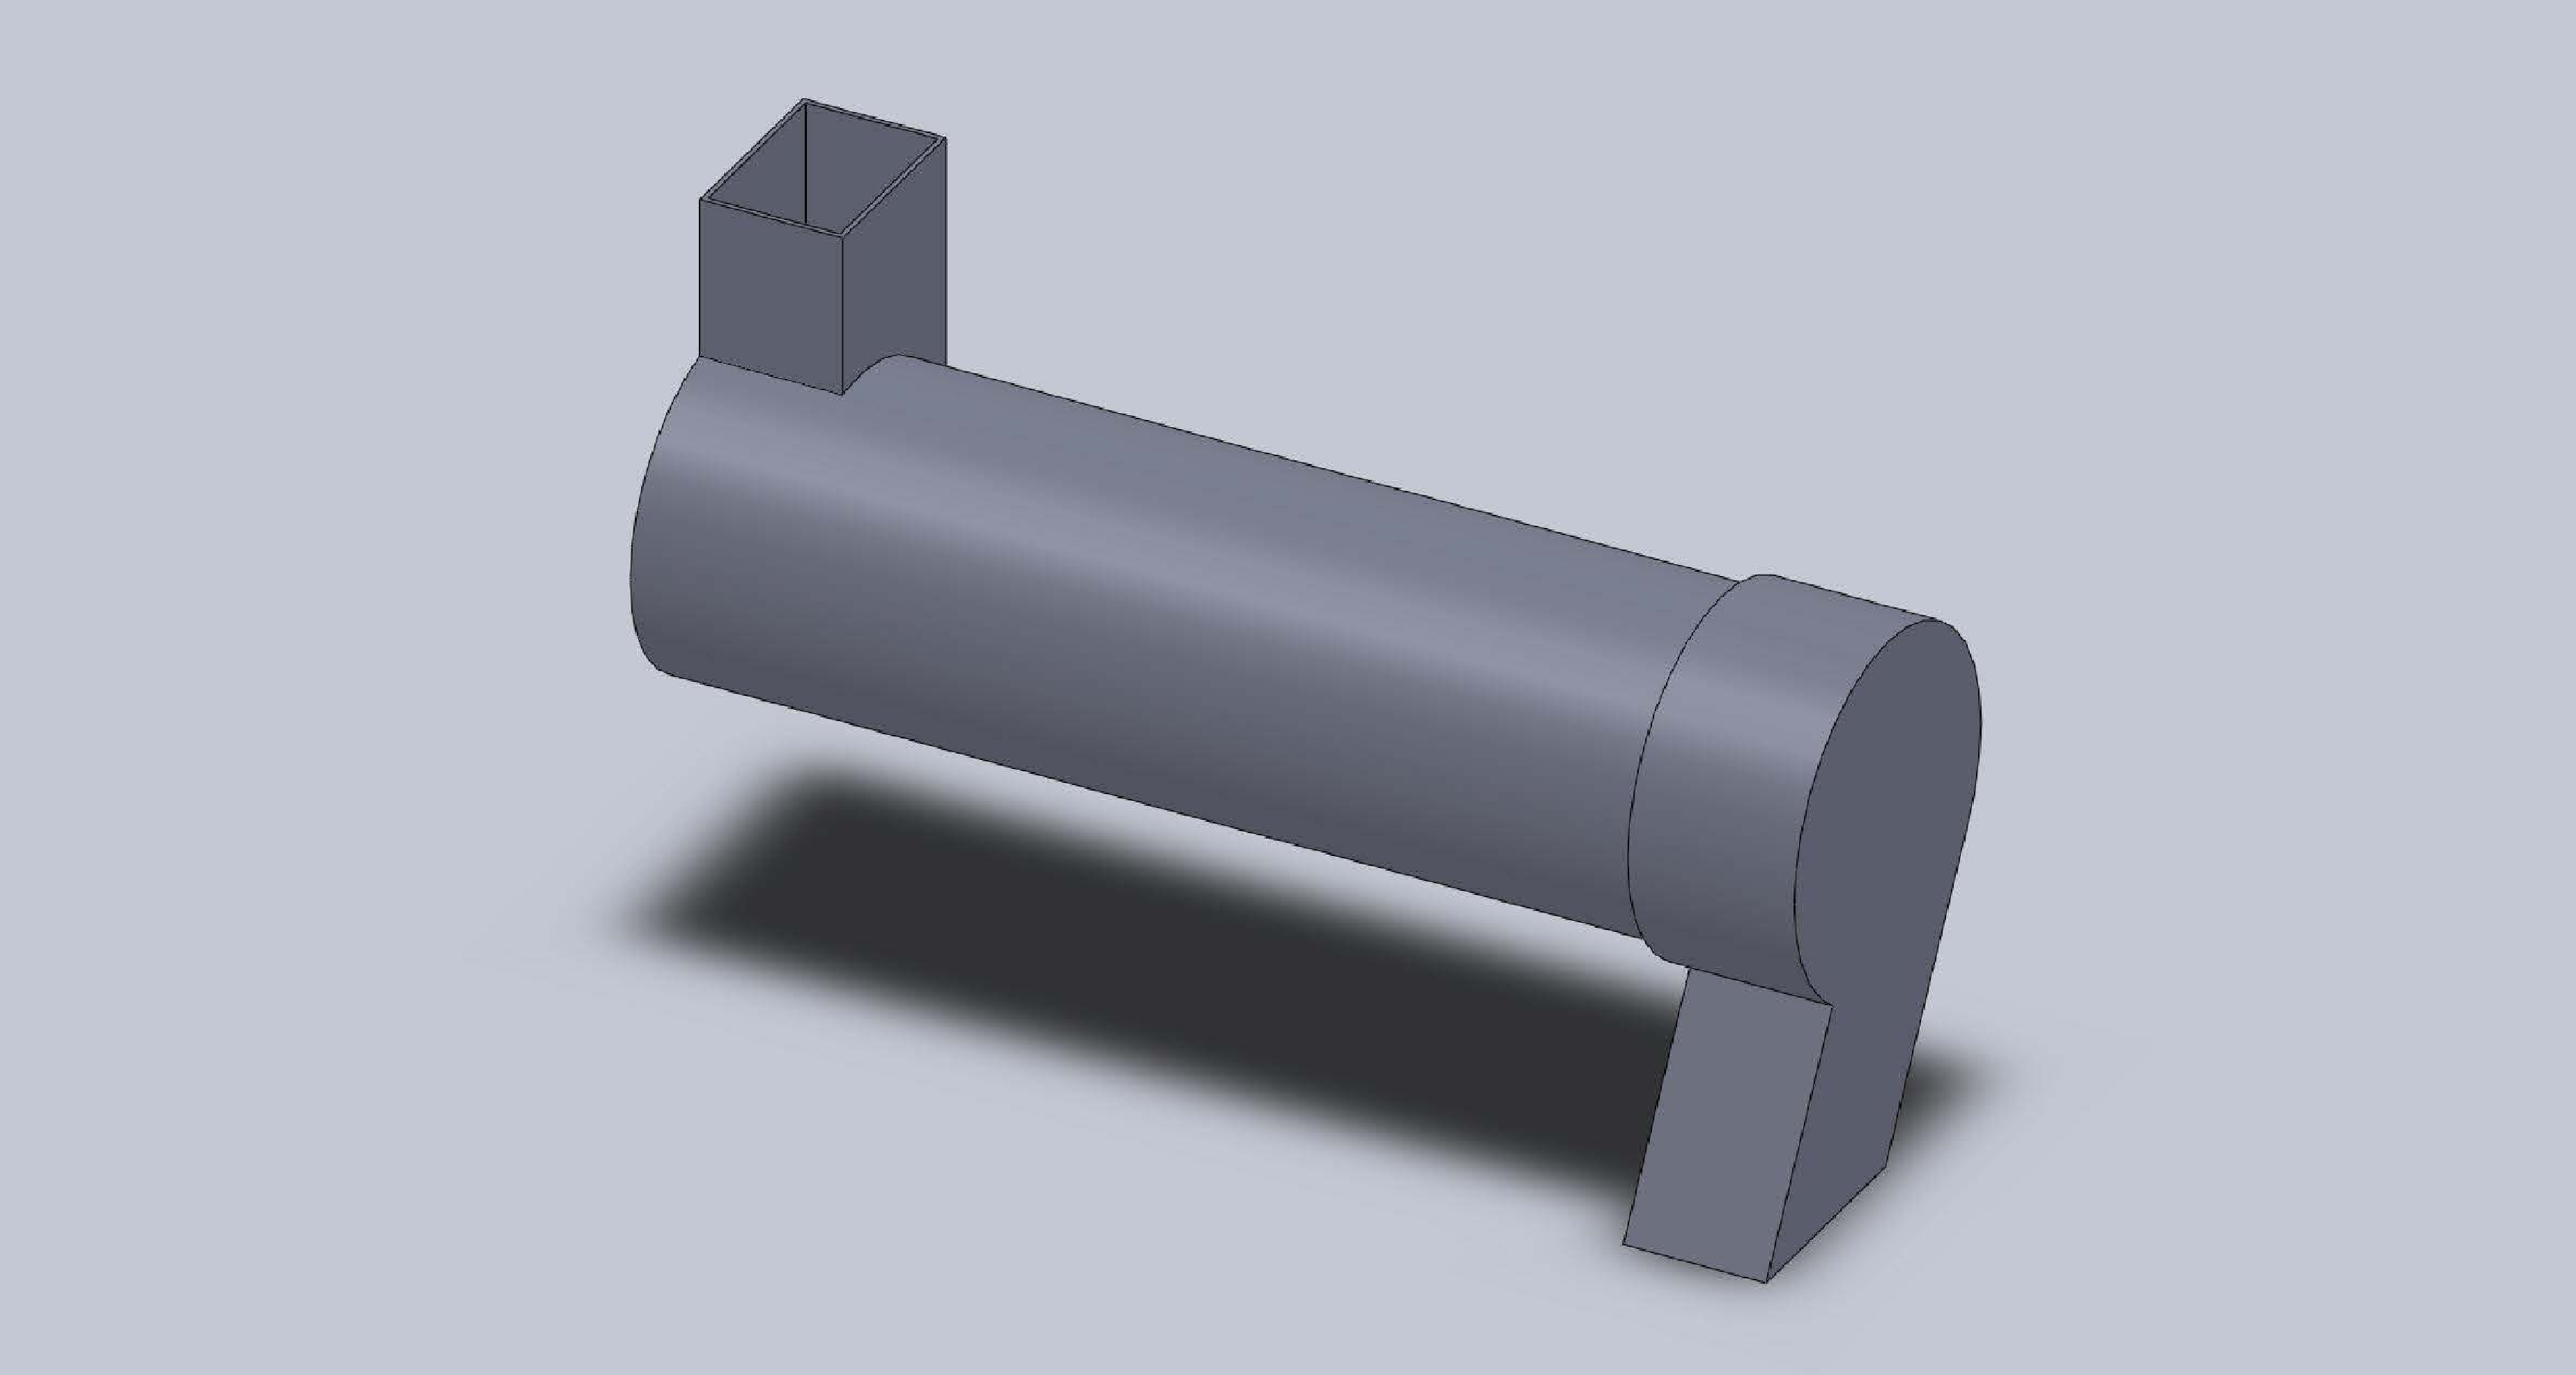
\includegraphics[scale=0.2]{shell_final_pic.pdf}
\caption{ Shows an isometric view of the granulator casing.}
\label{fig:mthdsDemCharlesGranShell}
\end{figure}

  The impeller consists of a cylindrical shaft of length 370 mm and diameter 68 mm with four 
flattened sides 15 mm wide running along the axis. The blades are placed on these flattened sides as 
shown in figure \ref{fig:mthds_dem_charles_impeller}. There are three different blade elements on the 
shaft (Figure \ref{fig:mthds_dem_charles_impeller}). At the granulator inlet, there are 4 paddle shaped 
feed elements following which there are 20 tear drop shaped shearing elements  and finally 4 
trapezoidal blades near the exit. All these elements are placed in a spiral configuration. The final 
configuration of the granulator is shown in Figure 
\ref{fig:mthds_dem_charles_fig5pt3and4_blades_n_isometric}.

\begin{figure}[H]
\centering
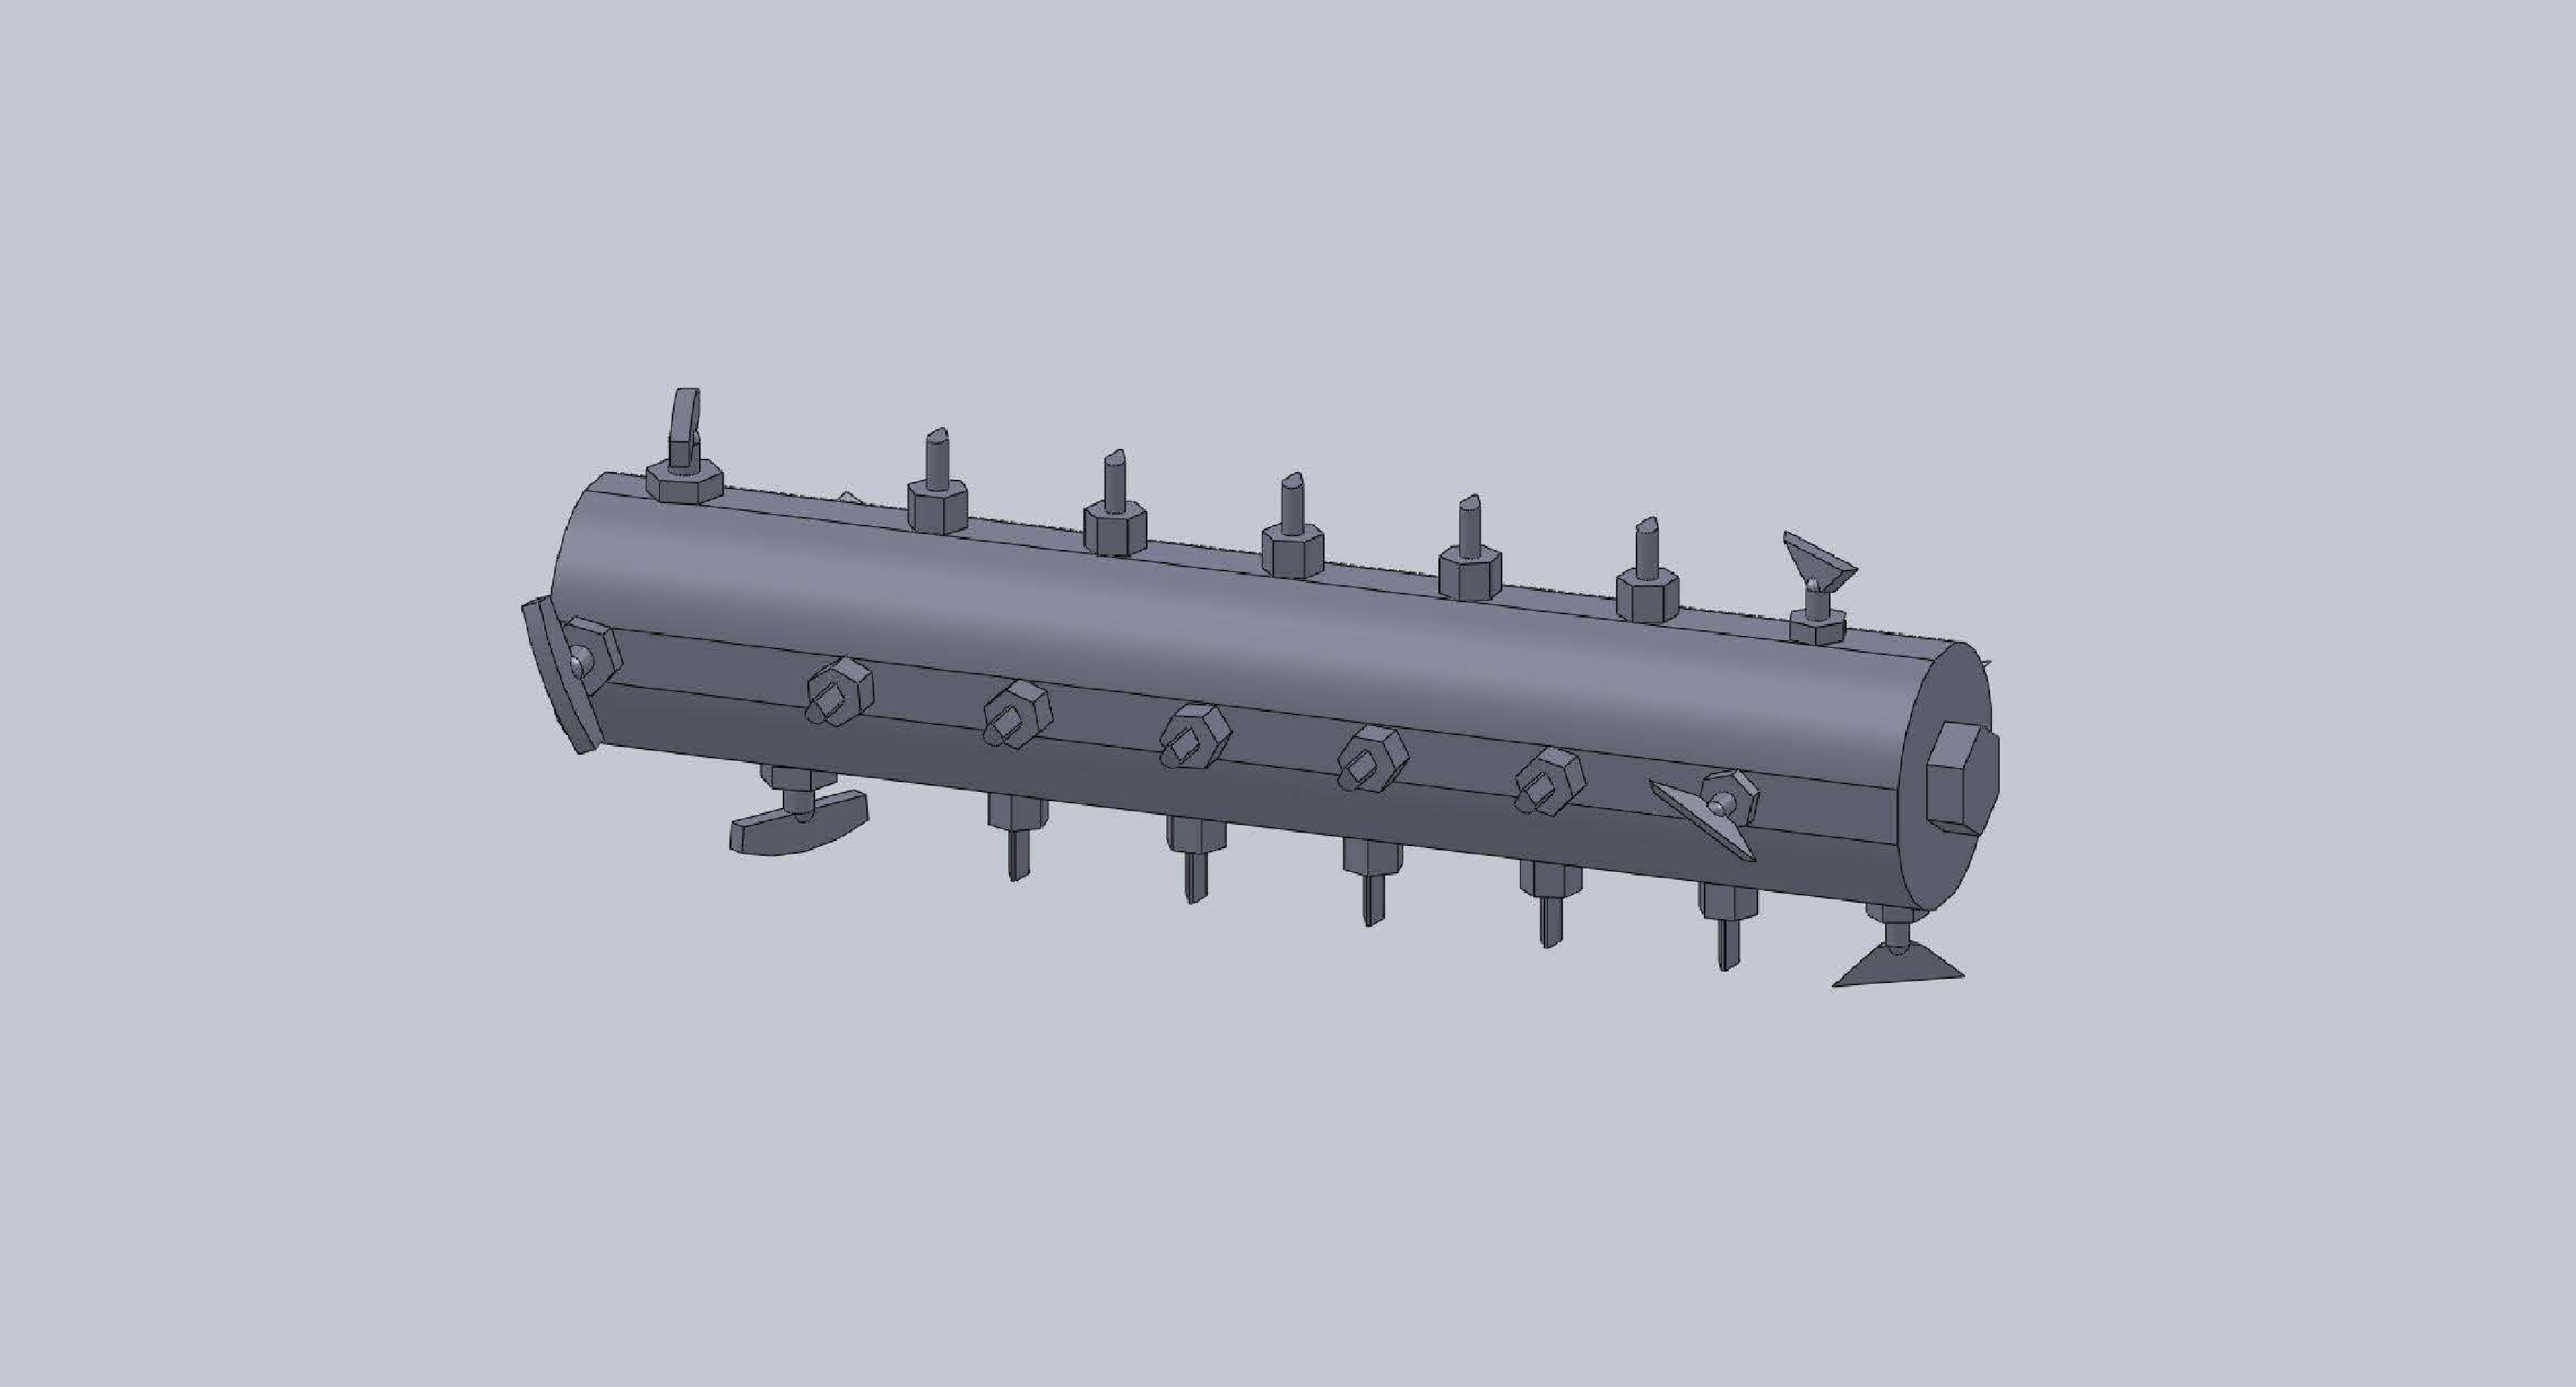
\includegraphics[scale=0.2]{impeller_final_pic.pdf}
\caption{This shows the isometric view of the impeller inisde the casing.}
\label{fig:mthds_dem_charles_impeller}
\end{figure}    

\begin{figure}[H]
\begin{subfigure}{.3\textwidth}
\centering
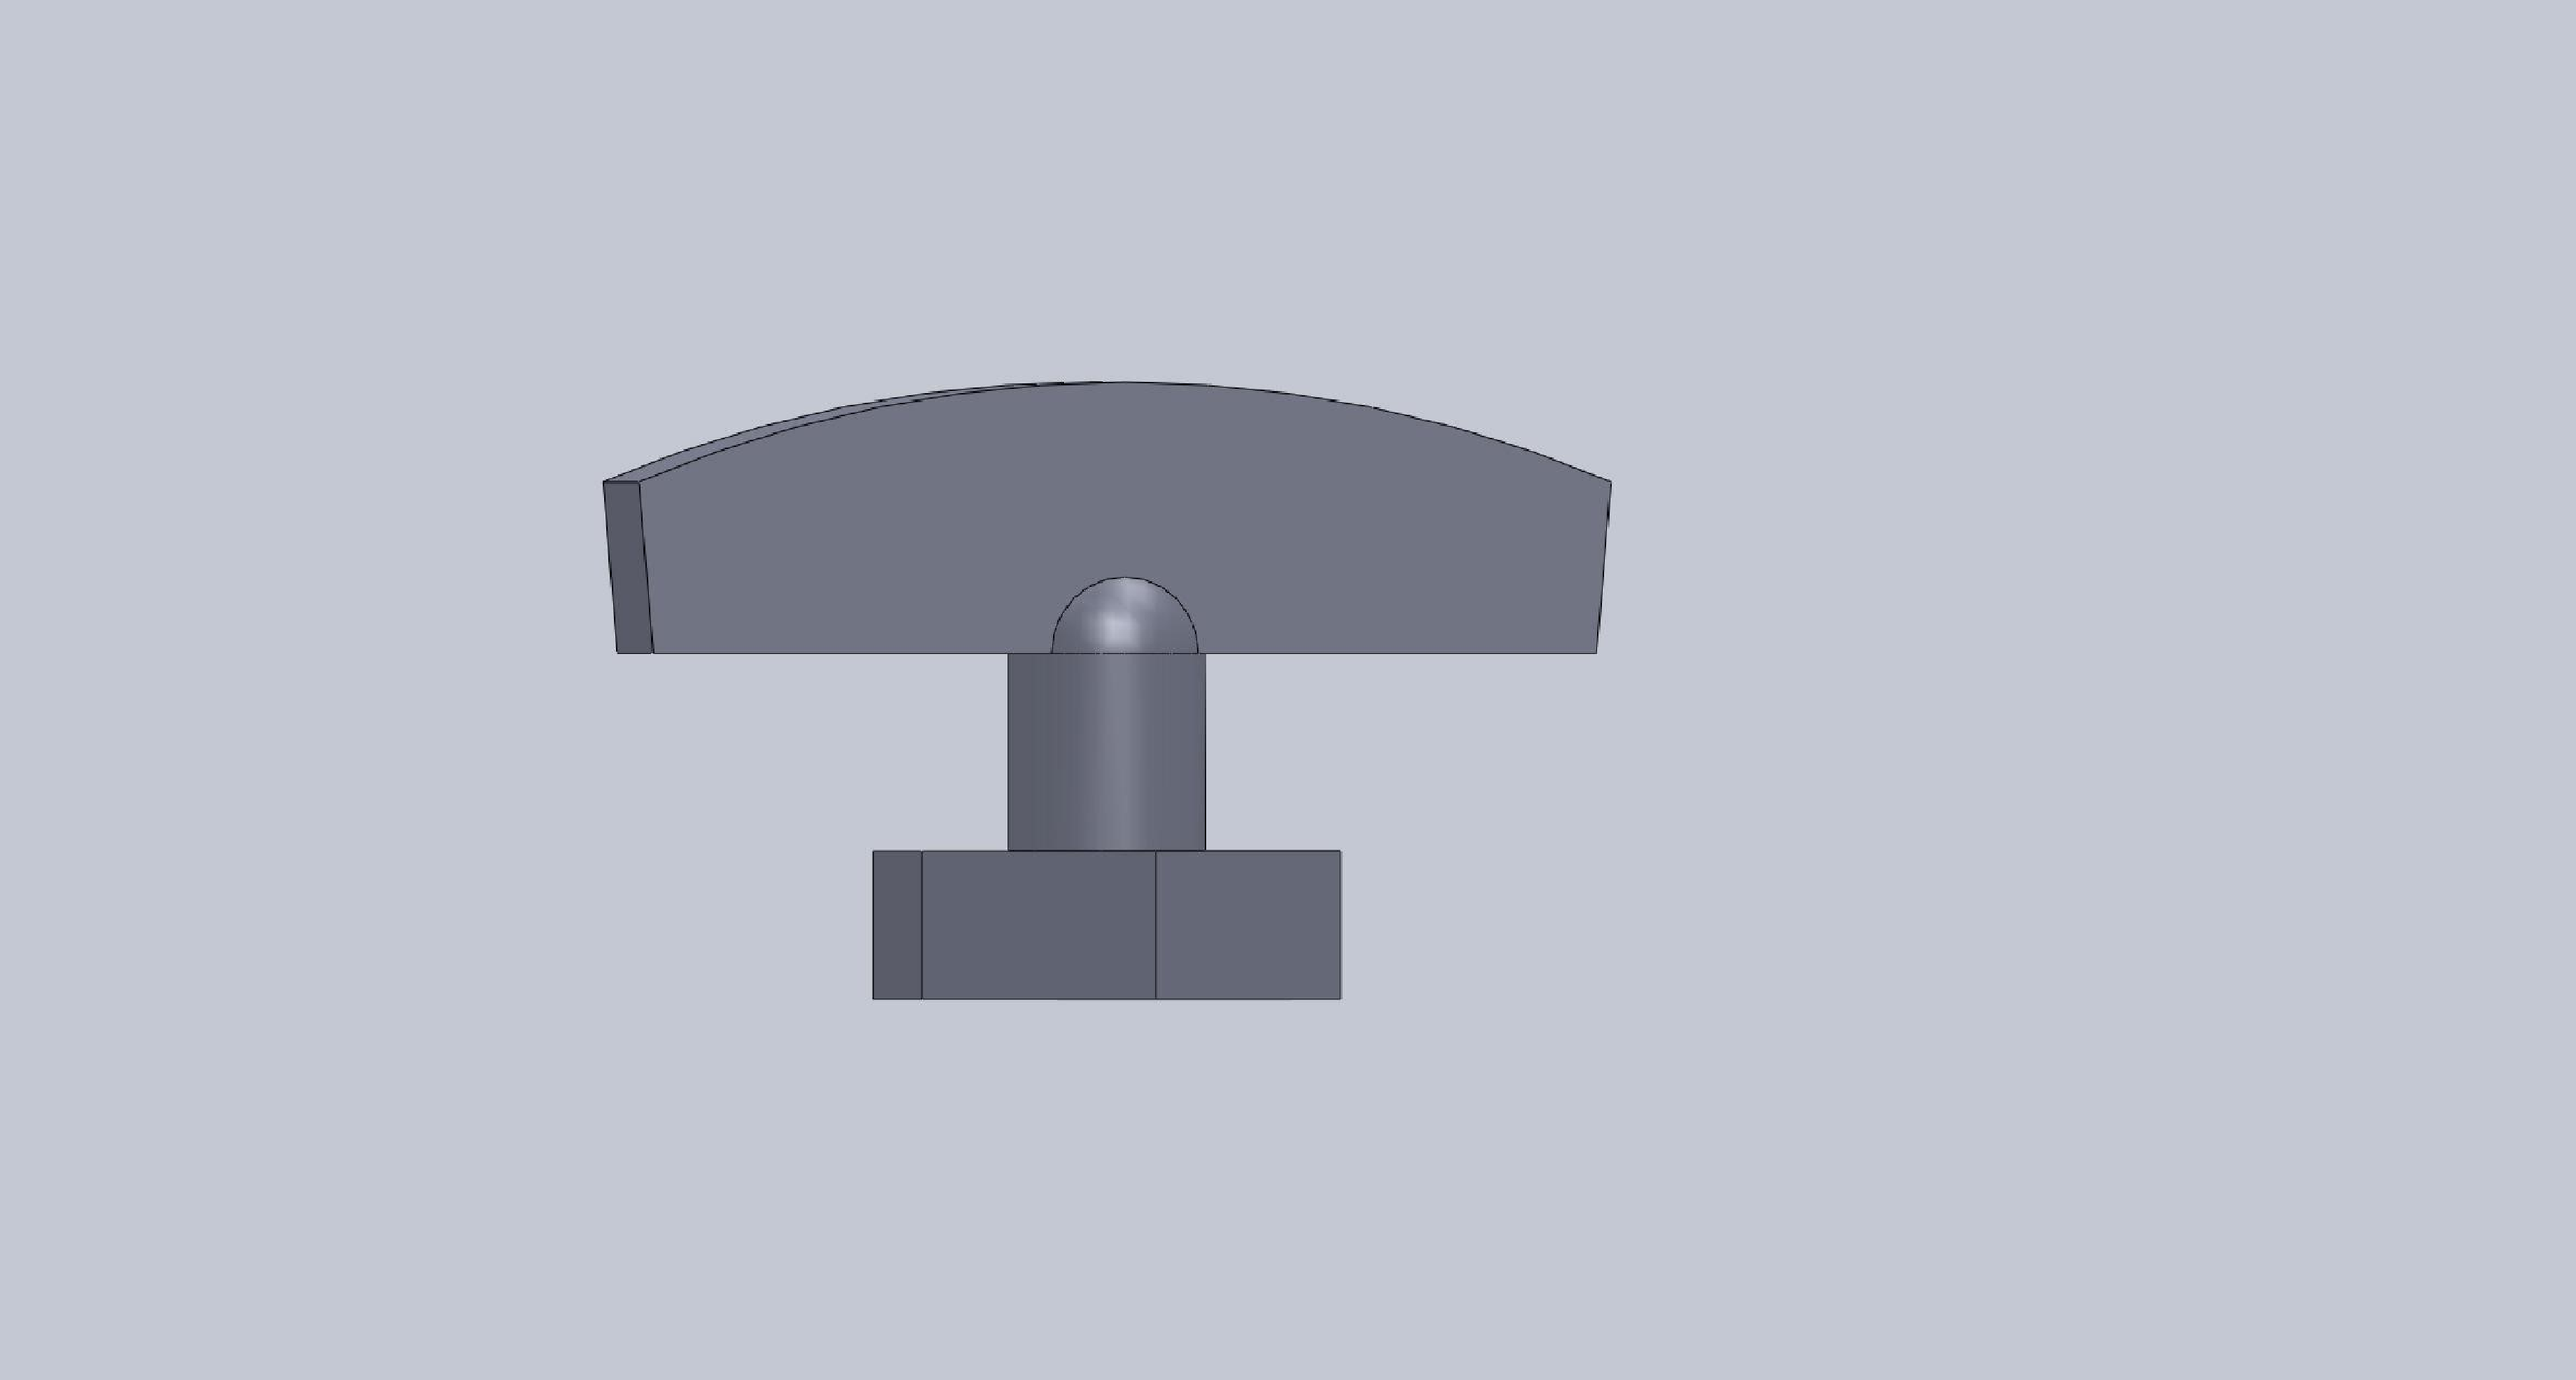
\includegraphics[scale=0.075]{feed_element.pdf}	      
\caption{Feed element}
\label{fig:mthds_dem_feed_element}
\end{subfigure}%
\begin{subfigure}{.3\textwidth}
	\centering
	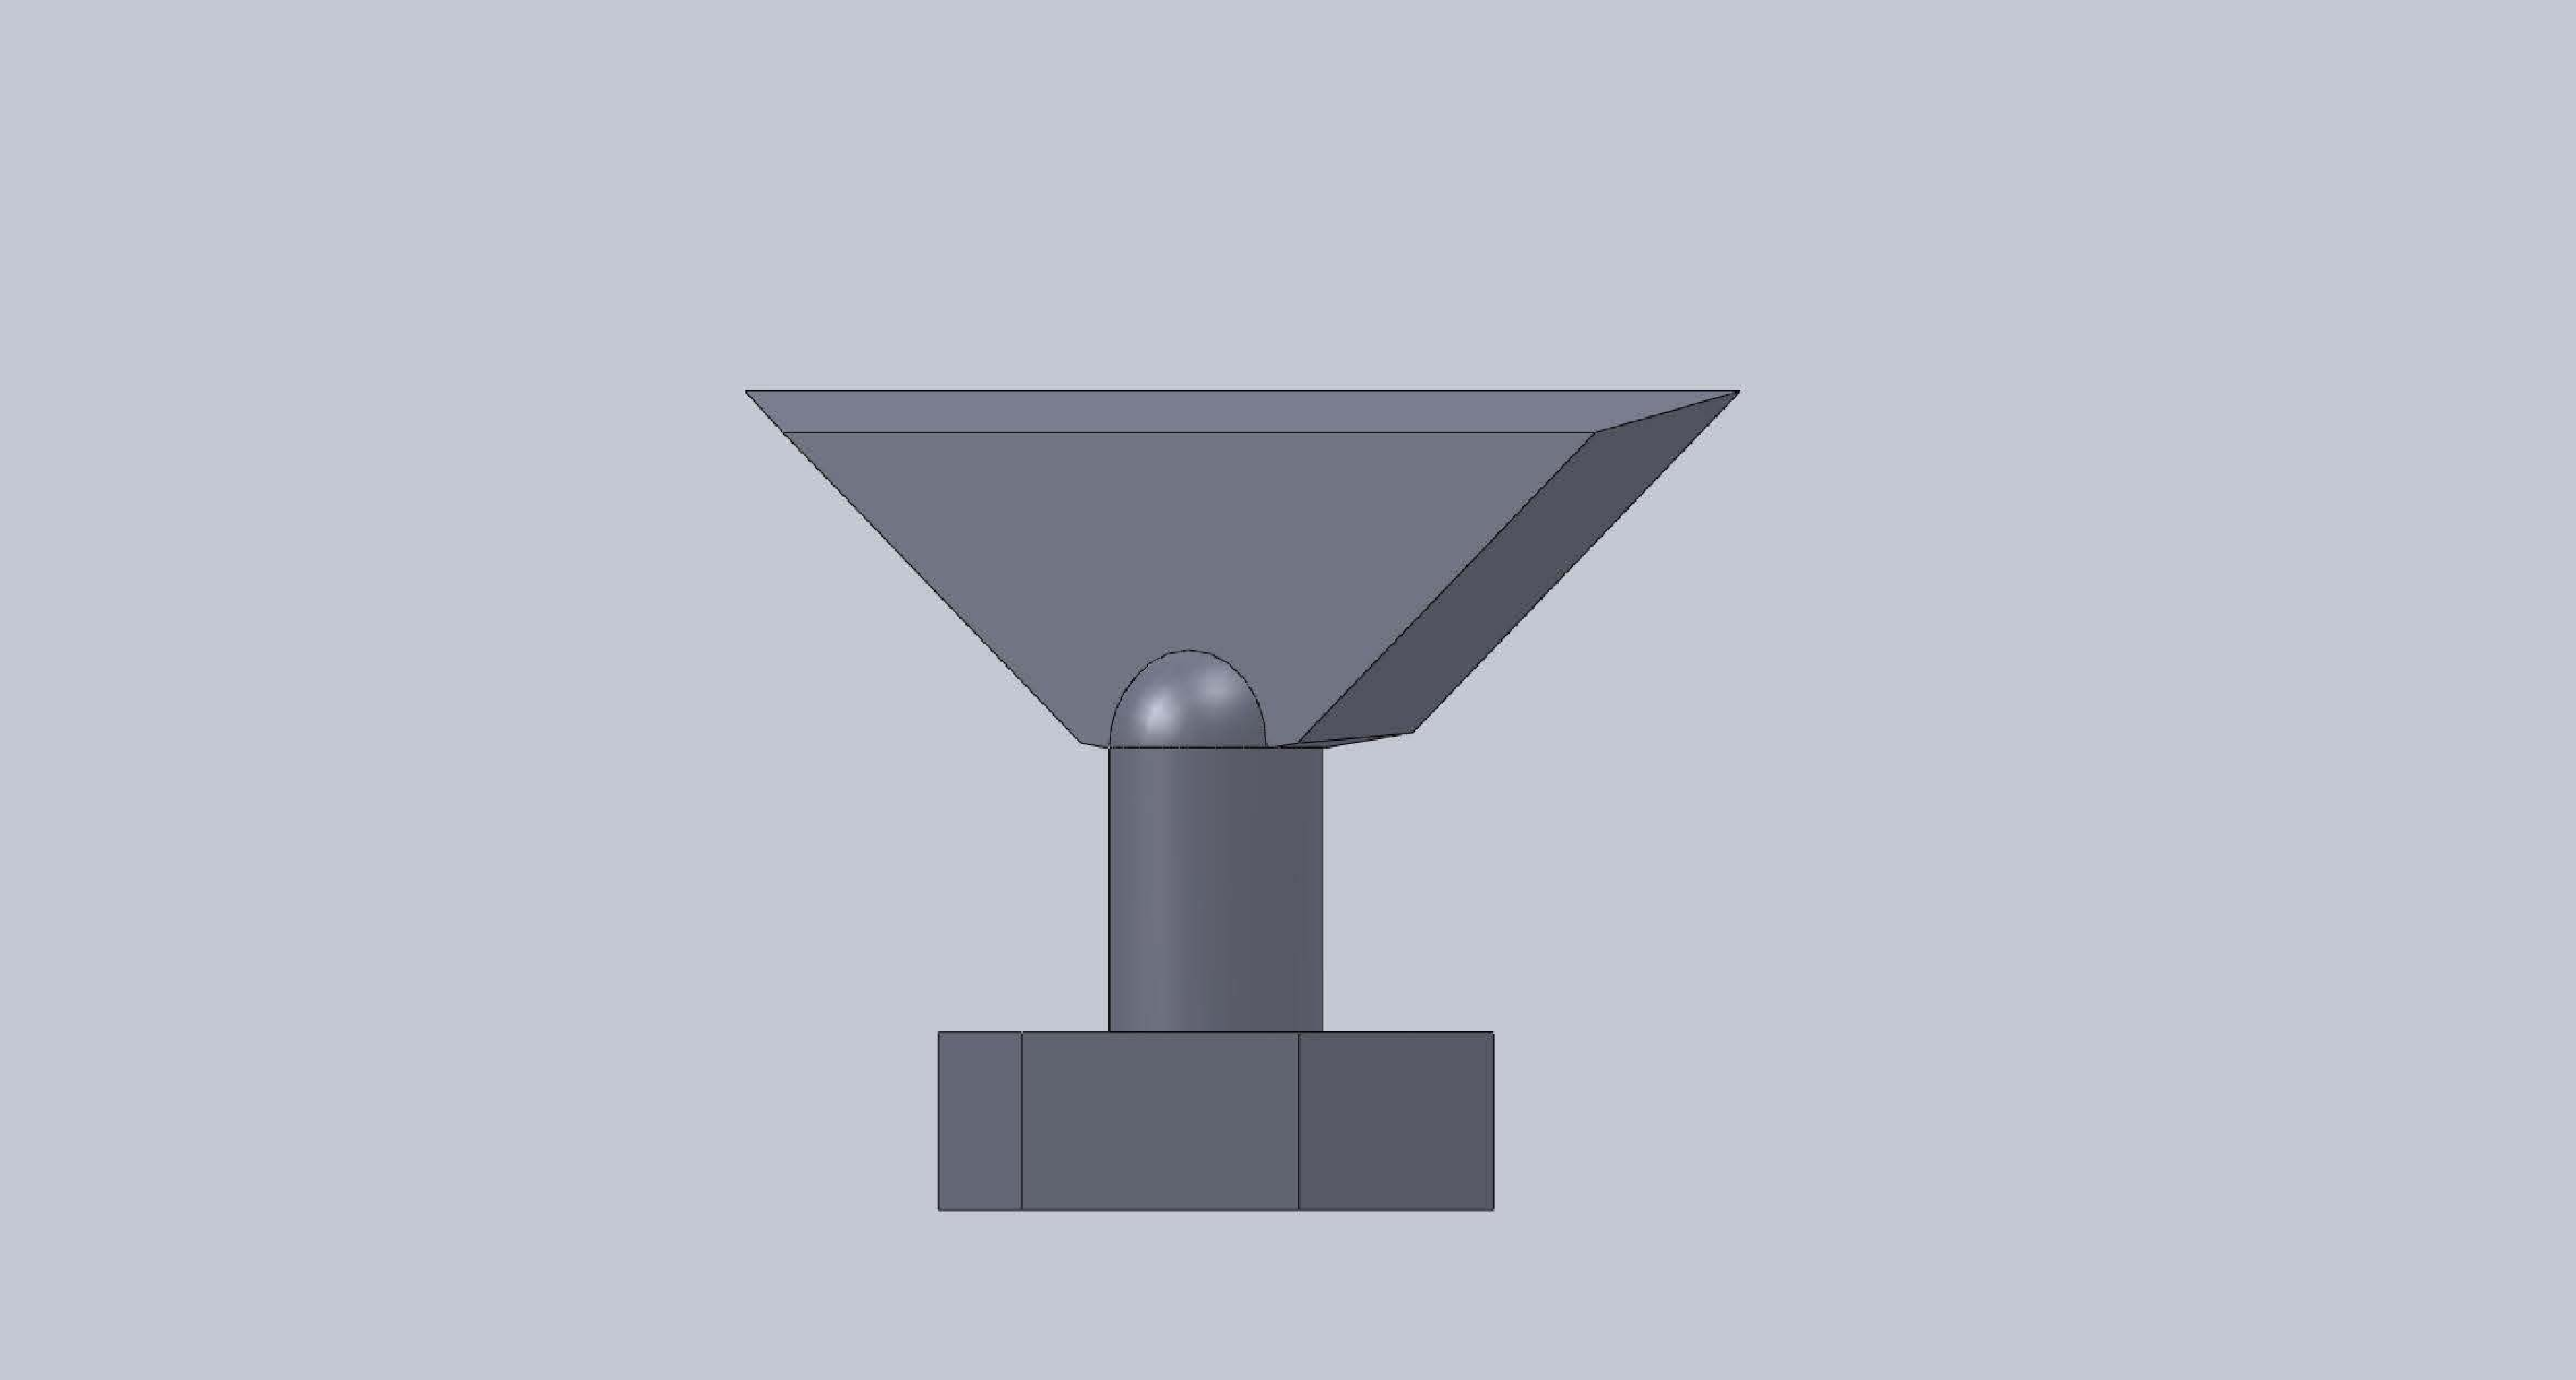
\includegraphics[scale=0.075]{exit_element.pdf}
	\caption{Exit element}
	\label{fig:mthds_dem_exit_element}
\end{subfigure}
\begin{subfigure}{.3\textwidth}
\centering
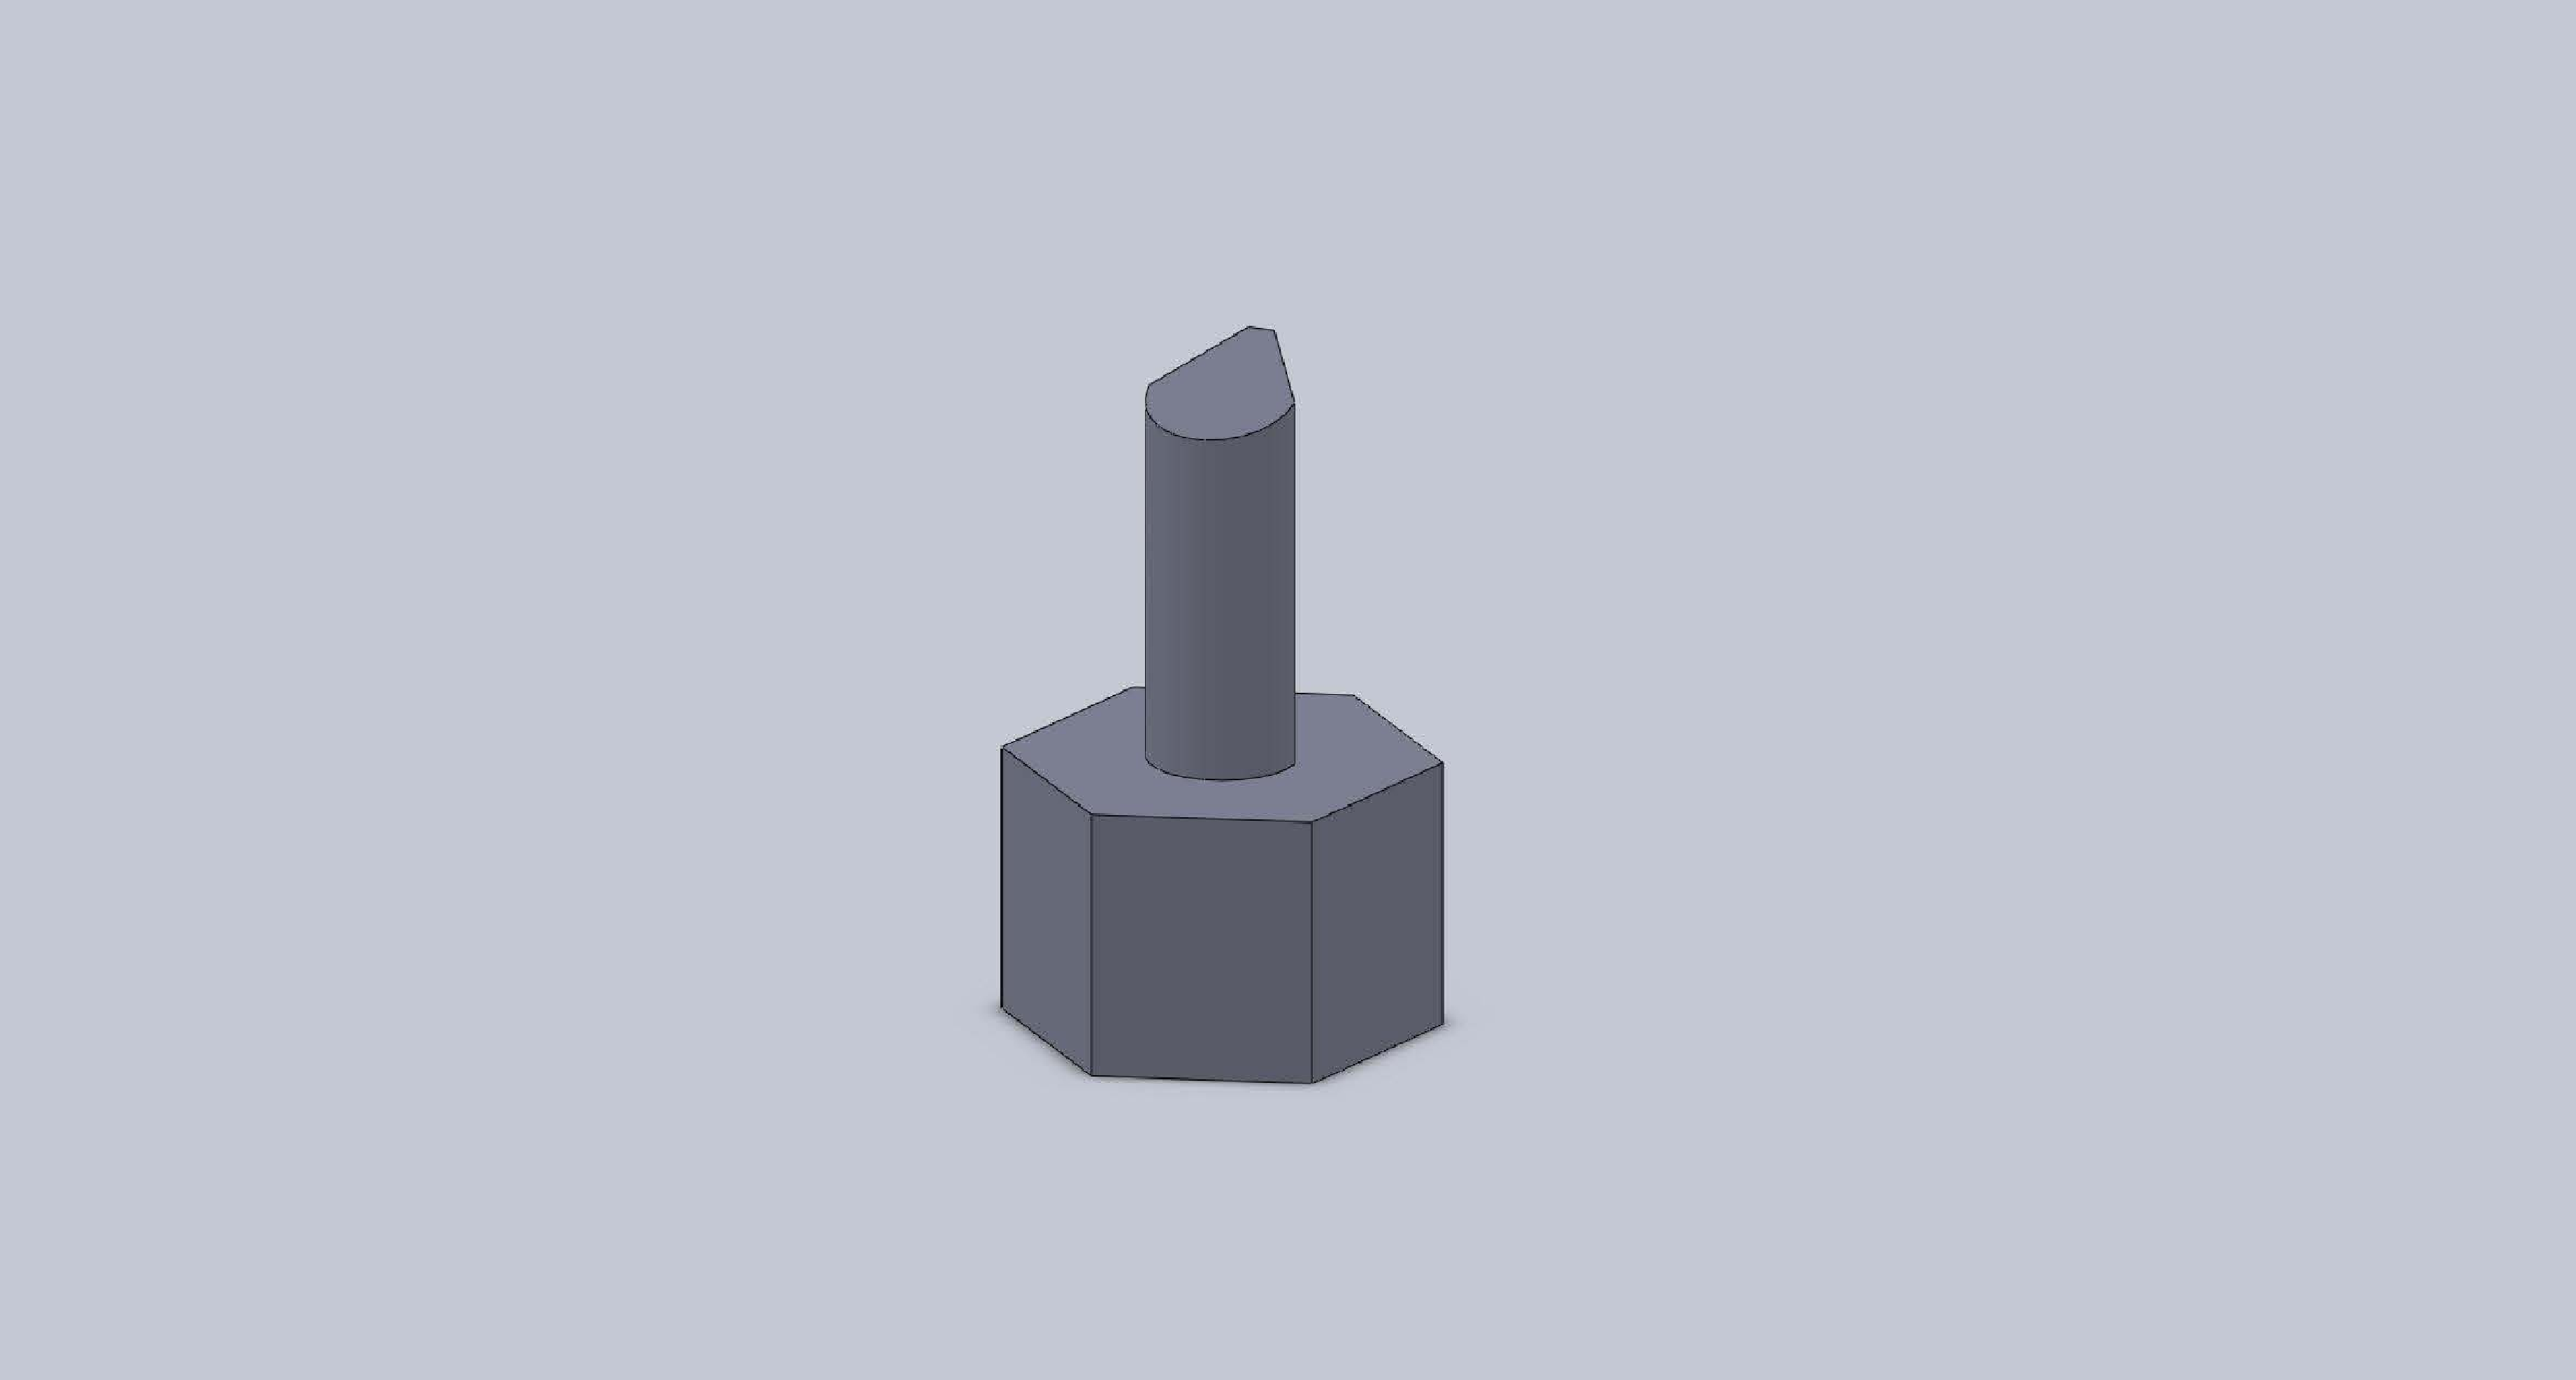
\includegraphics[scale=0.075]{shear_element.pdf}
\caption{Shear element}
\label{fig:mthds_dem_shear_element}
\end{subfigure}
\caption{Components (\subref{fig:mthds_dem_feed_element}) and (\subref{fig:mthds_dem_exit_element}) help in 
movement of the particles while (\subref{fig:mthds_dem_shear_element}) aids to throw the partilces to the wall 
inside the granulator.}
\label{fig:mthds_dem_charles_fig5pt3and4_blades_n_isometric}
\end{figure}     




\subsubsection{Meshing}
 After the geometry was built in SolidWorks$^{TM}$ (Dassault Syst\`{e}mes) the shell and impeller 
were exported as stereolithography (STL) files. The coarsest output option was used to keep the STL files small and 
simple for faster computations times. They were also exported not keeping there original coordinates.  
This resulted in the impeller having 2802 faces and 1281 points with approximately a file size of 775 
kilobytes. The shell had 1948 faces and 720 points and size was about 544 kilobytes.  
 Meshlab was used to align the STL files for importing into LIGGGHTS. No mesh treatments were 
used on the STLs. 
 The meshes were then imported into LIGGGHTS using the write command in serial. This resulted 
in 50 elements of the impeller file having "highly skewed elements", which have more than 5 
neighbours per surface or have an angle less than 0.0181185 degree, that according to LIGGGHTS 
would degrade parallel performance. The write exclusion list command in LIGGGHTS was used and 
this exclusion list file as then used in the simulation to skip the highly skewed elements during the 
simulation. 
%The shell did not have any skewed elements \textcolor{cyan}{(FUTURE SOLUTION? - perhaps we 
%can use the output from liggghts exclusion list to find exact elements of issue. then we can use 
%meshlab to exclude those peices or remesh thos individual pieces into better shapes with less 
%skewed elements. might be better for a letter paper though}

\subsubsection{DEM input file settings}
 The DEM simulation in LIGGGHTS are setup using an input script which defines the physical 
parameters of the particles, importing of the geometry, particle insertion commands, various physics 
models to be used during the simulation as well as various compute and dump commands to help print 
the data required for post-processing of the data. The particles were considered to be granular in 
nature. The Hertzian model was used for non-adhesive elastic contact between the granular particles. 
The particles were inserted inside the granulator from the inlet at a constant mass flow rate of 15 
kilograms per hour. The rotation speed of the impeller was kept throughout the study at 2000 rotations 
per minute. Such a high rotation speed was chosen since this would lead to high shear between the 
particles and the walls of the shell resulting in better size control of the granules. There were 2 sets of 
simulations that were performed, one with mono-sized particles and second consisting of a distribution 
of sizes. The particle radii chosen for mono-sized simulation varied 0.59mm - 2mm, consecutive 
particles radii had volume twice of one before them. The radii range of the distributed size simulation 
was 1mm - 3mm. The difference in the mechanics of these two simulations is discussed in the Section \ref{sec:Results}. 
The physical constants used for the simulations are given in Table 
\ref{table:mthds_dem_input}.
 The simulation data was collected after ever 50,000 time steps (5$\times 10^{-3}$ sec) 
for the visualization of the particles inside the shell, further post processing . The collisions 
between each of the particles and the collisions between of the particle and the geometry was 
collected and used in the PBM. 

\begin{table}[!htb]%[H]
\caption{Physical Properties of the particle for the LIGGGHTS input script} 
\label{table:mthds_dem_input}
\begin{center}
\begin{tabular}{l|c|c}
\hline
\bf{Parameter} &\bf{Value} &\bf{Units}\\
\hline
Young's Modulus of particles  & $8 \times 10^{6}$ & $N.m^{-2}$\\
Young's Modulus of Geometry  & $1 \times 10^{9}$ & $N.m^{-2}$\\
Poisson's Ratio & $0.2$ & $-$\\
Coefficient of restitution (constant for all collisions) & $0.4$ & $-$\\
Coefficient of static friction & $0.5$ & $-$\\
Coefficient of rolling friction  & $0.2$ & $-$\\
Density of the granules & $500$ & $kg.m^{-3}$\\
\hline
\end{tabular}
\end{center}
\end{table}

\subsubsection{DEM data post processing}
 The post processing of the data obtained from the DEM simulations was done using MATLAB. 
The first test run on the output data was to determine if the simulation had reached steady-state. The 
mass inside the granulator was found out by averaging it over 5 time steps and then compared to 
mass inside the granulator after every 10000 time steps (about 5$\times 10^{-4}$ sec) with a 
tolerance of about 10\%. If the mass was found to be constant for most of the iterations, it was 
considered to be at steady state. Another test to determine steady state was to monitor the number of 
collision inside the granulator. The visualization of the simulation data was done by running the 
LIGGHTS post processing (LPP) script over the dump files to convert them into STL files. These 
files were then loaded in to Paraview~\citep{henderson2004} for a graphical representation of the 
simulation. It can be seen that the number of collision start to oscillate around a mean value. The 
number of collisions were then plotted and steady state time was determined.
A precautionary script was also run so as to determine that no particles were lost due to overlap 
of the geometry with the particles as well as from particle particle overlap.


\subsection{PBM}
\label{sec:pbm_model}
\subsubsection{Model development}
 The population balance equation used in this work is expressed below:
\begin{align}
\frac{d}{dt}F(s_1,s_2,x)=\Re_{agg}(s_1,s_2,x)+\Re_{break}(s_1,s_2,x)+\dot{F}_{in}(s_1,s_2,x)-\dot{F}_{out}(s_1,s_2,x)
\label{eqn:mthds_pbm_overall} 
\end{align}
where, $F(s_1,s_2,x)$ is the number of particles with an active pharmaceutical ingredients (API) volume of $s_1$ and an excipient 
volume of $s_2$ in the spatial compartment $x$. The rate of change of number of particles with time 
in different size classes depend on the rate of aggregation $\Re_{agg}(s_1,s_2,x)$ and the rate of 
breakage $\Re_{break}(s_1,s_2,x)$. Also, the rate of particles coming into, $\dot{F}_{in}(s_1,s_2,x)$ and 
going out, $\dot{F}_{out}(s_1,s_2,x)$ of the spatial compartment due to particle transfer affect the number of 
particles in different size classes. 
The rate of change of liquid volume in each particle is calculated using the equation: 

\begin{align}
\frac{d}{dt}F(s_1,s_2,x)l(s_1,s_2,x)&= 
\Re_{liq,agg}(s_1,s_2,x)+\Re_{liq,break}(s_1,s_2,x)+\dot{F}_{in}(s_1,s_2,x)l_{in}(s_1,s_2,x)\notag\\
&-\dot{F}_{out}(s_1,s_2,x)l_{out}(s_1,s_2,x)+F(s_1,s_2,x)\dot{l}_{add}(s_1,s_2,x)
\label{eqn:mthds_pbm_rate} 
\end{align}

where, $l(s_1,s_2,x)$ is the amount of liquid volume in each particle with API volume of $s_1$ and 
excipient volume of $s_2$ in the spatial compartment $x$. $\Re_{liq,agg}(s_1,s_2,x)$ and 
$\Re_{liq,break}(s_1,s_2,x)$ are respectively the rates of liquid transferred between size classes due to 
aggregation and breakage. $l_{in}(s_1,s_2,x)$ and $l_{out}(s_1,s_2,x)$ are respectively the liquid 
volumes of the particles coming in and going out of the spatial compartment. $l_{add}(s_1,s_2,x)$ is 
the volume of liquid acquired by each particle in the compartment at every time step due to external 
liquid addition.
Similarly, the rate of change of gas volume is calculated using the following equation: 

\begin{align}
\frac{d}{dt}F(s_1,s_2,x)g(s_1,s_2,x)&= 
\Re_{gas,agg}(s_1,s_2,x)+\Re_{gas,break}(s_1,s_2,x)+\dot{F}_{in}(s_1,s_2,x)g_{in}(s_1,s_2,x)\notag\\
&-\dot{F}_{out}(s_1,s_2,x)g_{out}(s_1,s_2,x)+F(s_1,s_2,x)\dot{g}_{cons}(s_1,s_2,x)
\label{eqn:mthds_pbm_gas_agg} 
\end{align}

where, $g(s_1,s_2,x)$ is the gas volume of each particle with API volume of $s_1$ and excipient 
volume of $s_2$ in the spatial compartment $x$. $\Re_{gas,agg}(s_1,s_2,x)$ and 
$\Re_{gas,break}(s_1,s_2,x)$ are respectively the rates of gas transferred between size classes due to 
aggregation and breakage. $g_{in}(s_1,s_2,x)$ and $g_{out}(s_1,s_2,x)$ are respectively the gas 
volume of the particles entering and leaving the spatial compartment. $\dot{g}_{cons}(s_1,s_2,x)$ is the 
volume of gas coming out of each particle at every time-step due to consolidation of the particles. 
The rate of aggregation, $\Re_{agg}(s_1,s_2,x)$ in Equation \ref{eqn:mthds_pbm_overall} is 
calculated as: \citep{Chaturbedi2017}

\begin{align}
\Re_{agg}(s_1,s_2,x)&= \frac{1}{2}\int _0^{s_1} \int_0^{s_2} 
\beta(s_1',s_2',s_1-s_1',s_2-s_2',x)F(s_1',s_2',x)F(s_1-s_1',s_2-s_2',x)ds_1'ds_2'\notag\\ 
&- F(s_1,s_2,x)\int _0^{s_{max_1}-s_1} \int_0^{s_{max_2}-s_2} 
\beta(s_1,s_2,s_1',s_2',x)F(s_1',s_2',x)ds_1'ds_2'
\end{align}


where, the aggregation kernel, $\beta(s_1,s_2, s_1',s_2',x)$ is expressed as a function of collision 
rate coefficient ($C$) and probability that collision results in agglomeration($\psi$) \citep{ingram2005}
and is shown below: 

\begin{align}
\beta(s_1,s_2,s_1',s_2',x) = \beta_oC(s_1,s_2,s_1',s_2',x)\psi(s_1,s_2,s_1',s_2',x)
%\beta(s_1,s_2,s_1',s_2',x) = & \beta_o*(V(s_1,s_2,x)+V(s_1',s_2',x))^{\gamma}*(c(s_1,s_2,x)\notag\\
%&+c(s_1',s_2',x))^{\alpha}\left(1-\frac{(c(s_1,s_2,x)+c(s_1',s_2',x))^{\delta}}{2}\right)^{\alpha}
\label{eqn:mthds_pbm_beta_kernal}
\end{align}

where, $\beta_o$ is aggregation rate constant.\\
Collision rate coefficient ($C$) is a function of particle sizes and is calculated by normalizing the 
number of collisions between group of particles \citep{gantt2006} and is obtained from LIGGGHTS 
DEM simulation. A recent study shows that collision frequency depends on PSD as well 
\citep{sen2014}. Collision rate coefficient can be expressed as:

\begin{align}
C(s_1,s_2,s_1',s_2')=\frac{N_{coll}(s_1,s_2,s_1',s_2')}{N_p(s_1,s_2)N_p(s_1',s_2')\Delta t}
\label{eqn:collfreq}
\end{align}

In Equation \ref{eqn:collfreq}, $N_{coll}$ is the number of collision between two particles in 
time interval $\Delta t$ \& $N_p$ is number of particle of particular size. The agglomeration 
($\psi$) in equation (\ref{eqn:mthds_pbm_beta_kernal}) can be expressed as:

\begin{align}
\psi((s_1,s_2,s_1',s_2') = 
\left\{\begin{matrix}
\psi_0,\hspace{0.2cm} LC((s_1,s_2) \geq LC_{min}\hspace{0.2cm} and\hspace{0.2cm} LC((s_1',s_2') \geq LC_{min}	\\ 
0,\hspace{0.2cm} LC((s_1,s_2) < LC_{min}\hspace{0.2cm} or\hspace{0.2cm} LC((s_1',s_2') < LC_{min}
\end{matrix}\right.
\label{eqn:colleff}
\end{align}
 In Equation \ref{eqn:colleff}, $LC$ is the liquid content of particles and $LC_{min}$ stands for minimum 
 liquid content required for coalescence of particles. 

%%%%% commented the breakage details as we aren't including in results


%	     Similarly, the breakage rate is expressed as-
%	
%	    \begin{align}
%	    \Re_{break}(s_1,s_2,x) = \int_0^{s_{max_1}} \int_0^{s_{max_2}} 
%K_{break}(s_1',s_2',x)F(s_1',s_2',x)ds_1'ds_2' - K_{break}(s_1,s_2,x)F(s_1,s_2,x)
%	    \end{align}
%%	     \textcolor{red}{citation?}
%	    
%	     where, the breakage kernel $K_{break}(s_1,s_2,x)$ is formulated as – 
%	    
%	    \begin{align}
%	    K_{break}(s_1,s_2,x) = C_{impact}\int_{U_{break}}^{\infty}p(U)dU
%	    
%K_{break}(s_1,s_2,x)=\left(\frac{4}{15\pi}\right)^{(\frac{1}{2})}G_{shear}exp\left(-\frac{B}{R(s_1,s_2,x)}\ri
%ght)
%	    \end{align}
%	     \textcolor{red}{citation?}

% where, $G_{shear}$ is the shear rate exerted by the impeller on the granules. $R(s_1,s_2,x)$ is 
%the radius of the granule that breaks and $B$ is the breakage kernel constant. $G_shear$ is 
%calculated as $\frac{\nu_{impeller}*D_{impeller}*PI}{60}$ where $\nu_{impeller}$ and $D_{impeller}$ 
%are respectively the rotational speed and diameter of the impeller.
The rate of increase of liquid volume of a particle, $\dot{l}_{add}(s_1,s_2,x)$ is expressed as:

\begin{align}
\dot{l}_{add}(s_1,s_2,x) = \frac{(s_1+s_2)(\dot{m}_{spray}(1-c_{binder})-\dot{m}_{evap})}{m_{solid}(x)}
\end{align}

where, $(s_1+s_2)$  is the total solid volume of the particle; $\dot{m}_spray$ is the rate of external 
liquid addition, $c_{binder}$ is the concentration of binder in the external liquid (which is assumed to 
be zero in this case); $\dot{m}_{evap}$ is the rate of evaporation of liquid from 
the system (which is also assumed to be zero in this case) and $m_{solid}$ is the total amount of solid 
present in the compartment.
The rate of decrease in gas volume per particle due to consolidation is calculated using the 
following expression: \citep{Verkoeijen2002} 

\begin{align}
\dot{g}_{cons}(s_1,s_2,x)=&c (\nu_{impeller})^{\omega}V(s_1,s_2,x)\frac{(1-\epsilon_{min})}{s} 
\notag \\ 
& \left[g(s_1,s_2,x)+l(s_1,s_2,x) -(s_1+s_2)\frac{\epsilon_{min}}{1-\epsilon_{min}}\right]
\end{align}        

 where, $c$ and $\omega$ are the consolidation constants; $v_{impeller}$ is the impeller 
rotational speed; $V(s_1,s_2,x)$ is the volume of particle, $\epsilon_{min}$ is the minimum porosity; 
$g(s_1,s_2,x)$ and $l(s_1,s_2,x)$ are respectively the gas and liquid volumes of the particle.

 Particle transfer rate, $\dot{F}_{out}(s_1,s_2,x)$ in Equation \ref{eqn:mthds_pbm_overall} is calculated 
as:

\begin{align}
\dot{F}_{out}(s_1,s_2,x) = \dot{F}(s_1,s_2,x)*\frac{\nu_{compartment}(x)*dt}{d_{compartment}}
\end{align}

where, $\nu_{compartment}(x)$ and $d_{compartment}$ are respectively the average velocity of 
particles in compartment $x$ and the distance between the mid-points of two adjacent compartment, 
which is the distance particles have to travel to move to the next spatial compartment. $dt$ is the 
time-step.
The values of various parameters used in the model are provided in Table 
\ref{table:mthds_pbm_parameters}.
\subsubsection{PBM parameters}
The process parameters and physical constants used in the PBM simulation are listed in Table 
\ref{table:mthds_pbm_parameters}.
\begin{table}[H]
\caption{Parameters for PBM}
\label{table:mthds_pbm_parameters}
\begin{center}
\begin{tabular}{l|c|c|c}
\hline
\bf{Parameter} &\bf{Symbol} &\bf{Value} &\bf{Units}\\
\hline
Time step & $\delta t$ & $0.5$ & $s$\\
Total granulation time & $T$ & $45, 45$ & $s$\\
Velocity in axial direction & $v_{axial}$ & $1$ & $ms^{-1}$\\
Velocity in radial direction & $v_{radial}$ & $1$ & $ms^{-1}$\\
Aggregation constant & $\beta_0$ & $1\times10^{-9}$ & $-$\\
Initial particle diameter & $R$ & $150$ & $\mu m$\\
Breakage kernel constant & $B$ & $0$ & $-$\\
Diameter of impeller & $D$ & $0.114$ & $m$ \\
Impeller rotation speed & $RPM$ & $2000$ & $rmp$\\
Minimum granule porosity & $\epsilon_{min}$ & $0.2$ & $-$\\
Consolidation rate & $C$ & $0$ & $-$\\
Total starting particles in batch & $F_{initial}$ & $1 \times 10^{6}$ & $-$\\
Liquid to solid ratio & $L/S$ & $0.35$ & $-$ \\
Number of Compartments & $c$ & $4$ & $-$ \\
Number of first solid bins & $s$ & $16$ & $-$\\
Number of second solid bins & $ss$ & $16$ & $-$\\
\hline
\end{tabular}
\end{center}
\end{table}


\subsection{PBM Parallel C++}
\subsubsection{Discretization \& parallelizing PBM}
 The PBM was discretized by converting each of its coordinates in to discrete bins. For the spatial 
coordinates a linear bin spacing was used. For the internal coordinates, solid, liquid and gas a 
non-linear discretization was used.
 Once the PBM had been discretized, a finite differences method was 
used which created a system of ordinary differential equations (ODEs) \citep{Barrasso2015cerd}. The 
numerical integration technique used to evaluate the system of ODEs was first order Euler integration 
as it is commonly used to solve these types of systems and author found an improvement in  speed while 
having minimal impact on accuracy \citep{Barrasso2013}. In order to avoid numerical instability due to the explicit nature of the Euler integration, Courant-Friedrichs-Lewis (CFL) condition must be satisfied~\citep{courant1967}. For our PBM model, time-step was calculated at each iteration such that, the number of particles leaving a particular bin at any time is less than the number of particles present at that time \citep{Ramachandran2010}. To obtain the most optimal parallel 
performance, when solving the PBM, work loads were distributed in a manner which took into account 
the shared and distributed memory aspects of the clusters, the PBM was being run on. To 
parallelize the model in a way which could take advantage of shared memory but still effectively run 
across a distributed system both MPI and OMP were implemented. 
 One MPI process was used per CPU socket and one OMP thread was used per CPU core, as 
authors (\cite{Bettencourt2017}) found it resulted in the best performance. MPI was used for message 
passing from one node to another while OMP was used for calculations on each node that could be 
efficiently solved using a shared memory system. 
 An algorithm in the form of pseudo code is presented below illustrating how the calculations are distributed and carried out 
during the simulation. For each time step, the MPI processes are made responsible for a specific chunk 
of the spatial compartments. Then each OMP thread, inside of each MPI process, is allocated to one of 
the cores of multi-core CPU the MPI process is bound too. The OMP threads divide up and 
compute $\Re_{agg}$. After $\Re_{agg}$ is calculated the MPI 
processes calculate the new PSD value for their chunk at that specific time step, $F_{t,c}$. The slave 
processes send their $F_{t,c}$ to the master processes which collects them into the complete 
$F_{t,all}$. The master process then broadcasts the $F_{t,all}$ value to all slave processes. This 
decomposition of the data into different CPUs and further into various threads is illustrated in Figure 
\ref{fig:mthds_PBM_decompostion}.	

\begin{figure}[H]
\centering
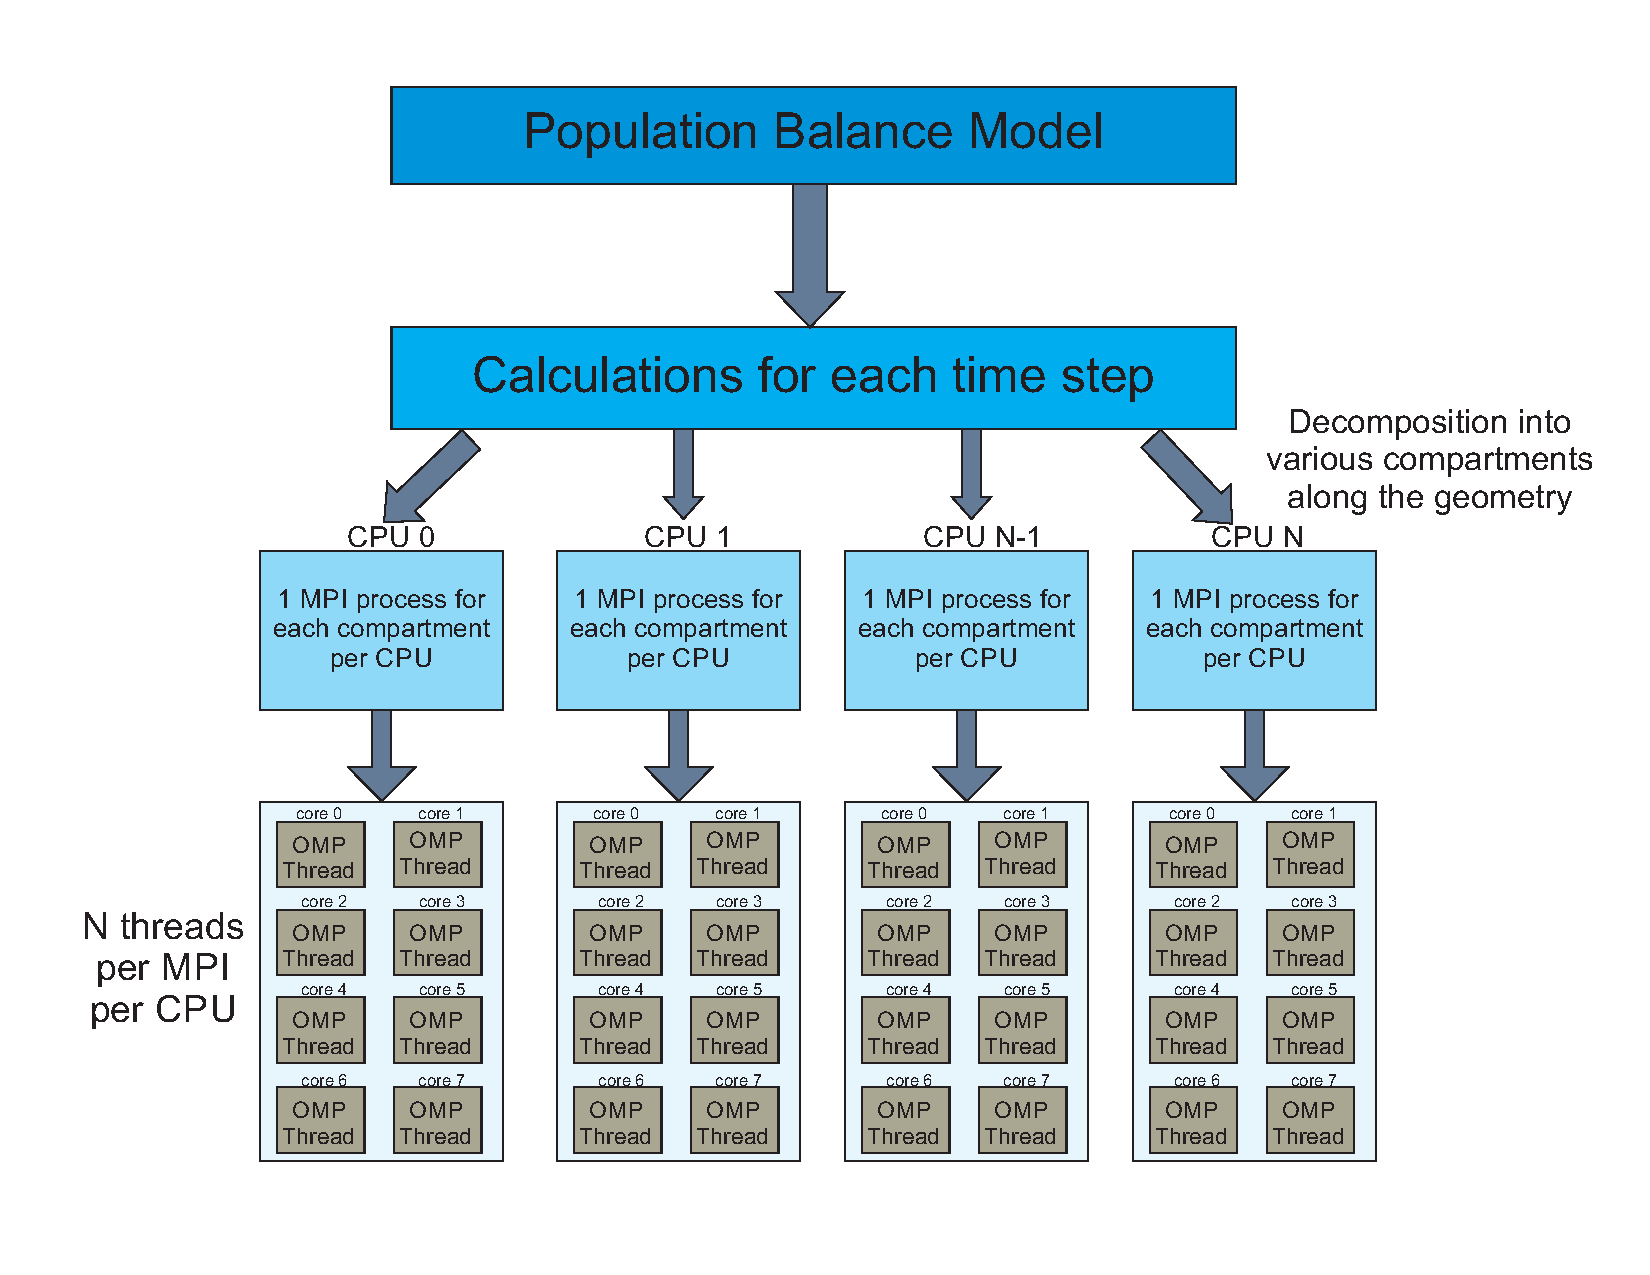
\includegraphics[scale=0.5]{PBM_decomposition.pdf}
\caption{The distribution of calculations using hybrid parallelization (MPI + OMP).}
\label{fig:mthds_PBM_decompostion}
\end{figure}

 A crucial feature of the PBM is that the current PSD ($F_{t,all}$) value is used to compute a new 
time step size for the next iteration. This means all of the MPI processes need to have the same 
dynamic time step size at each iteration for the calculations to be properly carried out in parallel. Since 
the completely updated $F_{t,all}$ value is shared before calculating a new time step each process will 
have the same $F_{t,all}$ value. As a result each process calculates the same size for the new time 
step. 
 Since the PBM code developed used the Standard Template Library containers and their features available in C++ 11 and later. It requires intel v15.0.2 or
later for compilation. Since this module was not present on the Stampede, the execution of the PBM was done on
the newer Stampede2 supercomputer. Each of the compute node of the cluster consists of Intel Xeon Phi 7250 
(\textquotedblleft Knights Landing\textquotedblright) which has 68 cores on a single socket clocked at 1.4 GHz, with 96 GB of DDR4 RAM. Each of 
the cores consists of 4 hardware threads. The simulations were then run by varying the the number of MPI 
processes from 1 to 16 and the number of OMP threads from 1 to 8, thus, using a maximum of 128 cores.
%\textcolor{cyan}{ Did not include the liquid and gas PBMs in this but hoping they will be some what 
%assumed? Also the Ragg omp distributed work is an a}
%\textcolor{red}{what about private OMP vars specified that has impact on how model is solved etc. 
%Should look into this. might change based on locking/blocking tests that need to be implemented 
%still.}   

\begin{algorithm}[!h]
\caption*{\textbf{Pseudo Code}}
\label{alg:MyAlgorithm}
\begin{algorithmic}[*]
\While{ $t<t_{final}$ }
\par // the spatial domain is divided into equal chunks (with in 1 bin size)
\par // each MPI process is assigned on chunk of spatial domain shown as $c_{low}$ to $c_{up}$ 
\par // sum all $c_{low_i}$ to $c_{up_i}$ is = to [0,numCompartments]

\For{each MPI processes} $c = c_{low_i}$ to $c_{up_i}$
\par   // each MPI process is further divided with OMP to take advantage of multi-core CPU
\par   // each OMP process is allocated to a single compute core
\par   // $\Re$ integrals $(i1)$ $\int_{0}^{s_2}$, $(i2)$ $\int_{0}^{s_{max_2}-s_2}$, and $(i3)$ 
$\int_{0}^{s_{max_2}-s_2}$ are divided into smaller integrals
\par  // $\int_{i_1low_n}^{i_1up_n}$, $\int_{i_2low_n}^{i_2up_n}$, and $\int_{i_3low_n}^{i_3up_n}$ which 
are solved by the "n" OMP processes
\par   // allocated to that MPI process (CPU)
\For{ each OMP process}

\begin{align}
\Re_{agg}(s_1,s_2,c)=& \frac{1}{2}\int_{0}^{s_{1}} \int_{i_1low_n}^{i_1up_n} 
\beta(s_1',s_2',s_1-s_1',s_2-s_2',c)F(s_1',s_2',c)F(s_1-s_1',s_2-s_2',c)ds_1'ds_2'\notag\\ 
&- F(s_1,s_2,c)\int _{0}^{s_{max_1}-s_1} \int_{i_2low_n}^{i_2up_n} 
\beta(s_1,s_2,s_1',s_2',c)F(s_1',s_2',c)ds_1'ds_2'\notag
\end{align}
\begin{align*}
\Re_{break}(s_1,s_2,c) = \int_{0}^{s_{max_1}} \int_{i_3low_n}^{i_3up_n} K_{break}(s_1',s_2',c)F(s_1',s_2',c)ds_1'ds_2' - K_{break}(s_1,s_2,c)F(s_1,s_2,c)
\end{align*}
\EndFor 
\begin{align*}
F_{t,c} &= \frac{\Delta F(s_1,s_2,c)}{\Delta t}\Delta t  + F(s_1,s_2,c)_{t-1}\\
      &=   (\Re_{agg}(s_1,s_2,c)+\Re_{break}(s_1,s_2,c)+\dot{F}_{in}(s_1,s_2,c)-\dot{F}_{out}(s_1,s_2,c))\Delta t + F(s_1,s_2,c)_{t-1}
\end{align*}

\EndFor
\State MPI Send $F_{t,c}$ to Master MPI process
\State MPI Recv $F_{t,c}$ from MPI all slave processes
\State Master consolidate all $F_{t,c}$ chunks into a complete $F_{t,all}$
\State Master does inter-bin particle transfers (updates $F_{t,all}$)
\State MPI Bcast $F_{t,all}$ to all slave processes
\State $t_{new} = t + timestep$

\EndWhile   

\end{algorithmic}
\end{algorithm}   


\subsection{RP \& PBM+DEM communication}


A primary challenge faced is the scalable execution of multiple (often two,
but possibly more) heterogeneous simulations that need to run independently
but have a need to communicate and exchange information. Traditionally each
simulation is submitted as an individual job, but that brings invariably leads
to the situation where each simulations gets through the batch-queue systems
independent of the other. So although the first-through-the-queue is ready to
run, it stalls fairly soon waiting for the other simulation to make it through
the queue.  On the other hand MPI capabilities can used to  execute both
simulations as part of a single multi-node job.  Thus whereas the former
method suffers from unpredictable queue time for each job, the latter is
suitable to execute tasks that are homogeneous and have no dependencies, and
relies on the fault tolerance of MPI which are inadequate.


The Pilot abstraction~\cite{review_pilotreview} solves these issues:  The
pilot abstraction, (i) uses a container-job as a placeholder to acquire
resources via the local resource management system (LRMS) and,  (ii) to
decouple the initial resource acquisition from task-to-resource assignment.
Once the pilot (container-job) is scheduled via the LRMS, it can then directly
be populated with the computational tasks. This functionality allows all the
computational tasks to be executed directly on the resources, without being
queued at the LRMS individually. This approach thus supports the requirements
of task-level parallelism and high-throughput as needed by science drivers.

RADICAL-Pilot is an implementation of the pilot abstraction, engineered to
support scalable and efficient launching of heterogeneous tasks
across different platforms.



\section{Results}
\label{sec:Results}
\subsection{DEM}
\subsubsection{DEM Spacial Decomposition Studies}
 LIGGGHTS as discussed above, statically decomposes the work space and each section is sent to 
a MPI process for calculations. Thus, the division of the space becomes an important criteria for the 
simulation for efficient load balancing. The initial studies were undertaken for a mono-sized particle of 
size 1 mm and the simulation was carried out for 0.5 second of granulation time. The initial timing studies
 for the decomposition were performed using 64 cores. The effect of the decomposition on the simulation 
time can be seen in Table \ref{table:rslts_dem_slicing_studies}. This indicates that dividing the 
x-direction in more number of compartments help increase the speed of the simulation. This is easy to 
comprehend since the granulator has its length parallel to the x-axis. These results also show that if 
the geometry is divided into more than 2 compartments in the y-axis or the z-axis the simulation time 
increases. This can be accounted to the increased communication required to transfer the rotating 
impeller mesh from one compartment in the y-axis or the z-axis to the another compartment for each 
time step. Since MPI is limited by communication in between the nodes, a speed decrease is observed 
due to increased partitioning in these directions.

\begin{table}[ht]
\caption{The effect of spatial decomposition on the performance of the DEM simulations}
\label{table:rslts_dem_slicing_studies}
\begin{center}
\begin{tabulary}{\linewidth}{C|C|C|C}
  
\hline
\bf{Slices in x-direction}&\bf{Slices in y-direction}&\bf{Slices in z-direction}& \bf{Time taken for a 0.5 
second simulation (in minutes)}\\
\hline
$64$ & $1$ & $1$ & $10.27$\\
$32$ & $2$ & $1$ & $8.7$\\
$16$ & $2$ & $2$ & $6.83$\\
$8$ & $4$ & $2$ & $7.2$\\		  
$8$ & $2$ & $4$ & $7.96$\\
\hline  		  
\end{tabulary}
\end{center}
      
\end{table}

 When MPI is used for parallelization of a task, load balancing becomes an important parameter 
that needs to be considered. When the geometry is divided, the amount of computation done by one core
should be in a similar to other processors. This helps in better utilization of the resources as well as
make the simulations run faster. Following the results from the initial timing studies,the y 
and the z-axes were not divided in more than 2 compartments for 128 and 256 core simulation as well. 
This meant that the x-axis was divided into 32 and 64 compartments respectively. In order to avoid the 
expensive communication between the processes, LIGGGHTS tries to insert the particles towards the 
center of the compartment such that the number of ghost atoms are minimized. But, slicing in the 
x-axis reduced the space available for the insertion of the particles thus, many of the particles were 
inserted incorrectly. Another abnormal behaviour observed during these simulation was the particles 
halted at certain compartment and no particle traveled beyond this compartment in the x-direction. 
Thus, another set of timing studies were performed for the 128 and 256 core simulations. The 
comparison of simulation times have been shown in table .

\begin{table}[ht]
\caption{Spatial decomposition  of the DEM simulations for higher core counts}
\label{table:rslts_dem_128_256_decomp}
\begin{center}
\begin{tabulary}{\linewidth}{C|C|C|C|C}
  
\hline
\bf{Number of cores used}&\bf{Slices in x-direction}&\bf{Slices in y-direction}&\bf{Slices in 
z-direction}& \bf{Time taken for a 10 second simulation (in minutes)}\\
\hline
$128$ & $16$ & $2$ & $4$ & $264.67$\\
$128$ & $16$ & $4$ & $2$ & $247.2$\\
$256$ & $16$ & $2$ & $8$ & $271.5$\\		  
$256$ & $16$ & $8$ & $2$ & $252$\\
$256$ & $16$ & $4$ & $4$ & $265.32$\\
\hline  		  
\end{tabulary}
\end{center}
      
\end{table}
 The simulation times illustrated in Table \ref{table:rslts_dem_128_256_decomp} shows that 
incorrectly slicing the geometry also affects the performance of the system. It can be noted that slicing 
along y-axis is more favourable than slicing along the z-direction. The insertion of particles is hindered 
when the geometry is cut along the z-axis as inlet is perpendicular to it. LIGGGHTS thus provisions 
lesser space for the insertion of these particles, thus increasing the time of the simulation. Thus, just 
slicing the geometry into 2 sections along the z-axis is preferred. So, the chosen configurations for the 
final simulations consisted of the geometry having only 2 sections in the z-direction and more slices 
along the y-axis. 

\subsubsection{DEM Performance}
 A test case was run for mono-sized particle of 2mm diameter for timing comparison studies. The 
times are plotted in figure \ref{fig:rslts_DEM_2mm_timing} indicate that using lower number of cores is 
not feasible for long simulations since the time taken while using 1 core is about $11$x times slower.
Thus, the simulations were carried out in core configurations of 64, 128 and 256 cores. The studies 
undertaken had 5 mono-sized population of particles of diameter 0.63, 1, 1.26, 1.59 and 2 mm 
simulations and one simulation consisted of particle size distribution. Figure 
\ref{fig:rslts_DEM_timing_studies} shows that the amount of CPU time required for a 10 second 
simulation of the granulator. The post processing MATLAB script was run on the dump files obtained 
from the simulation and it was observed that the system reached a steady state about 3-5 seconds of 
the simulation time. Particles with larger diameter reached steady state at a faster rate with an average 
hold-up of particles of about 6500. 
\begin{figure}[H]
\centering
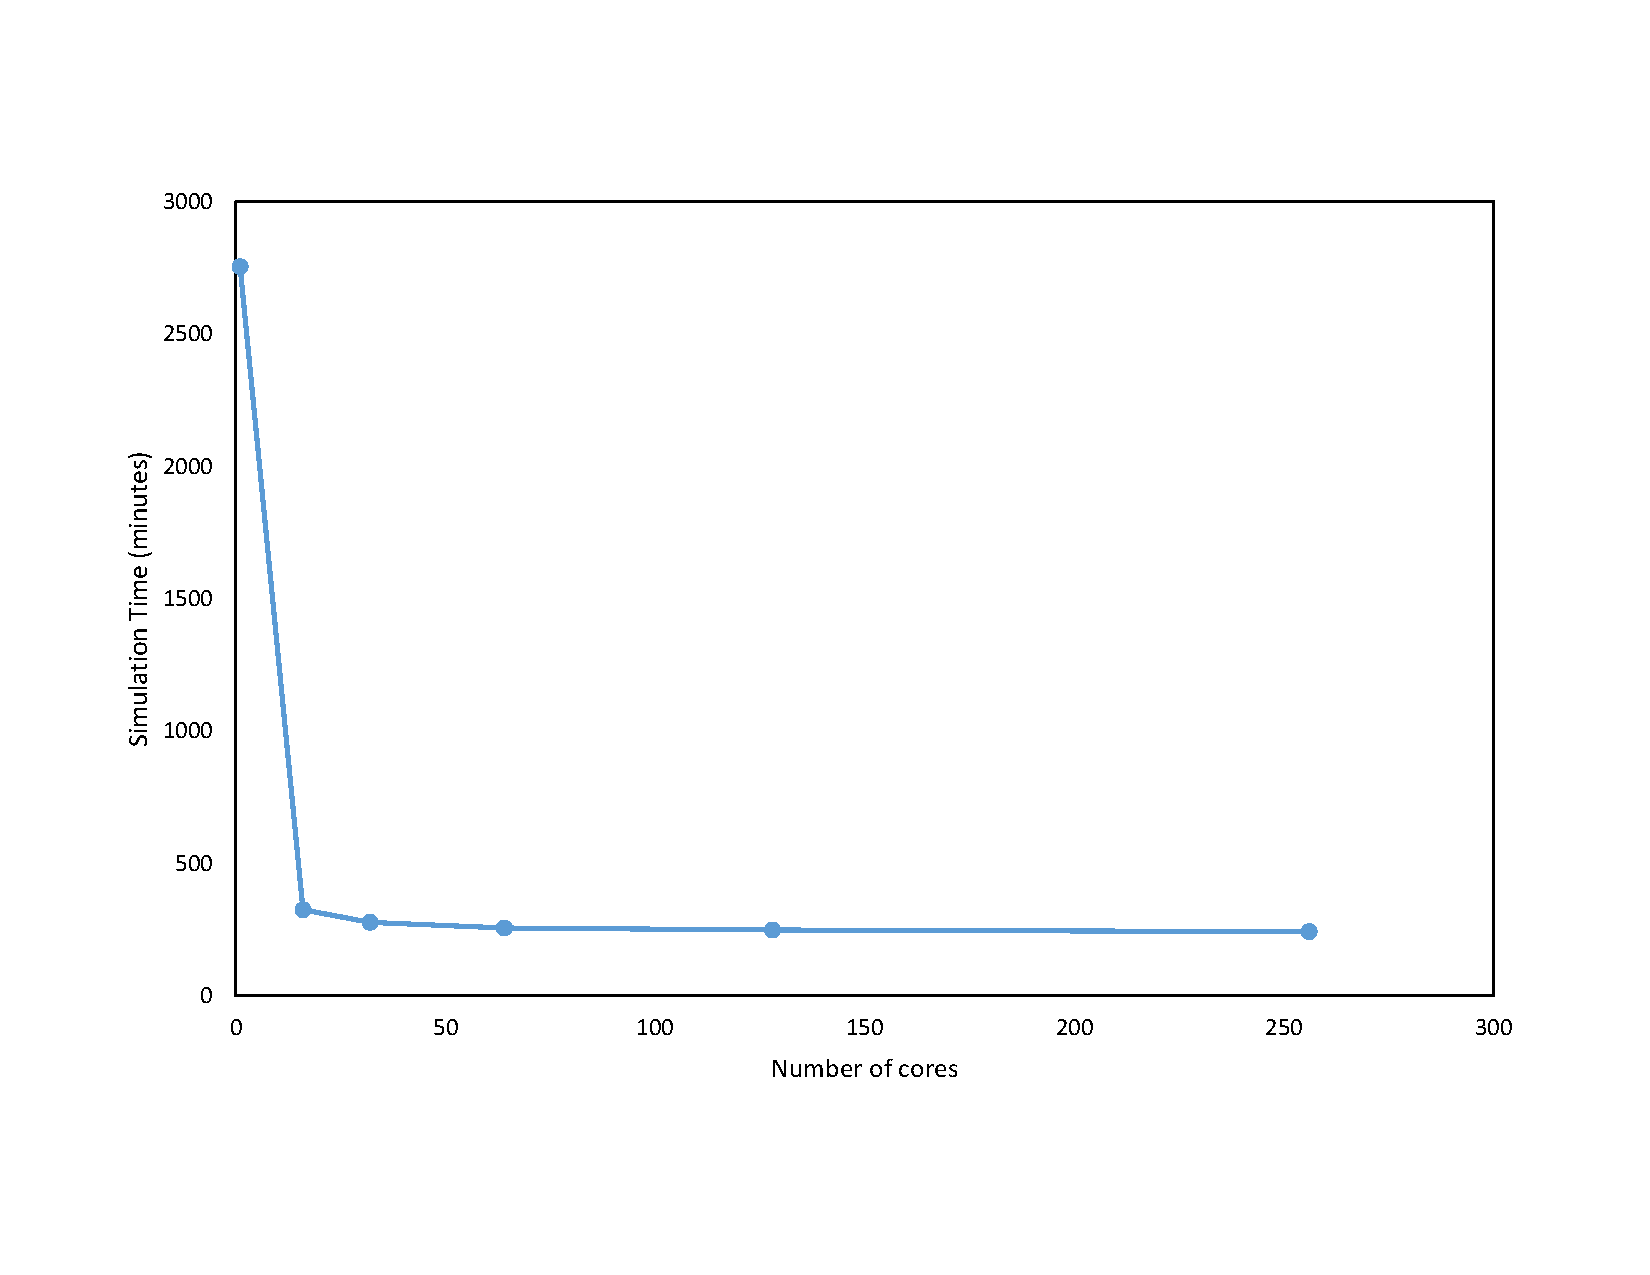
\includegraphics[scale=0.5]{rslts_DEM_2mm_timing.pdf}
\caption{The variation in the amount of time taken for the simulation as a function of \# of cores}
\label{fig:rslts_DEM_2mm_timing}
\end{figure}	

Pure timing studies are not really a good measure to represent the parallel performance of a program. 
Speedup of a parallel program indicates the speed increase of the program when it is run on more 
compute cores compared to the wall clock time when it is run in serial. It is the most common way to 
represent the parallel performance. Speedup is the ratio of the time taken to run the program in serial 
to the time taken by the program to run in parallel as shown in Equation \ref{eqn:rslts_DEM_Speed_Up}. 
For an ideally parallelized program, the speedup is 'n' times, where n is the number of cores used.\\

\begin{align}
\textit{Speedup} = \frac{\textit{Serial Wall Clock Time}}{\textit{Parallel Wall Clock Time}}
\label{eqn:rslts_DEM_Speed_Up}
\end{align}

Speedup does not take into account number of processors used in the simulation, thus another metric 
that is used to determine the s parallel performance is parallel efficiency. This metric is nothing by 
speedup divided by the number of cores used. Thus, parallel efficiency normalizes speedup and gives 
a fractional value of the ideal speedup a program achieves with the increase in the number of cores.\\

\begin{align}
\textit{Parallel Efficiency} = \frac{\textit{Serial Wall Clock Time}}{\textit{Parallel Wall Clock Time $\times$ $n_{cores}$}}
\label{eqn:rslts_DEM_parallel_efficiency}
\end{align}

    
 The figure \ref{fig:rslts_DEM_timing_studies} indicates that there is not a significant amount of 
speed improvement when 256 cores are used for the simulation over 128 cores. This speed decrease 
can be accounted to the communication time between the MPI processes. When the particles move 
from one section to another of the space, they are transfered as ghost particles from one process to 
another process. Thus, there is large amount of communication which is required. One of the issues of 
using a cluster with shared memory within the nodes but none in between nodes is that it has to rely 
on the networking infrastructure of the cluster which bottlenecks the communications thus leading to 
higher communication times. There are more sections present when 256 cores are used for the 
simulation, thus there is more communication in this system when compared to 128 core simulation. 
This excess communication makes the simulation slower though there is more processing power and 
it requires lesser time for other calculations. Another observation that can be made from the Figure 
\ref{fig:rslts_DEM_timing_studies} is that the particle size distribution simulation takes more time 
compared to the simulations with mono-sized particles of 1.59mm and 2mm, though the mean size of 
particles in the distribution is 2mm. The default profile provided by LIGGGHTS indicates that the time 
spent in calculating the particle-particle interaction forces was higher than the mono-sized 
simulations. The different diameters make the interaction forces more tedious thus, making it 
computationally more expensive. 

\begin{figure}[H]
\centering
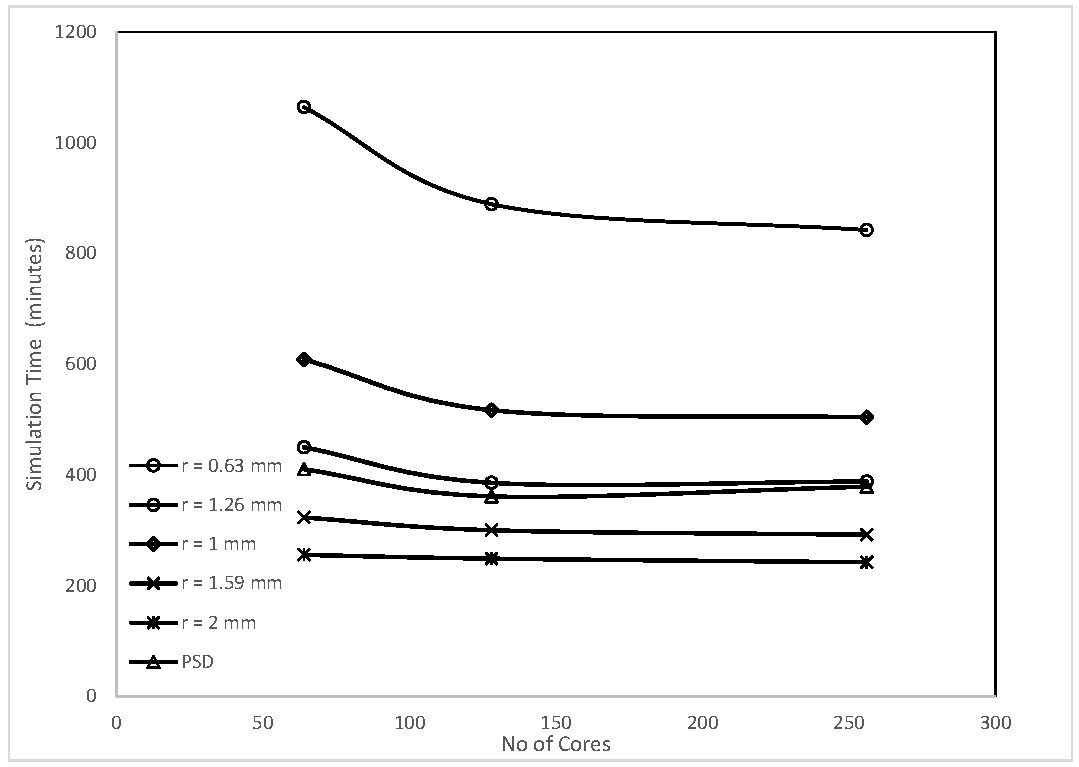
\includegraphics[scale=0.7]{rslts_DEM_timing_plots.pdf}
\caption{Time taken for a 10 second DEM simulation for diameters ranging from 0.63mm to 2mm and 
a particle size distribution ranging from 1mm - 3mm}
\label{fig:rslts_DEM_timing_studies}
\end{figure}
 The communication time in LIGGGHTS is indicated by the Modify time, which is the sum of the 
times required to transfer the rotating mesh from one process to the other. From the figure 
\ref{fig:rslts_DEM_percent_plot}, it can be seen the major chunk of the simulation time is taken up by 
the modify time. This is expected since the impeller is rotating at a very high speed of 2000 rpm. So, if 
the number of processes are increased the amount of time spent in transferring the mesh also 
increases. In the studies, the modify time as a percentage of the simulation increased from 82\% to 
about 90\%, when the core count was increased from the 64 cores to 256 cores. But, the using the 
higher number of cores reduces time taken to calculate particle-particle interaction as well as in 
neighbour calculation. Thus, a better implementation for meshing as well as decomposition of the 
geometry for faster simulations with higher core counts.

\begin{figure}[H]
\centering
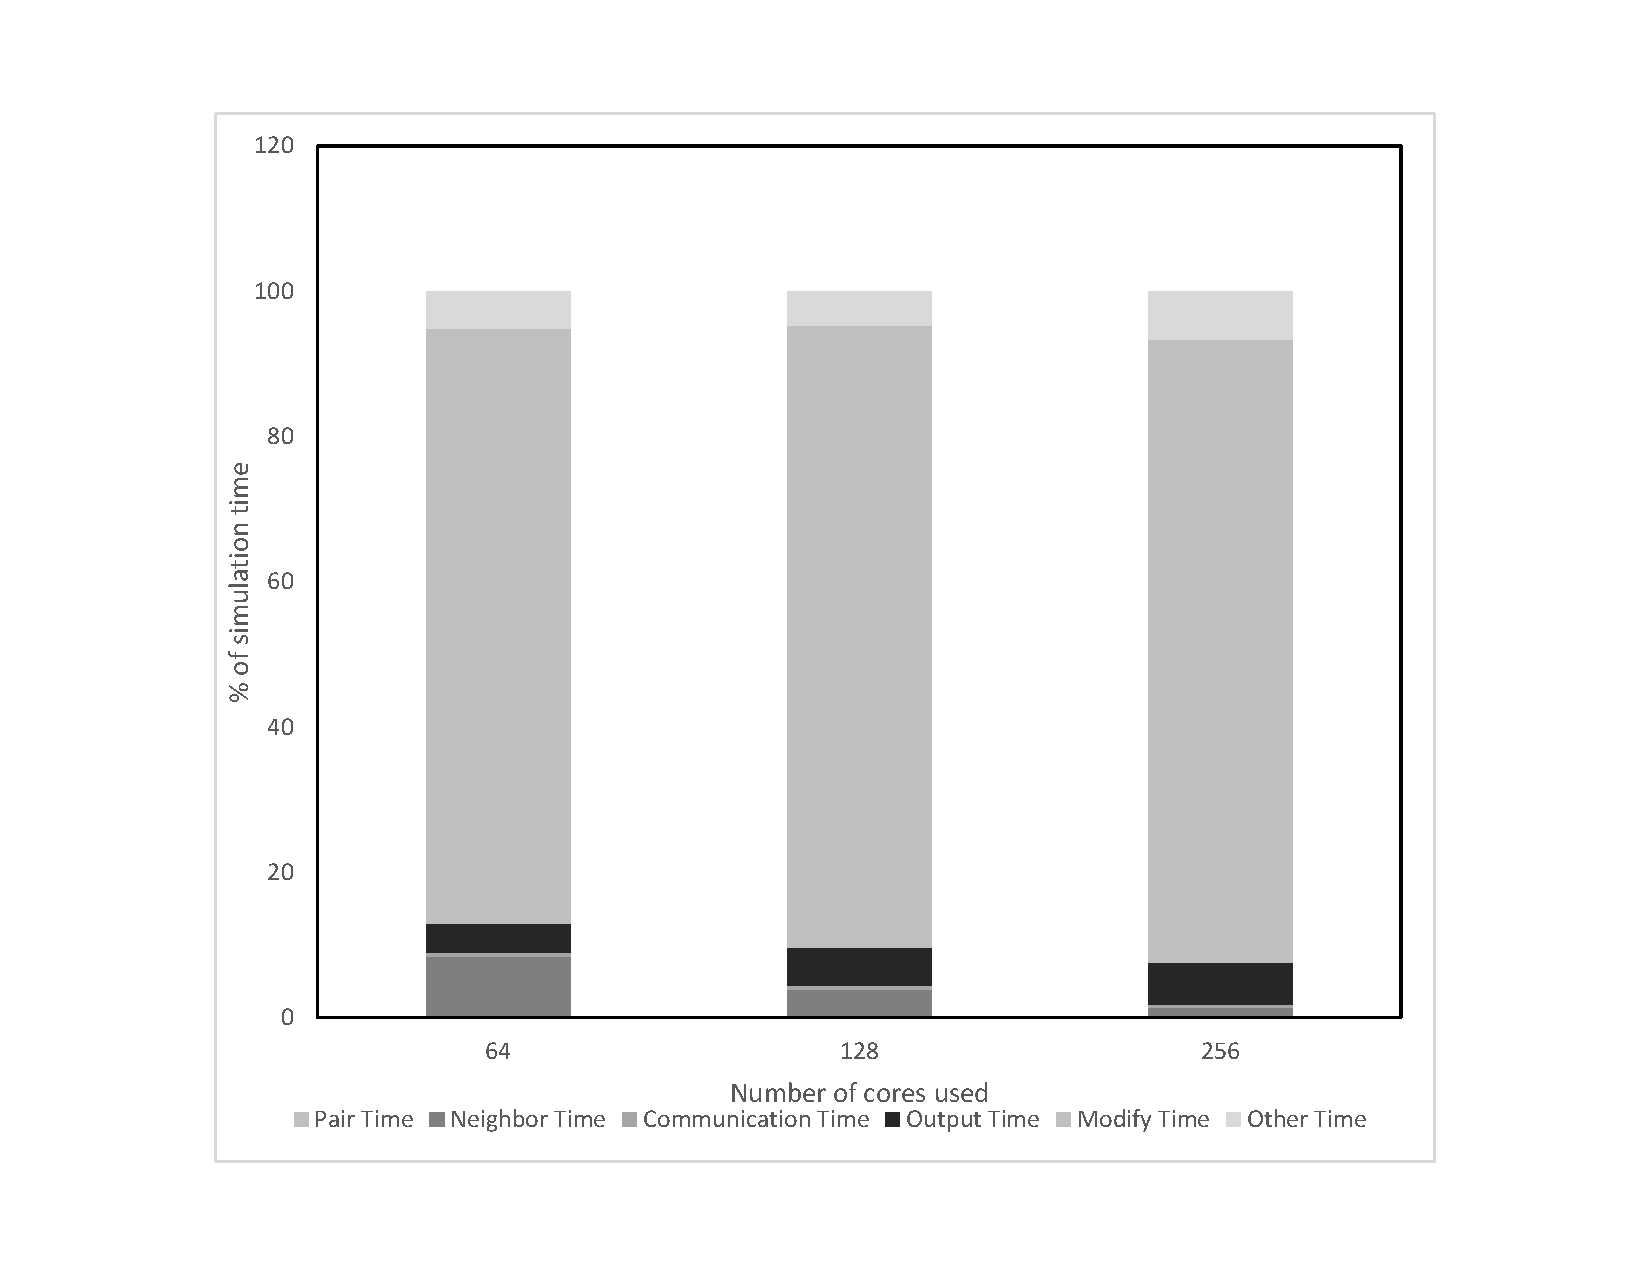
\includegraphics[scale=0.5]{rslts_DEM_percent_plot.pdf}
\caption{The variation in the amount of time taken for the simulation as a function of \# of cores}
\label{fig:rslts_DEM_percent_plot}
\end{figure}


\subsection{PBM}

%\subsection{PBM model validation without DEM data}
 
%\subsection{PBM model performance without DEM data}
% The PBM used for this study was initially tested without an DEM data using a constant value for the
%collisions. The PBM was tested on Stampede since it did not utilize the std libraries used to read
%and store the DEM data. This model was parallelised in the same manner as the mentioned above and 
%it achieved about 37\textit{x} speedup over the serial code. Table 
%\ref{table:rslts_performance_PBM_without_DEM} depicts the times of the experiments carried out 
%and performance improvments achieved.\\
%
%\begin{table}[ht]
%\caption{Performance studies of the PBM without the DEM data}
%\label{table:rslts_performance_DEM_without_DEM}
%\begin{center}
%\begin{tabulary}{\linewidth}{C|C|C|C|C|C}
%\hline
%\bf{Total cores in parallel}&\bf{MPI processes}&\bf{OMP threads}& \bf{Wall Time (seconds}& 
%\bf{SpeedUp}& \bf{Parallel efficiency}\\
%\hline
%$1$ & $1$ & $1$ & $222$ & $1.000$ & $1$\\
%$2$ & $1$ & $2$ & $147$ & $1.510$ & $0.755$\\
%$4$ & $1$ & $4$ & $109$ & $2.037$ & $0.509$\\
%$8$ & $1$ & $8$ & $103$ & $2.155$ & $0.269$\\		  
%$16$ & $2$ & $8$ & $41$ & $5.415$ & $0.338$\\
%$32$ & $4$ & $8$ & $21$ & $10.571$ & $0.330$\\
%$64$ & $8$ & $8$ & $10$ & $22.200$ & $0.347$\\
%$128$ & $16$ & $8$ & $6$ & $37.000$ & $0.289$\\
%\hline  		  
%\end{tabulary}
%\end{center}
%      
%\end{table}

\subsubsection{PBM model validation with DEM data}
 The population balance model implemented was considered to have an inlet flow of particles in the 
first compartment at a constant mass flow rate of 15 kilograms per hour. The particles were assumed 
to have a log normal distribution with minimum diameter of the particles being about 12 $\mu$m and the 
maximum of 2.1 mm with a mean of 0.453 mm and a standard deviation of about 0.62 mm. \\
The PBM used in this study employs an aggregation kernel that takes in account the formation of a 
larger particle from only two smaller particles. The ratio of the rate of formation and the rate of 
depletion due to aggregation helps us monitor whether the PBM satisfies the conservation of mass. 
Since this PBM takes into account the aggregation of only 2 particles at once, the ratio of the particles 
is expected to have a value of 0.5 during the aggregation process. Figure \ref{fig:rslts_PBM_ratio_plot_2mm}
 illustrates this ratio to be 0.5 throughout the simulation, validating the accuracy of the PBM used.\\
\begin{figure}[H]
\begin{center}
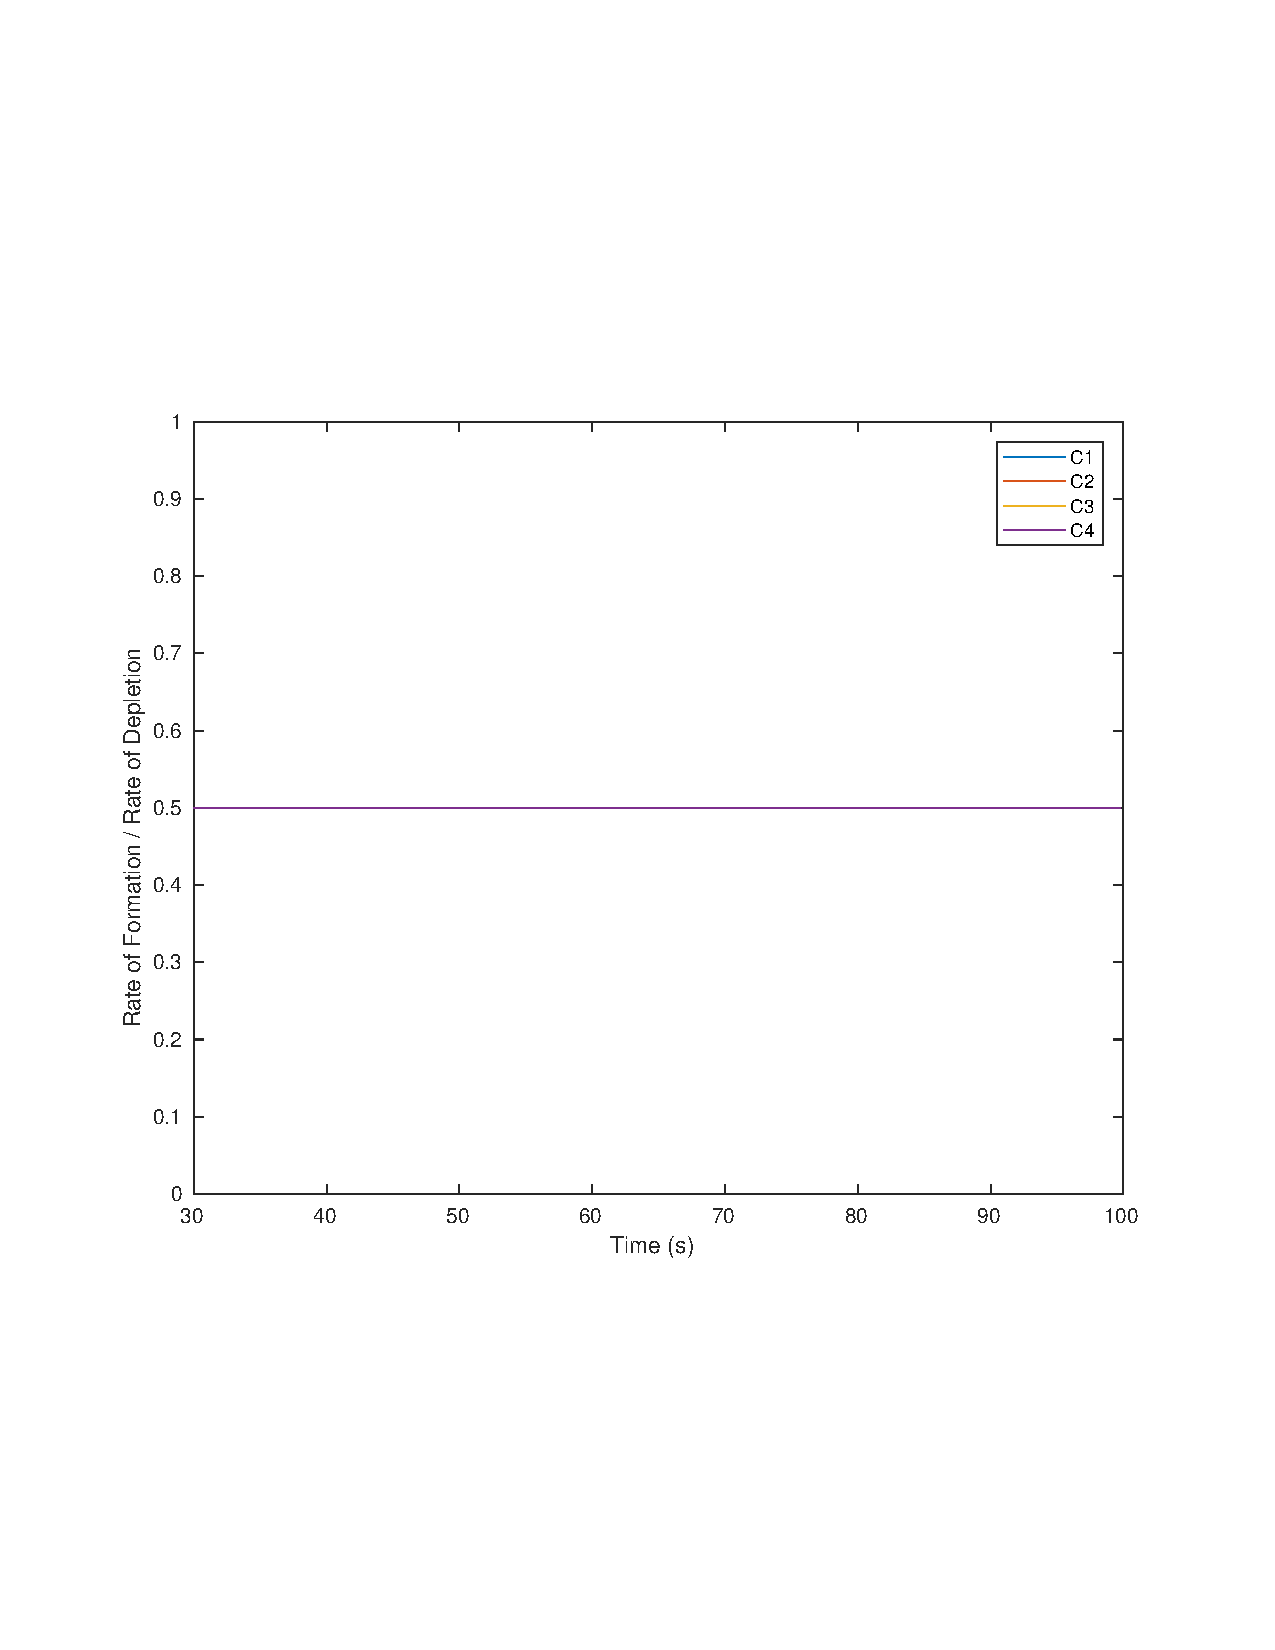
\includegraphics[scale=0.5]{rslts_PBM_2mm_validation.pdf}
\caption{The ratio of rate of formation to the rate of depletion of particles due to aggregation as a function 
of time.}
\label{fig:rslts_PBM_ratio_plot_2mm}
\end{center}
\end{figure}
Figure \ref{fig:rslts_PBM_d50_plots} shows four different particle size distribution plots at four 
different time instants. Figure \ref{fig:rslts_PBM_d50_plots}(\subref{fig:30s}) shows the distribution of 
the particles at 30 seconds, where we expect to have the highest number of the smaller particles. 
Since the degree of aggregation that has occurred is very low, thus there is a jump in the number of 
particles of the smaller size. The particle size distributions at 2 intermediate times of 50 seconds and 
75 seconds are plotted in Figures \ref{fig:rslts_PBM_d50_plots}(\subref{fig:50s}) and 
\ref{fig:rslts_PBM_d50_plots}(\subref{fig:75s}) respectively. These illustrate that there is an increase in 
the number of larger particles  and a subsequent decrease in the number of smaller particles. 
Figure \ref{fig:rslts_PBM_d50_plots}(\subref{fig:100s}) shows the distribution 
of the particle size at the end of the granulation process. It can be seen that the number of particles in 
the higher diameter bins increase.

\begin{figure}[H]
\begin{subfigure}{.5\textwidth}
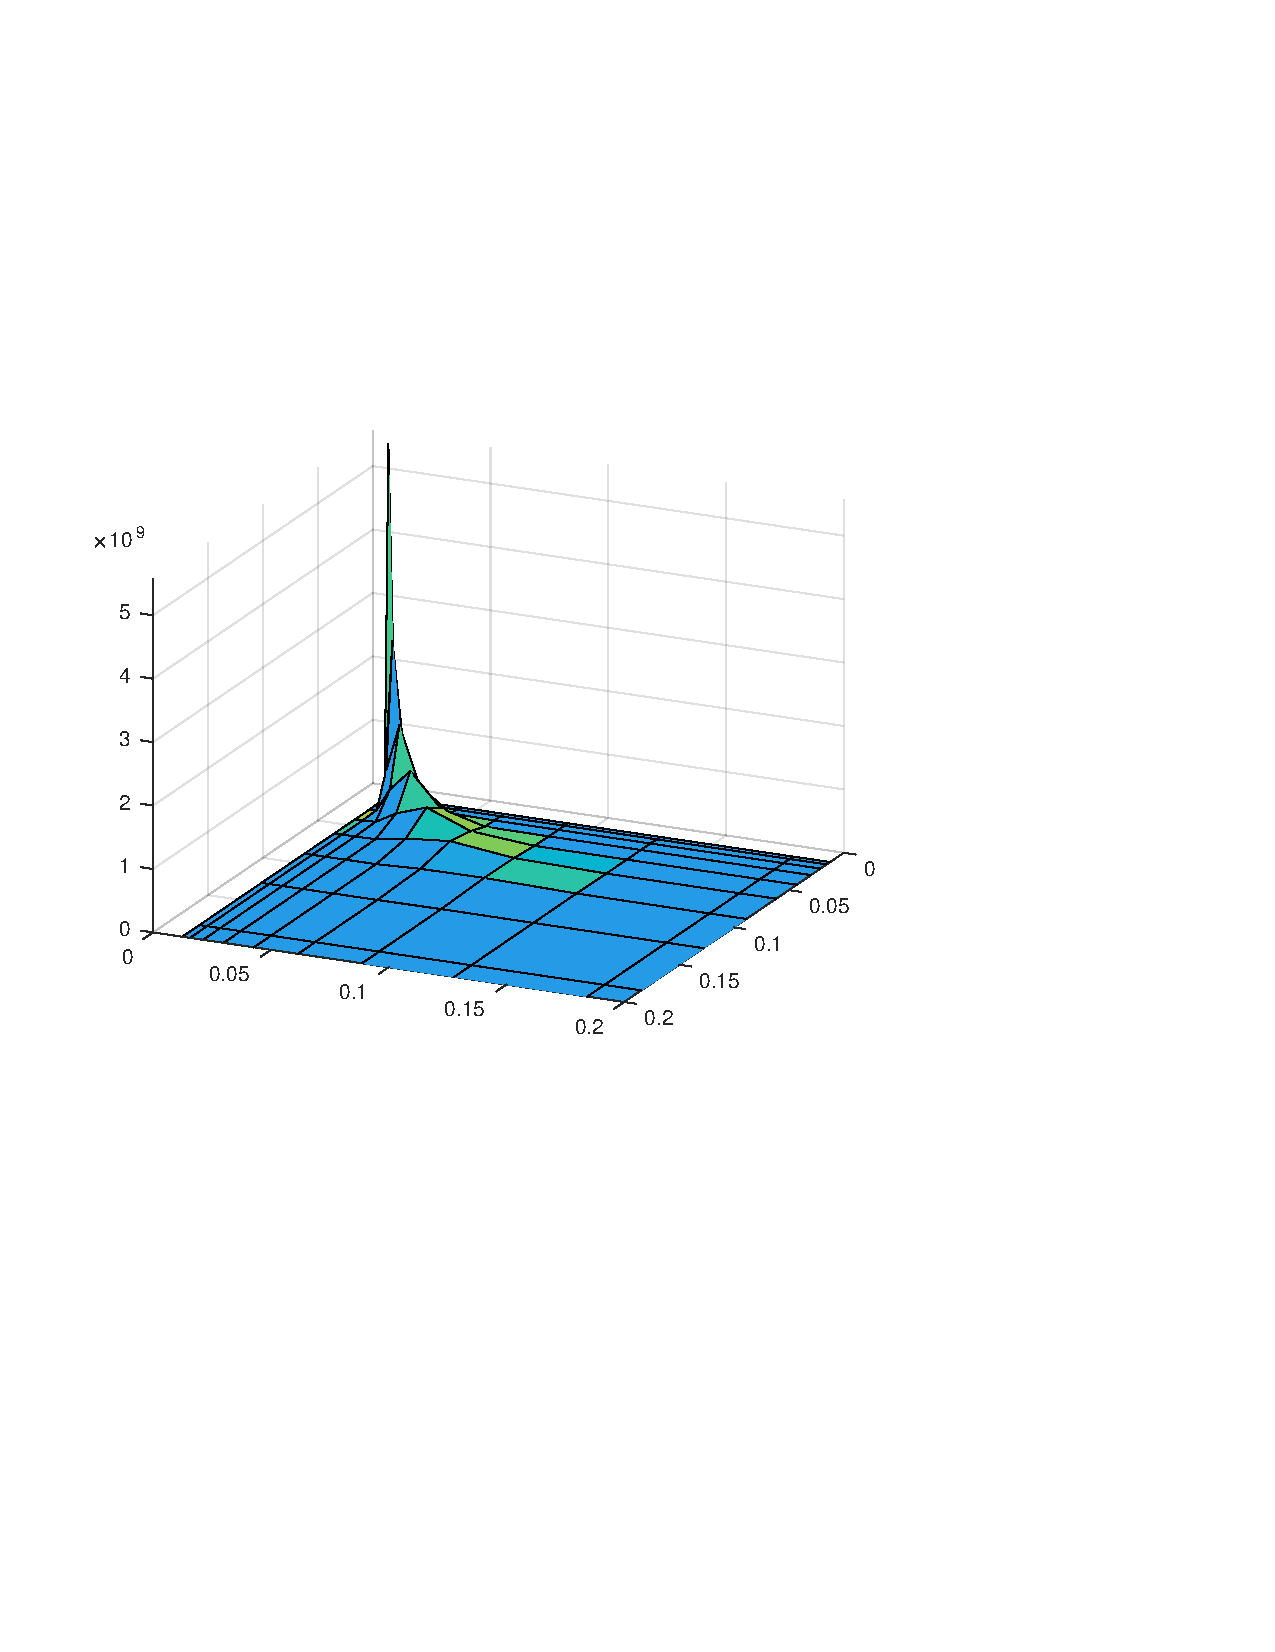
\includegraphics[scale=0.45]{rslts:PBM_30s_psd.pdf}
\caption{•}	
\label{fig:30s}
\end{subfigure}\hfill
\begin{subfigure}{.5\textwidth}

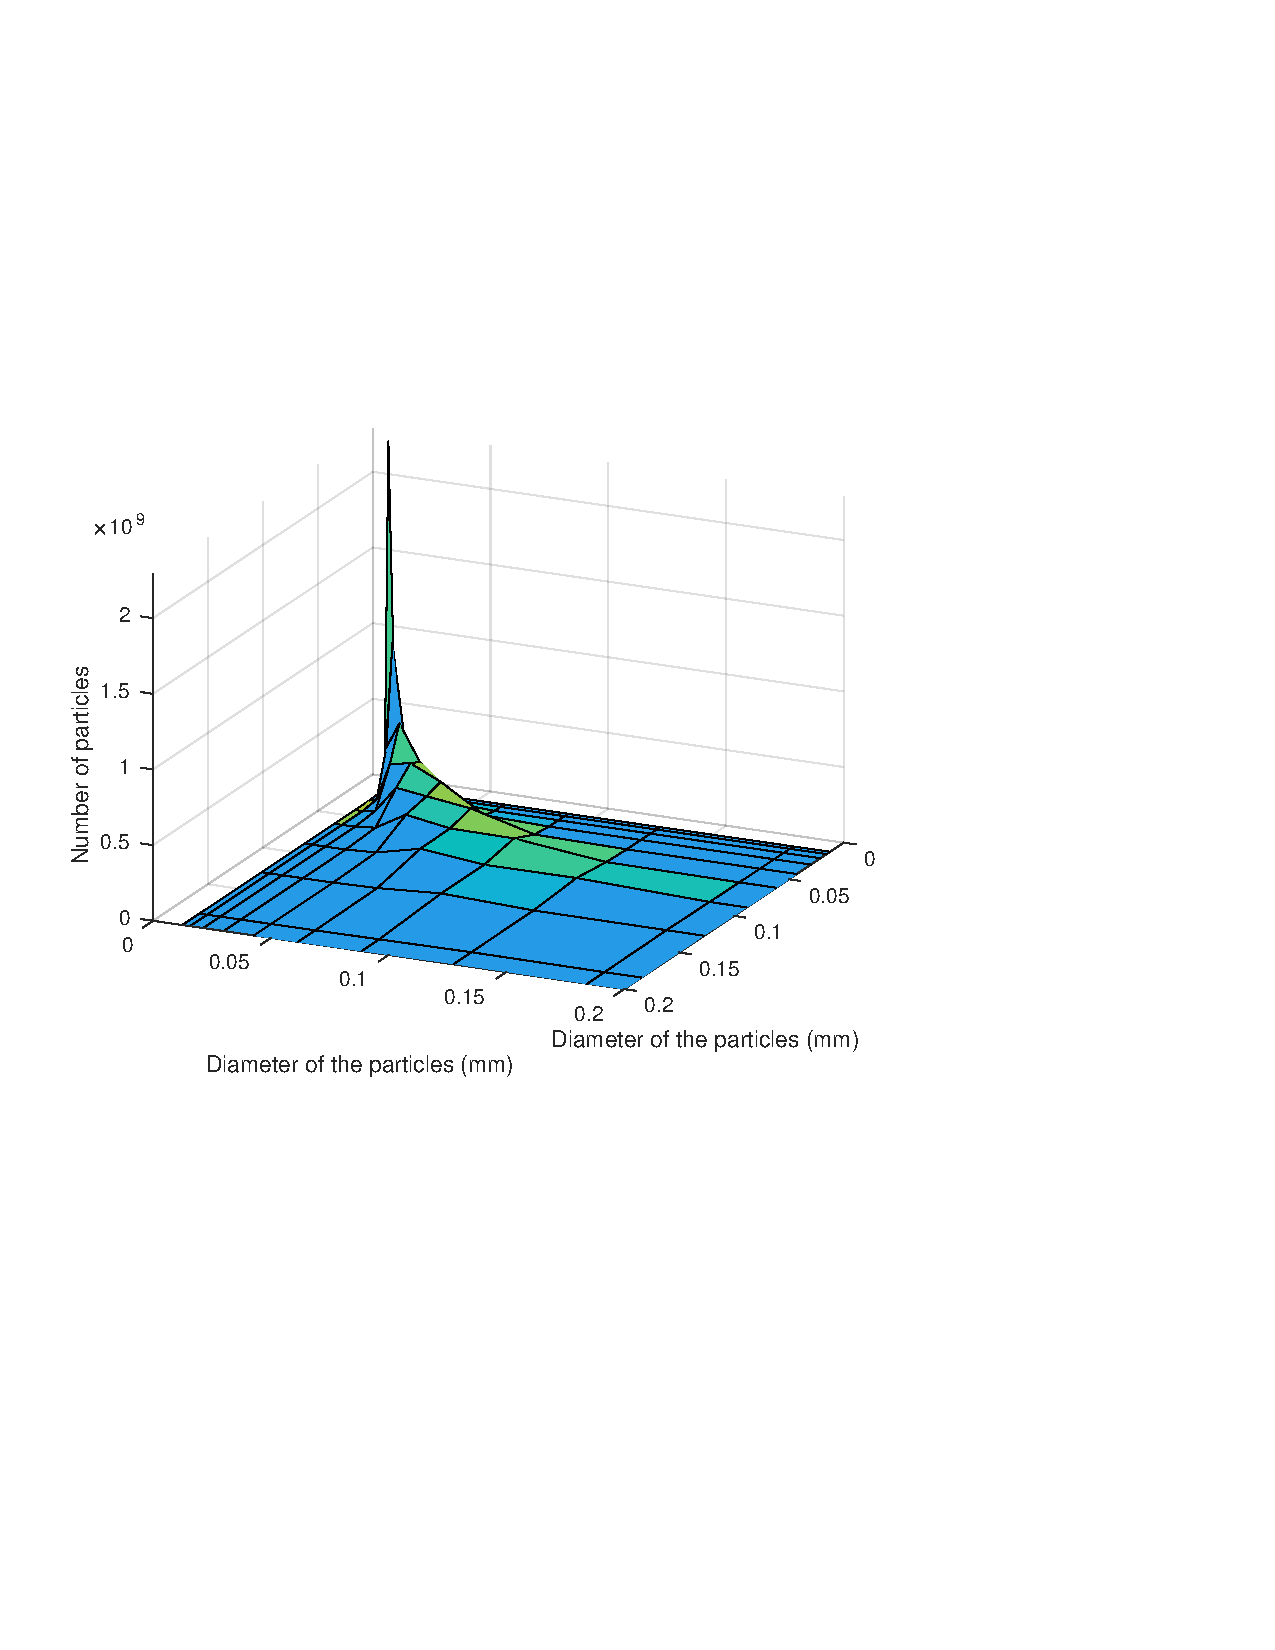
\includegraphics[scale=0.6]{rslts:PBM_50s_psd.pdf}
\caption{•}
\label{fig:50s}
\end{subfigure}
\begin{subfigure}{.5\textwidth}

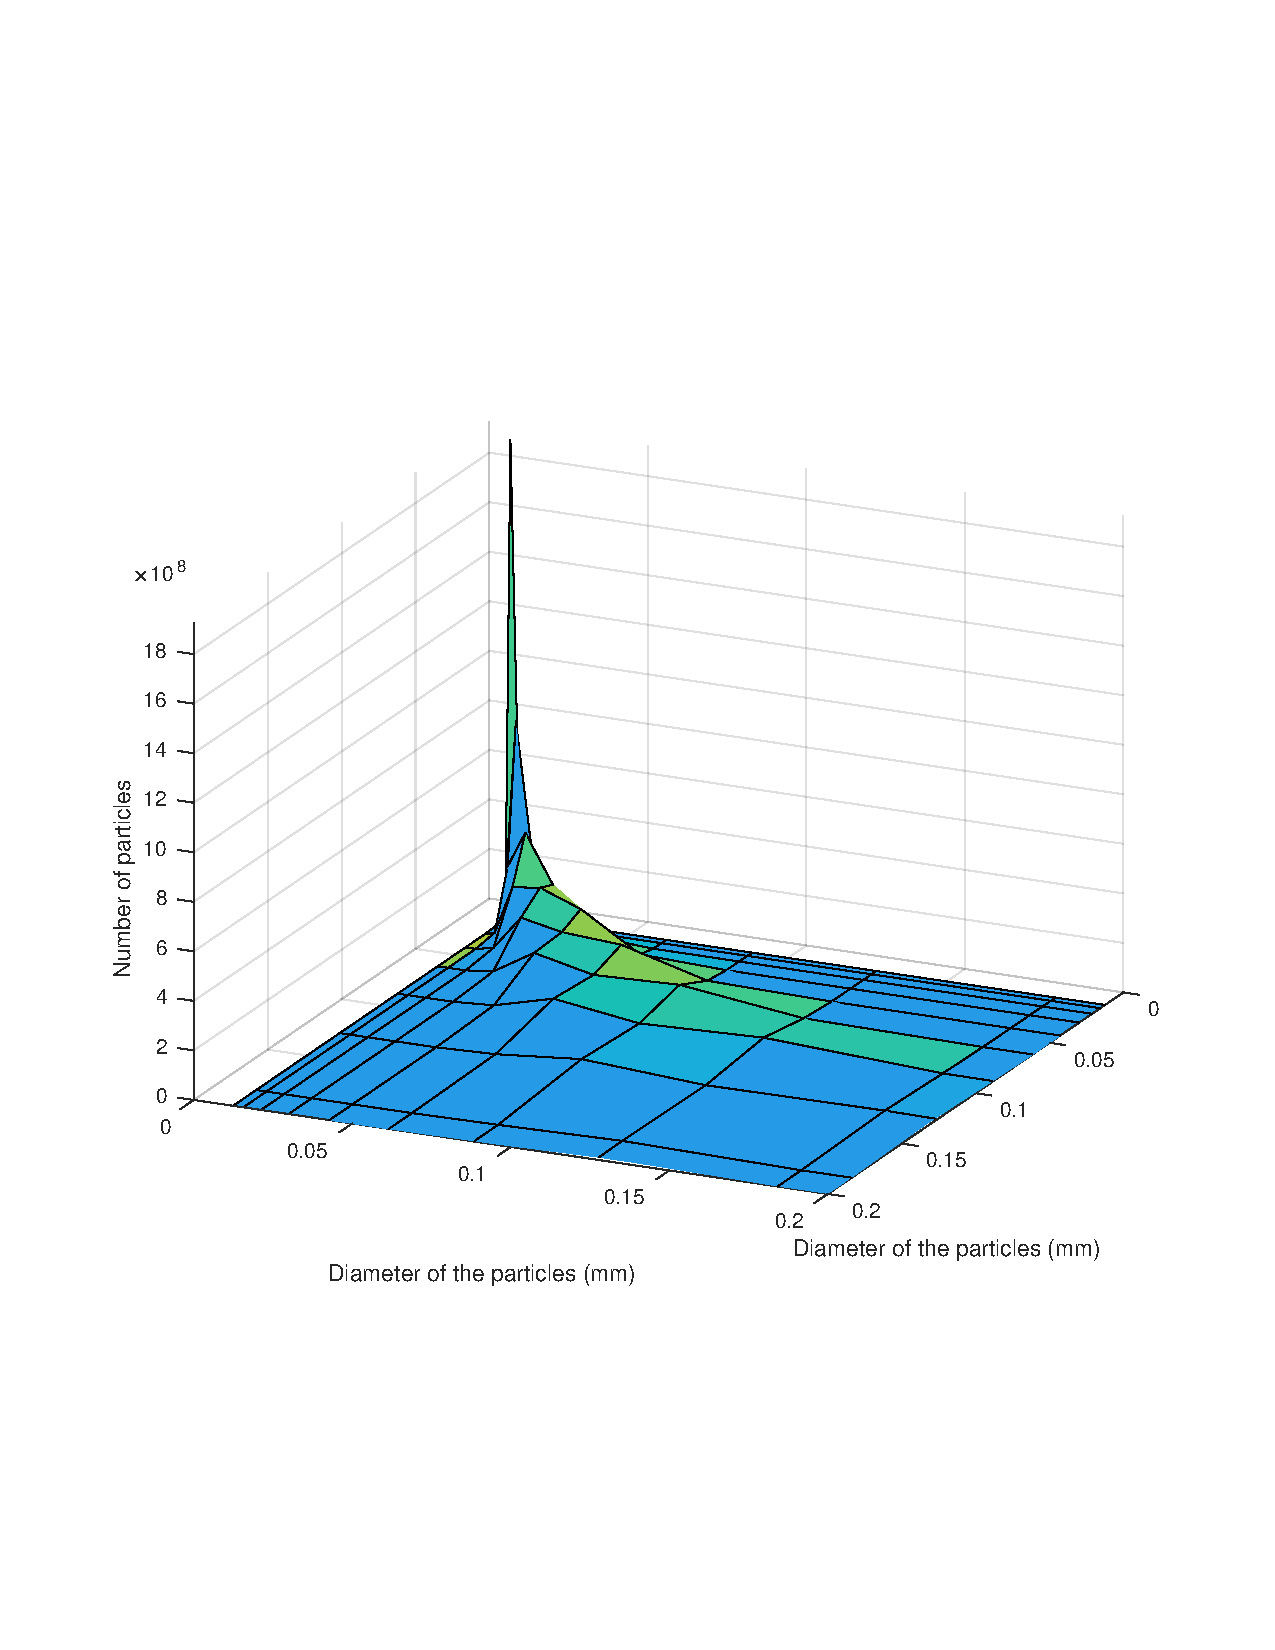
\includegraphics[scale=0.45]{rslts:PBM_75s_psd.pdf}
\caption{•}
\label{fig:75s}
\end{subfigure}\hfill
\begin{subfigure}{.5\textwidth}

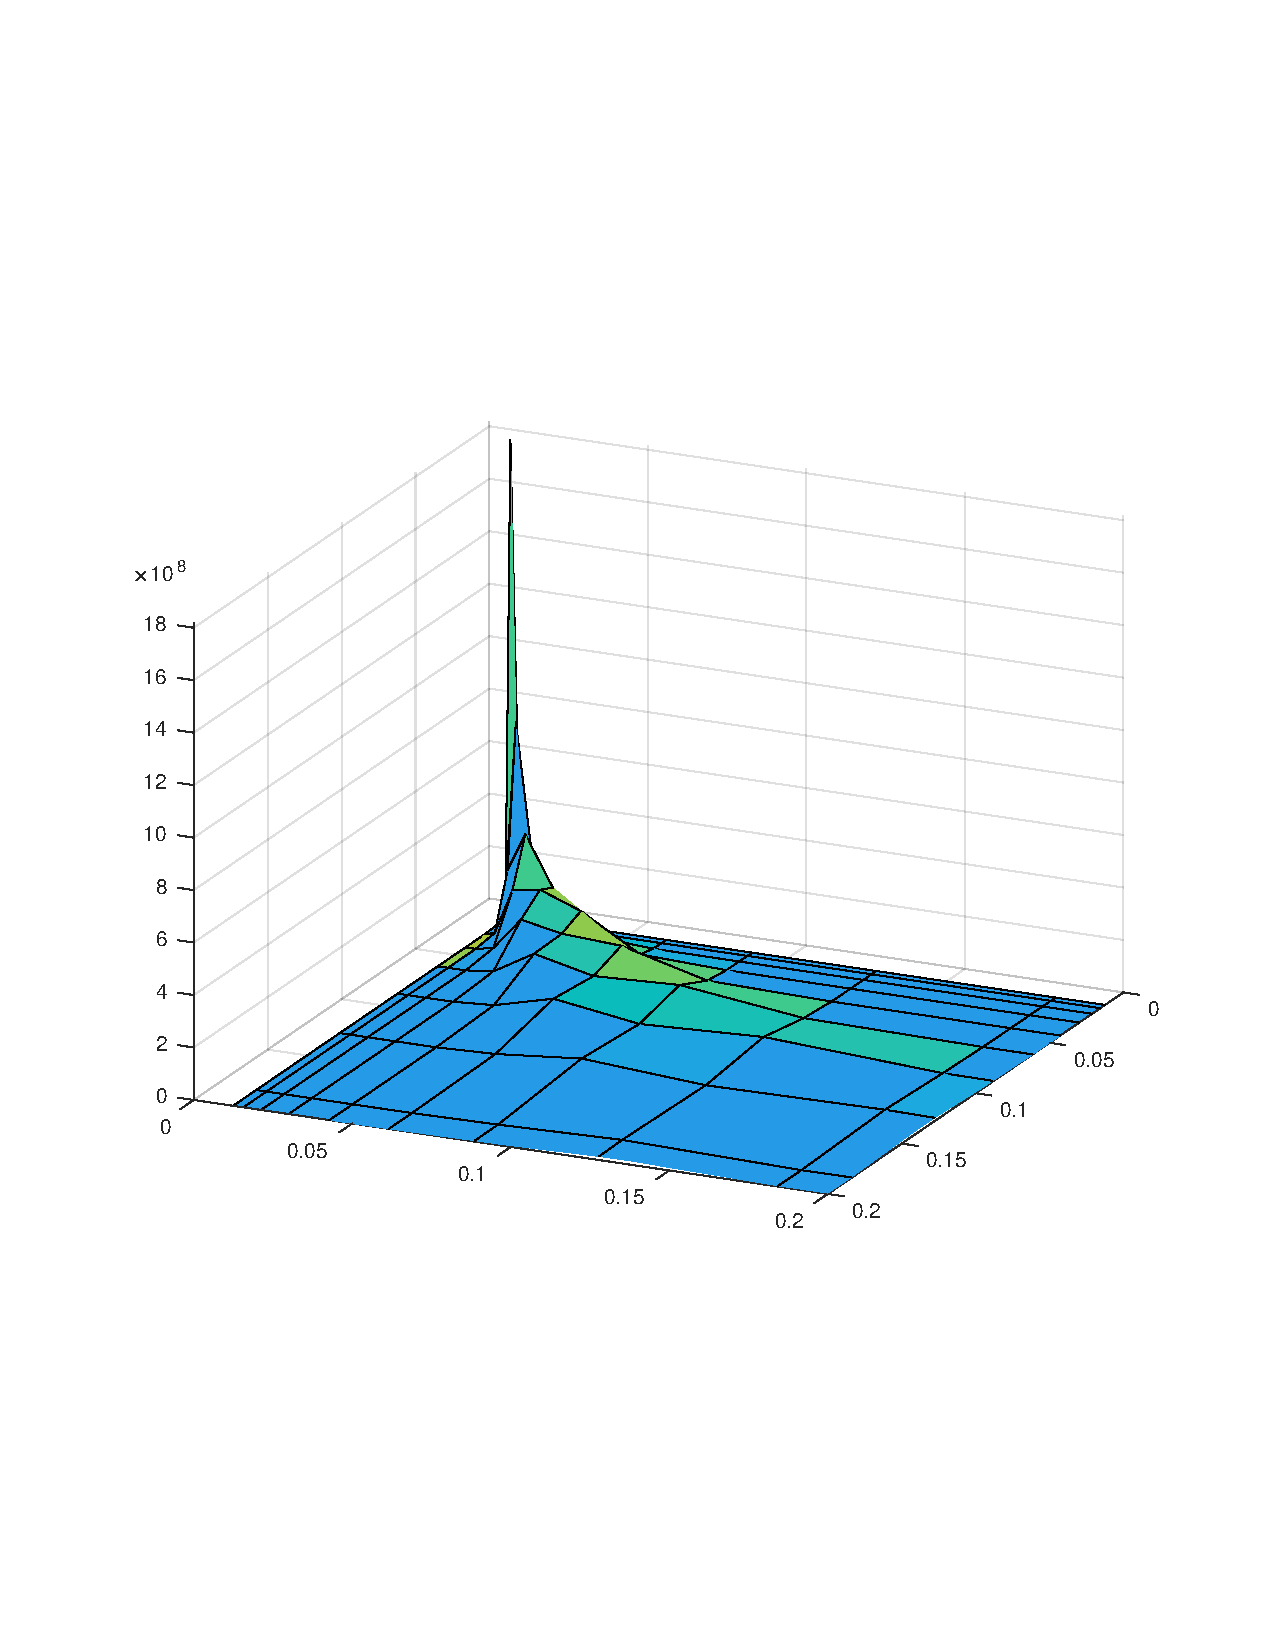
\includegraphics[scale=0.45]{rslts:PBM_100s_psd.pdf}
\caption{•}
\label{fig:100s}
\end{subfigure}
\caption{The number of particles inside all compartments with diameters less than 0.2 mm in 
mm after (\subref{fig:30s}) 30s (\subref{fig:50s}) 50s (\subref{fig:75s}) 75s and (\subref{fig:100s}) 
100s}
\label{fig:rslts_PBM_d50_plots}
\end{figure}   

\subsubsection{Parallel PBM performance studies}
 The PBM was run for the results obtained from each of the aforementioned DEM simulations. 
Since the PBM has been parallelized using hybrid techniques, a combination of MPI and OMP cores 
were used to perform the simulations. Figure \ref{fig:rslts_PBM_timing_studies} shows the average time 
taken by a PBM simulation for a total of 100 seconds of the granulation process, which includes 25 
seconds of the mixing time and 75 seconds of granulation time. The time taken for simulating all DEM 
scenarios by a single set of core configuration of in less than 10\% of each other, thus, an  average 
time for a single core configuration was used to illustrate the performance. Figure 
\ref{fig:rslts_PBM_timing_studies} shows that the program scales really well to about 32 cores but then, 
the improvement in the performance is negligible. The times represented have the core configurations 
of only MPI up till 16 cores after which 32, 64 and 128 core simulations employed 8 OMP threads 
each. The scaling with the only MPI cores shows great increase in performance. \\
\begin{figure}[H]
\centering
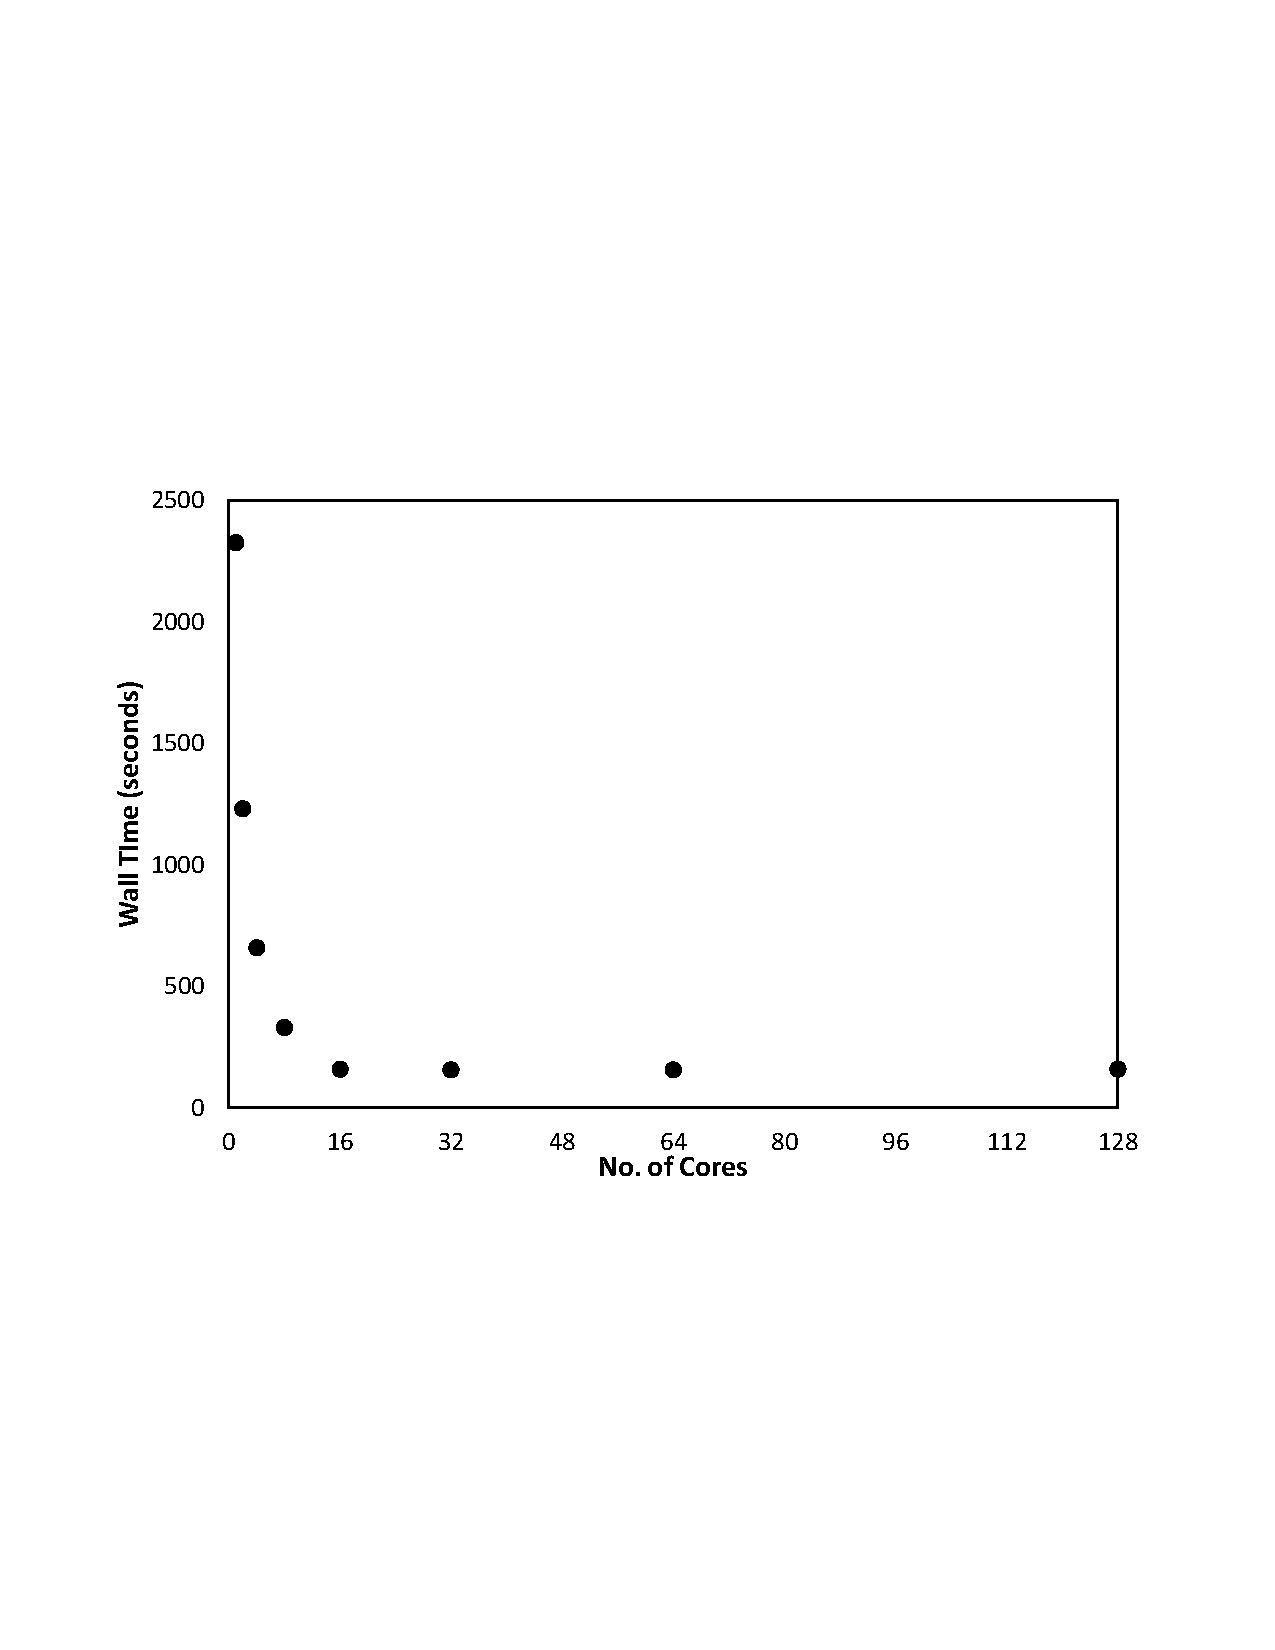
\includegraphics[scale=0.7]{rslts_PBM_Time_analysis.pdf}
\caption{Average time taken to run the PBM simulation which consisted of 25 seconds of mixing time 
and 75 seconds of granulation time at different core configurations}
\label{fig:rslts_PBM_timing_studies}
\end{figure}


Figure \ref{fig:rslts_PBM_speed_up} depicts the speed up achieved by the hybrid parallel PBM code. It 
can be seen when the MPI cores used are increased from 1 to 16 cores the speed upp achieved is 
almost linear. This speed can be accounted to the way MPI has been implemented inside the code. 
Each compartment of the granulator is  offloaded on one MPI process, thus making 16 MPI processes 
the ideal since, the granulator has been divided into 16 compartments. When the number of cores 
were lesser than 16 cores, more than 1 compartment is sent to a single MPI process, this leads to a 
decrease in performance. The implementation of OMP on top of the MPI parallelization helps increase 
the performance by the about 10\%. The calculations inside the OMP parallel section of the code 
consists of large number of nested loop which have been known to be difficult to parallelize 
\citep{He2016} using the native C++'s OMP libraries. The amount of communication time spent in 
between these threads is much higher than the speed increase achieved by using higher number of 
cores. One thread waits for another thread to complete processing the outer loops thus lower 
performance increase is achieved by using the OMP implementation. \\

\begin{figure}[H]
\centering
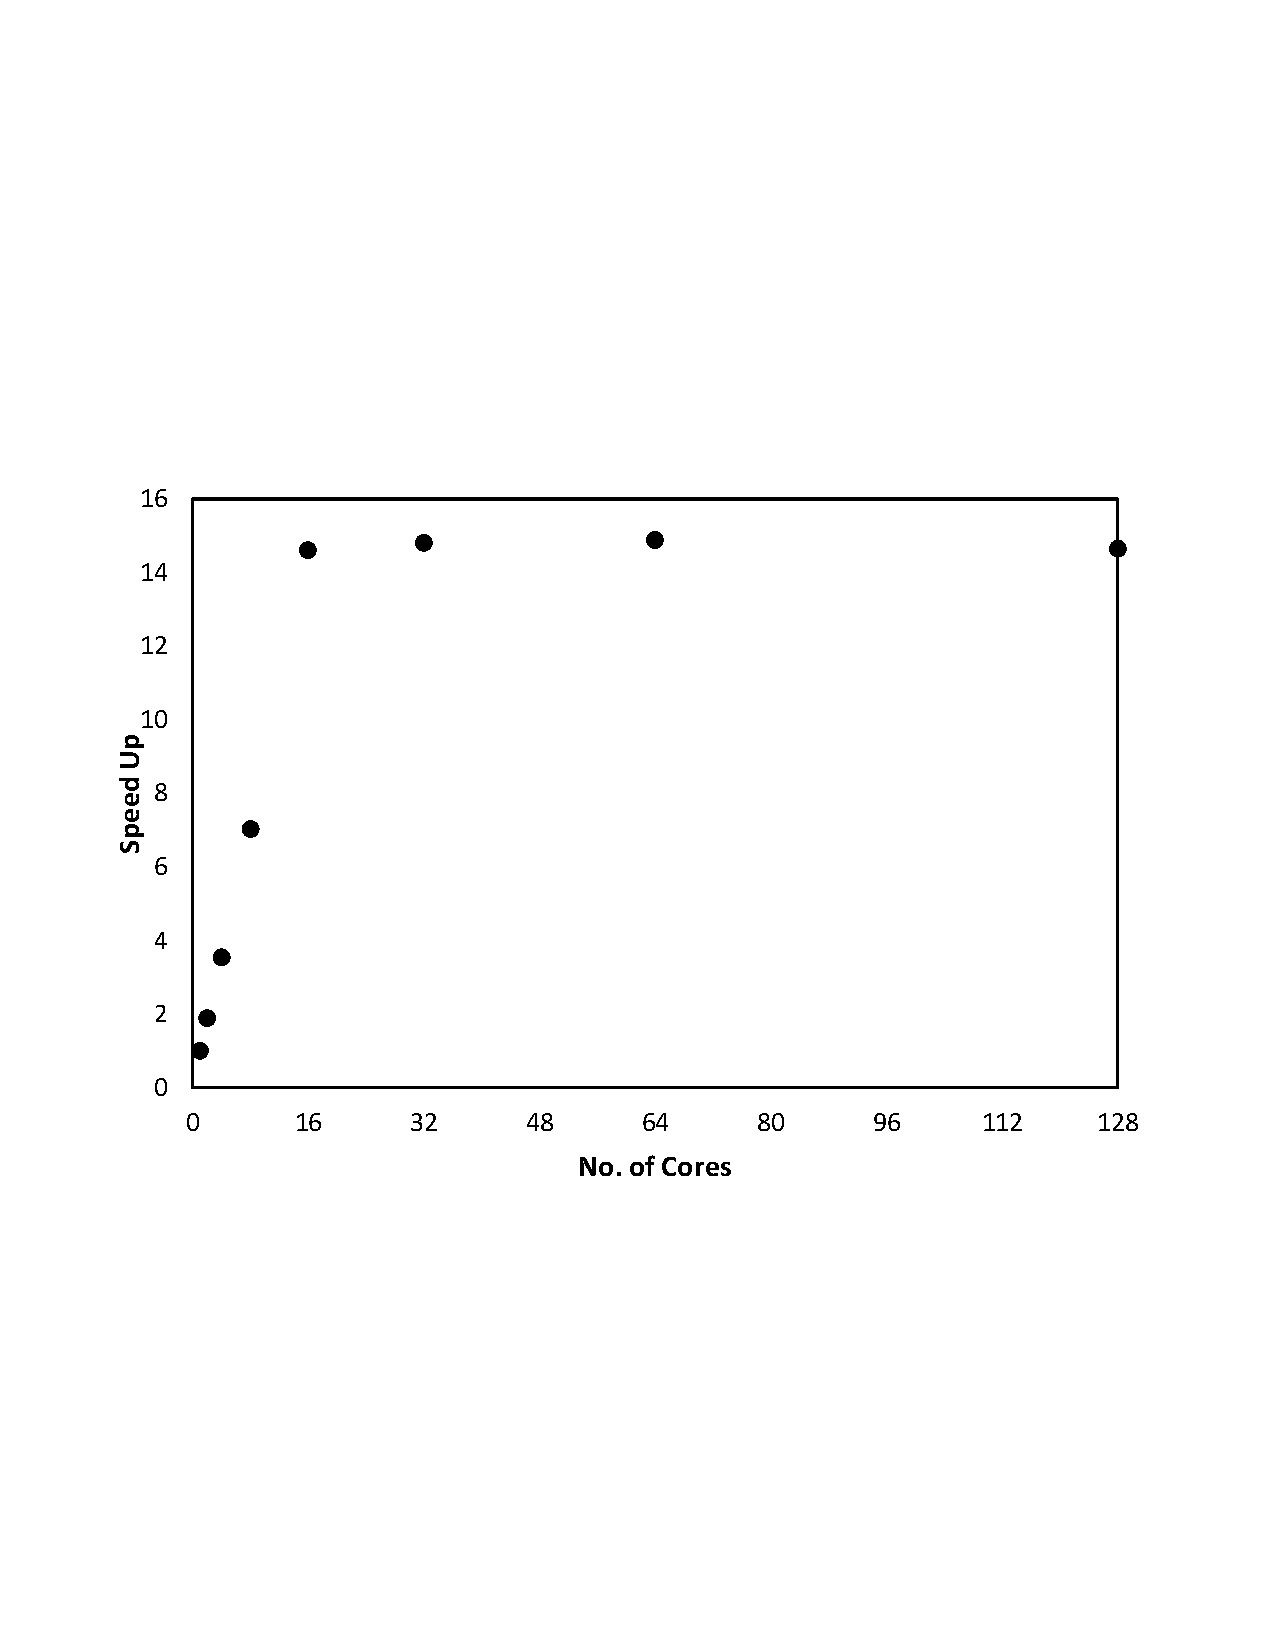
\includegraphics[scale=0.7]{rslts_PBM_Speed_Up.pdf}
\caption{The speedup achieved by the hybrid parallel implementation of the PBM program. It can be 
seen the inital speedup upto 16 cores as expected as from an ideal parallel program where as it 
becomes almost constant from 32 cores to 128 cores}
\label{fig:rslts_PBM_speed_up}
\end{figure}

A similar nature as above is observed in Figure \ref{fig:rslts_PBM_parallel_efficiency} where the parallel 
efficiency of the program has been plotted against the number of the cores used. This efficiency 
decreases as the number of cores used increase. The fall in efficiency initially up till 8 cores is steep as 
the communication time in between the MPI process decreases the efficiency, deviating its value from 
the ideal of 1 to about 0.4. But with the increase in the MPI processes to 16 and then the 
implementation of OMP the efficiency decreases as there is no major increase in the performance 
when compared to the increase in the number of cores used. The efficiency falls to as low as 11\% 
when 128 cores are used. Thus, there is scope for improving the OMP parallelizing the program 
especially where nested loops are present to decrease communication times.

\begin{figure}[H]
\centering
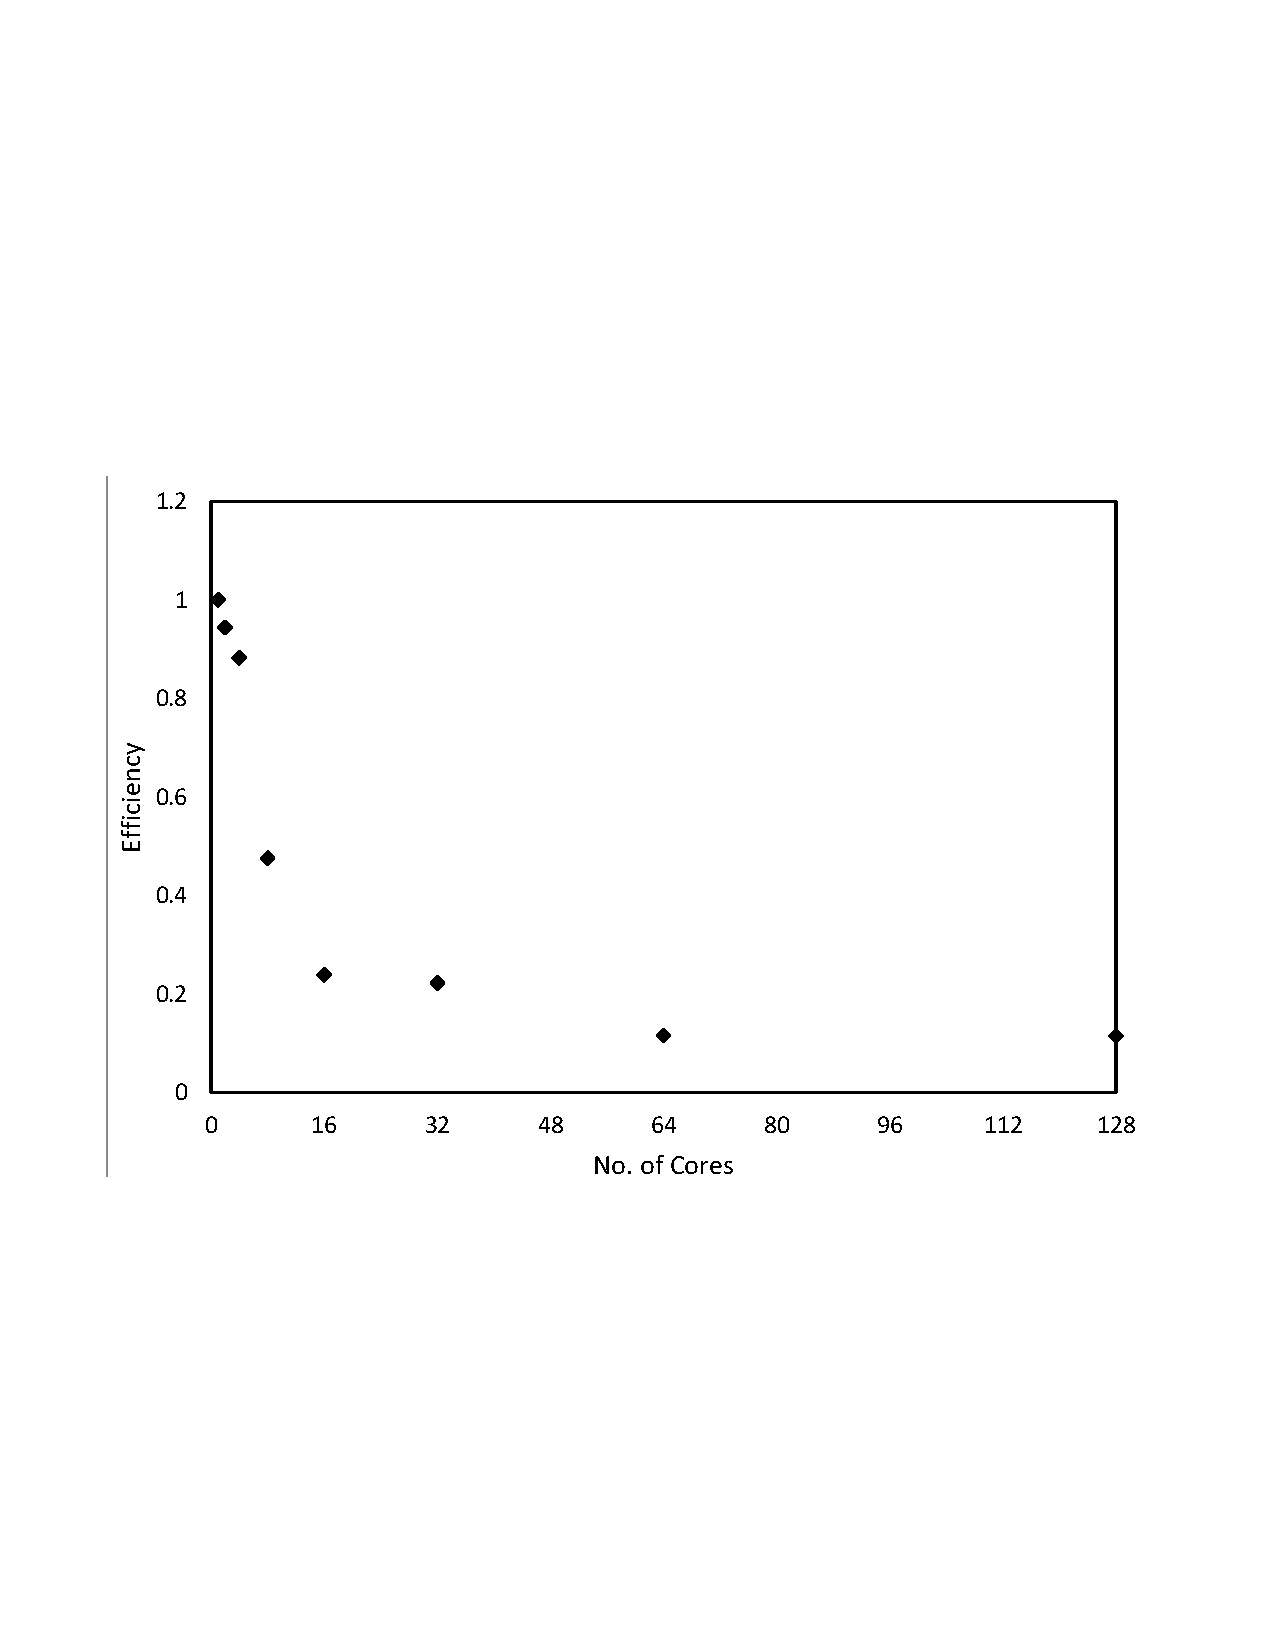
\includegraphics[scale=0.7]{rslts_PBM_Efficiency.pdf}
\caption{The parallel efficiency for the hybrid (MPI + OMP) parallelized PBM code. The efficiency of the 
code decreases as the number of cores are increased. The higher number of cores have very low 
efficiency of about 11\% which depicts that there is large time being spent in communication in 
between the cores.}
\label{fig:rslts_PBM_parallel_efficiency}
\end{figure}

\subsection{DEM + PBM physics}
 Micro-scale simulations provide an insight about the physics of the system usually by tracking 
each particle. This micro-scale simulation data is useful for the development of macro-scale 
mechanistic models which take into account the dynamics of bulk of the particles and not individual 
particles. A similar approach has been implemented in this work, where a mechanistic aggregation 
kernel was developed from the DEM particle-particle collisions. Thus, the aim of this section is to 
illustrate that the physics of the system does not change to a great extent with the change in the size 
of the particles or the distribution of the particles.\\
Two simulations from the current scenario will be compared, the DEM + PBM simulation of the 2mm 
mono-sized particle and the second being the simulation where the inserted particles were in a size 
distribution. Figure \ref{fig:rslts_PBM_psd_ratio} shows the ratio of rate of formation to the rate of 
depletion, both due to aggregation. The ratio obtained is 0.5 which indicates that the PBM is stable. 
Figure \ref{fig:rslts_PBM_psd_ratio} is also similar to Figure \ref{fig:rslts_PBM_ratio_plot_2mm}, thus 
indicating they have similar stability throughout the granulation process. \\
One of the metrics to determine the physics of the system after a PBM simulation is to check the 
d\textsubscript{50} plots of the system after the granulation process. D\textsubscript{50} indicates the 
maximum diameter of particles that constitute 50\% of the total mass. These diameters vary along the 
length of the granulator since the granulated particles take time to pass through the granulator and 
that there is not enough liquid content in the later sections of the granulator to encourage the 
formation of granules. Thus, the d\textsubscript{50} for compartments in the latter section of the 
granulator is low. Figures \ref{fig:rslts_PBM_2mm_d50} and \ref{fig:rslts_PBM_psd_d50} show the 
d\textsubscript{50} plots of the mono-sized and psd respectively. It can be seen that both these plots 
have a similar behaviour when it comes to the nature of the increase of the d\textsubscript{50} during 
the granulation process. There is a difference of about 20\% difference in the final diameter of the 
particles predicted, which at the of micrometers does not affect the final product quality. This slight 
deviation is observed due to the sudden jump in the rate of the aggregation which increases when 
particles from one compartment with higher d\textsubscript{50} get transfered to the next 
compartment with a lower d\textsubscript{50}. But, the advantage of running the mono-sized 
simulation compared to the psd simulation is the time taken to simulate the DEM. It can be seen from 
Figure \ref{fig:rslts_DEM_timing_studies} that the 2mm mono-sized particle took about 1.6 times less 
than the psd simulation time for the DEM. Since the physics of both the systems are not different, 
using the mono-sized simulations for the DEM help save time on the overall simulations. 

\begin{figure}[H]
\centering
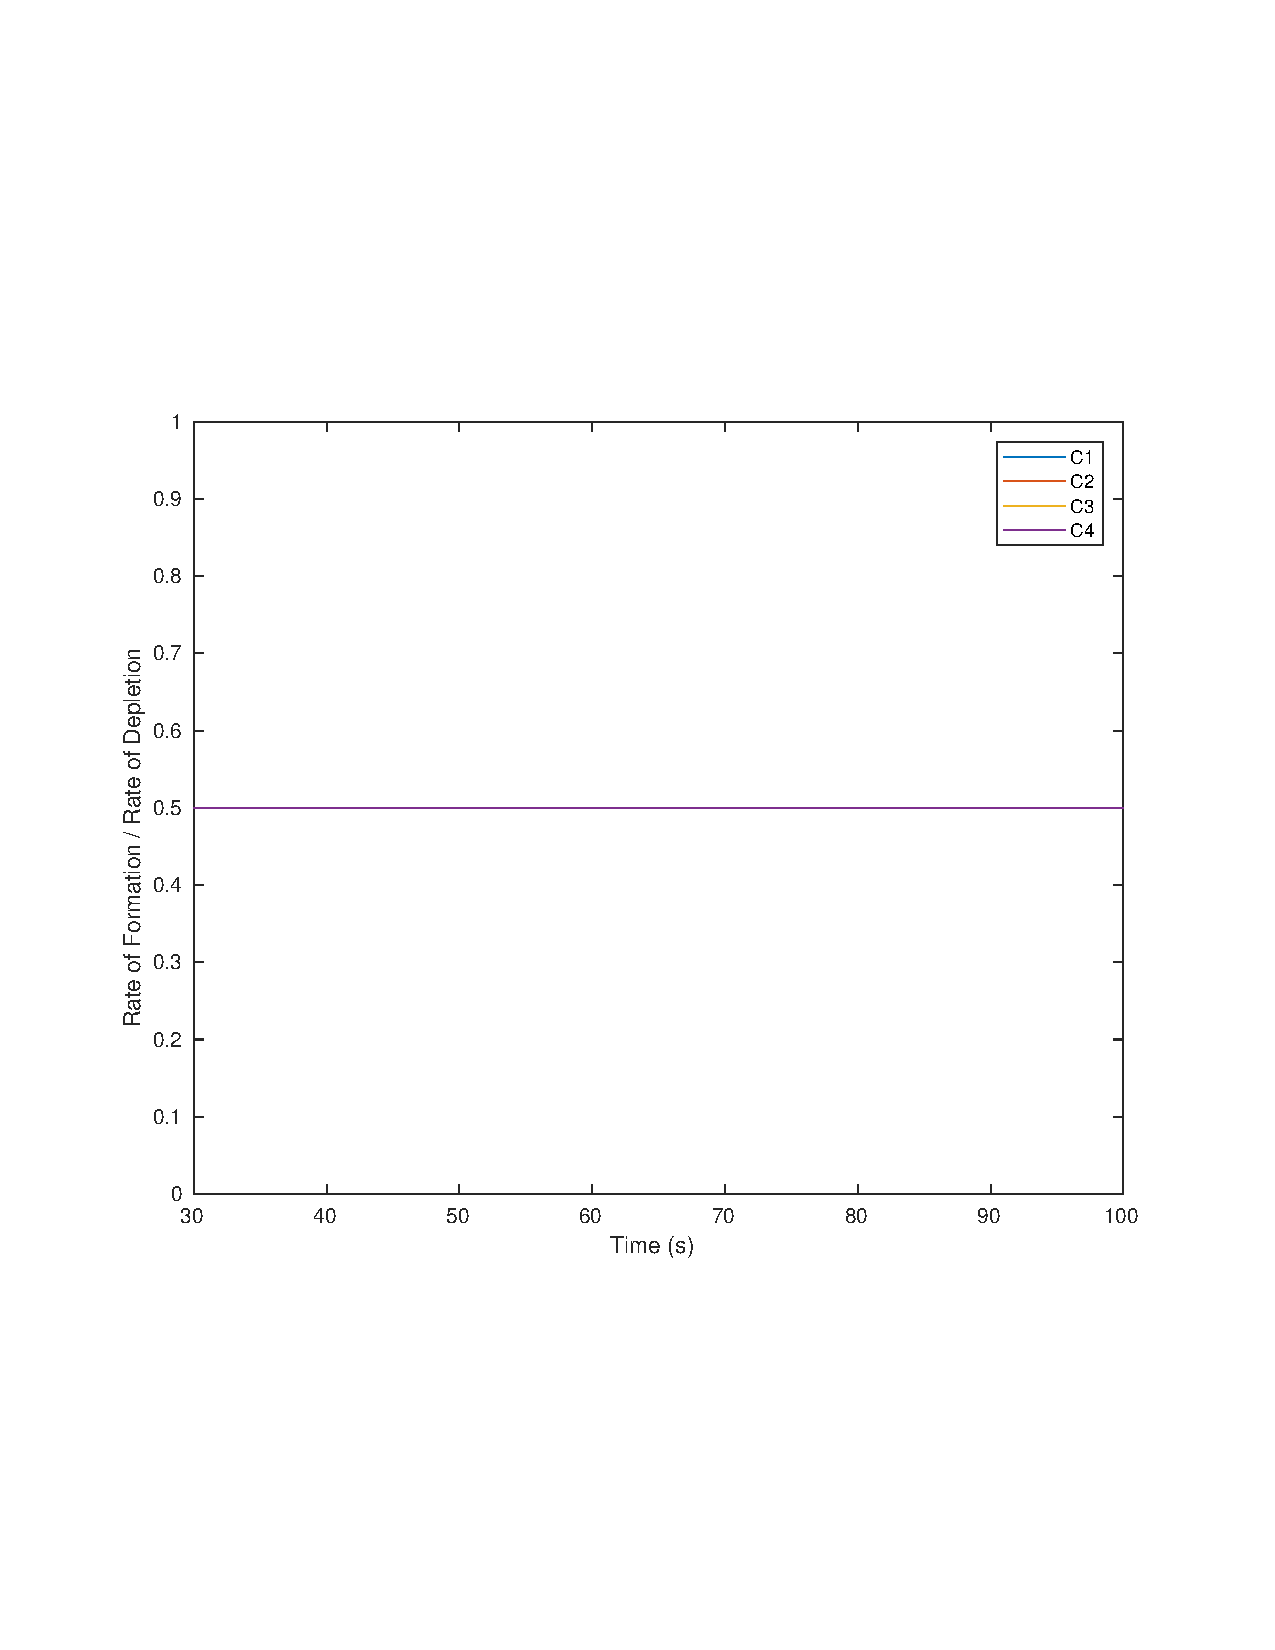
\includegraphics[scale=0.5]{rslts_pbm_psd_validation.pdf}
\caption{The ratio of rate of formation to the rate of depletion due to aggregation as a function of time. 
The constant value of 0.5 shows that the PBM is stable through the simulation time. This is similar to 
Figure \ref{fig:rslts_PBM_ratio_plot_2mm} which was for the 2mm mono-sized DEM simulation}
\label{fig:rslts_PBM_psd_ratio}
\end{figure}

\begin{figure}[H]
\centering
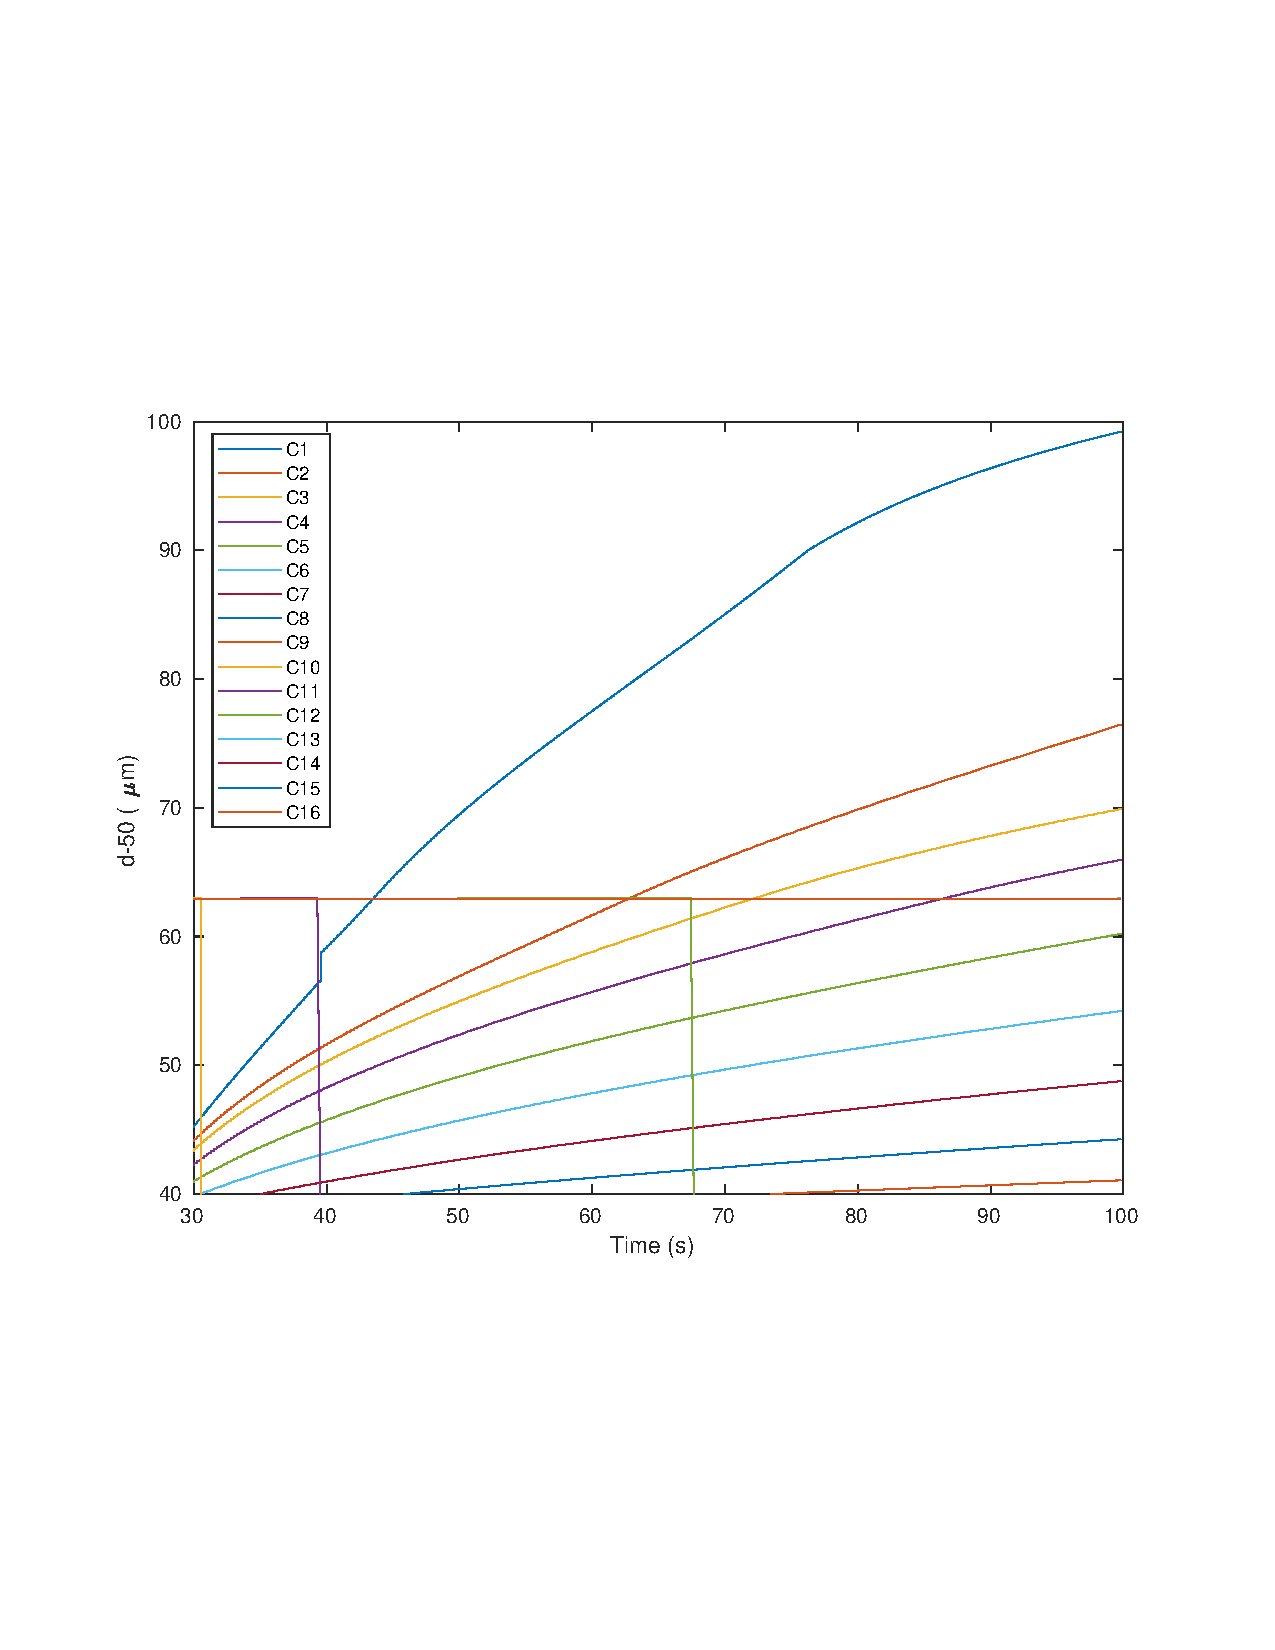
\includegraphics[scale=0.5]{rslts_pbm_d50_128_200.pdf}
\caption{d\textsubscript{50} plot after running the PBM for 100s for the 2mm mono-sized particle DEM 
simulation}
\label{fig:rslts_PBM_2mm_d50}
\end{figure}

\begin{figure}[H]
\centering
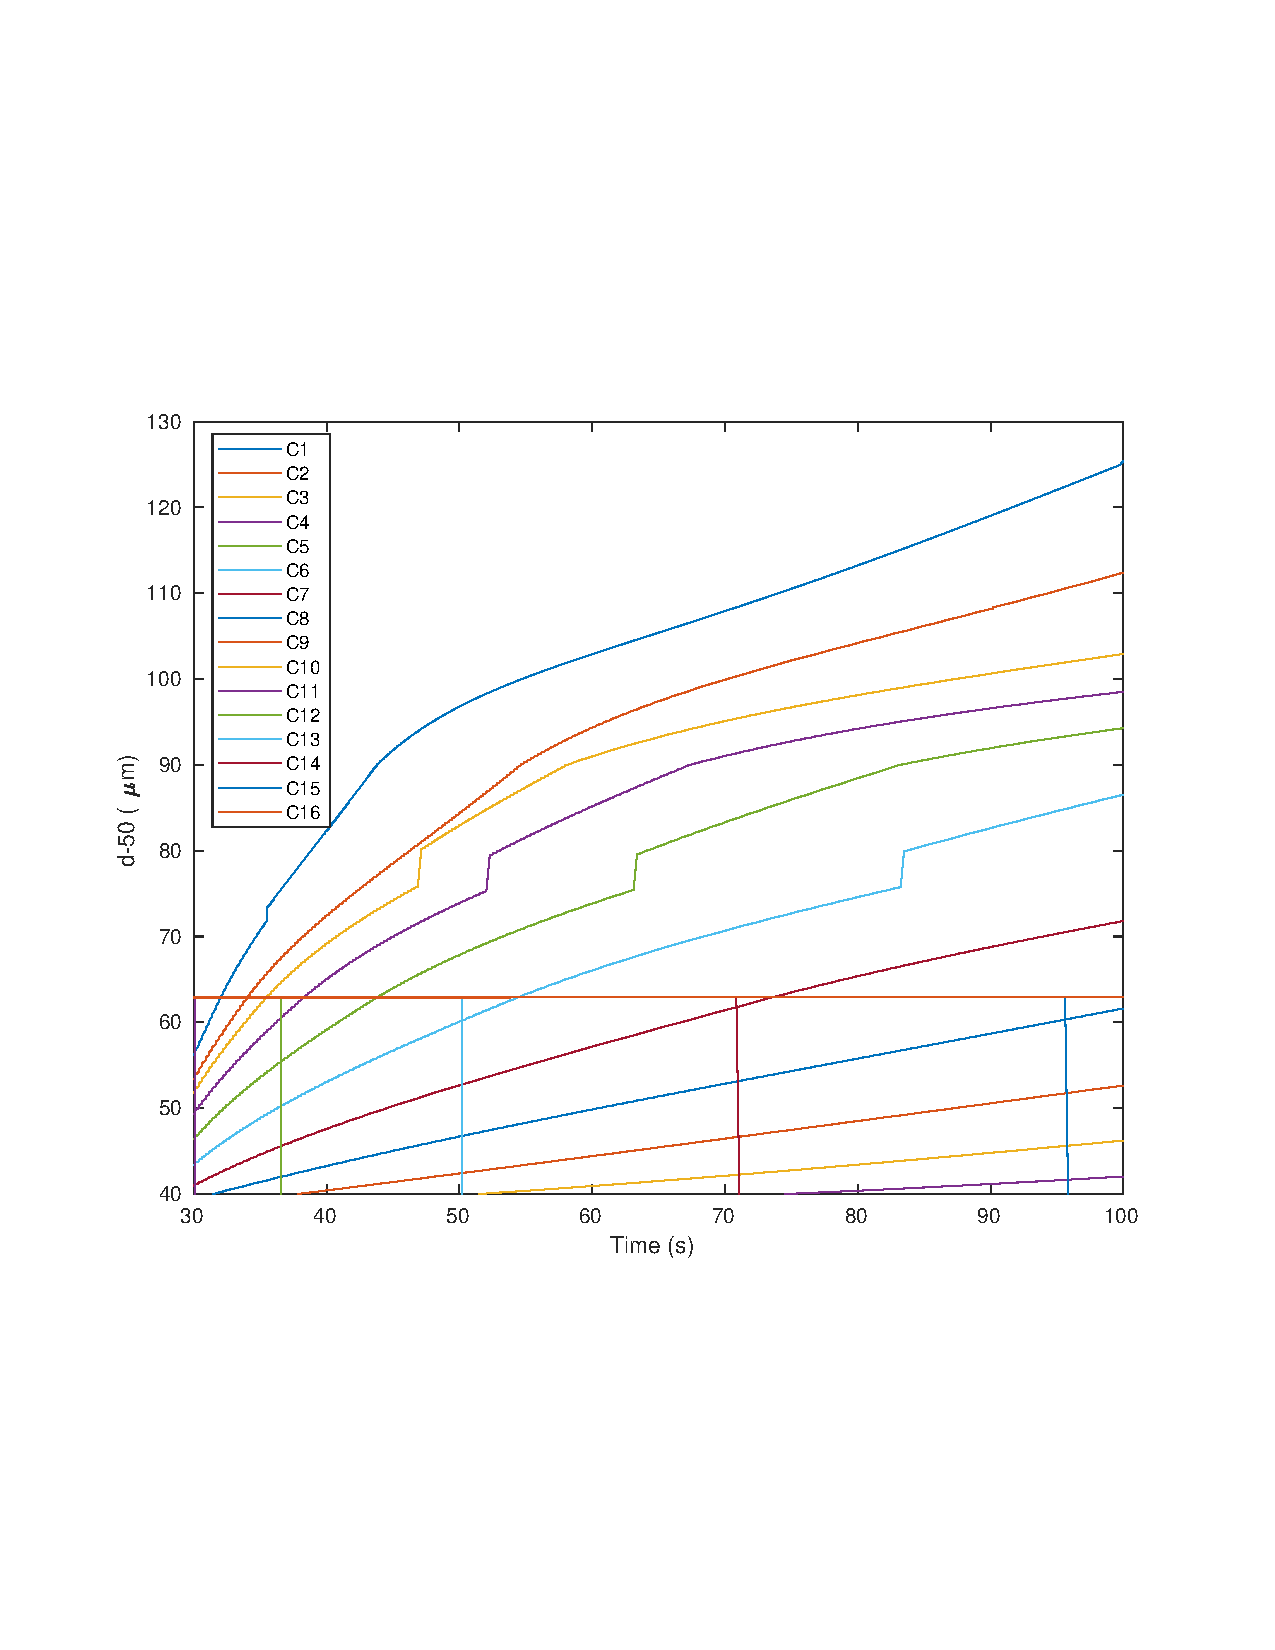
\includegraphics[scale=0.5]{rslts_pbm_d50_128_555.pdf}
\caption{d\textsubscript{50} plot after running the PBM for 100s for the distributed particle size DEM 
simulation. The trend observed is very similar to the trend found in Figure \ref{fig:rslts_PBM_2mm_d50}}
\label{fig:rslts_PBM_psd_d50}
\end{figure}


\subsection{One-way coupled DEM+PBM using RADICAL-Pilot} 
 The RADICAL pilot (RP) being a pilot job system it can bypass the need of waiting on the long scheduler
queues on a cluster. With resources allocated to itself the pilot can execute multiple simulation runs 
at once. The pilot job initiates the DEM simulation using the LIGGGHTS executable compiled for the DEM
studies and then creates a link between the collision data obtained, which is utilized by then utilized 
by the PBM executable. After the link is established, it also initiates the PBM. The timing profiles and
results from both the simulations are then obtained. Since the executables and inputs files used in the 
simulations and the RP job are the similar, we do not expect to see any changes in the physics of the 
system, which is confirmed from the plots of the ratio of the rate of formation to the rate of depletion 
due to aggregation in Figure \ref{fig:rslts_RP_ratio_plot}
\begin{figure}[H]
\centering
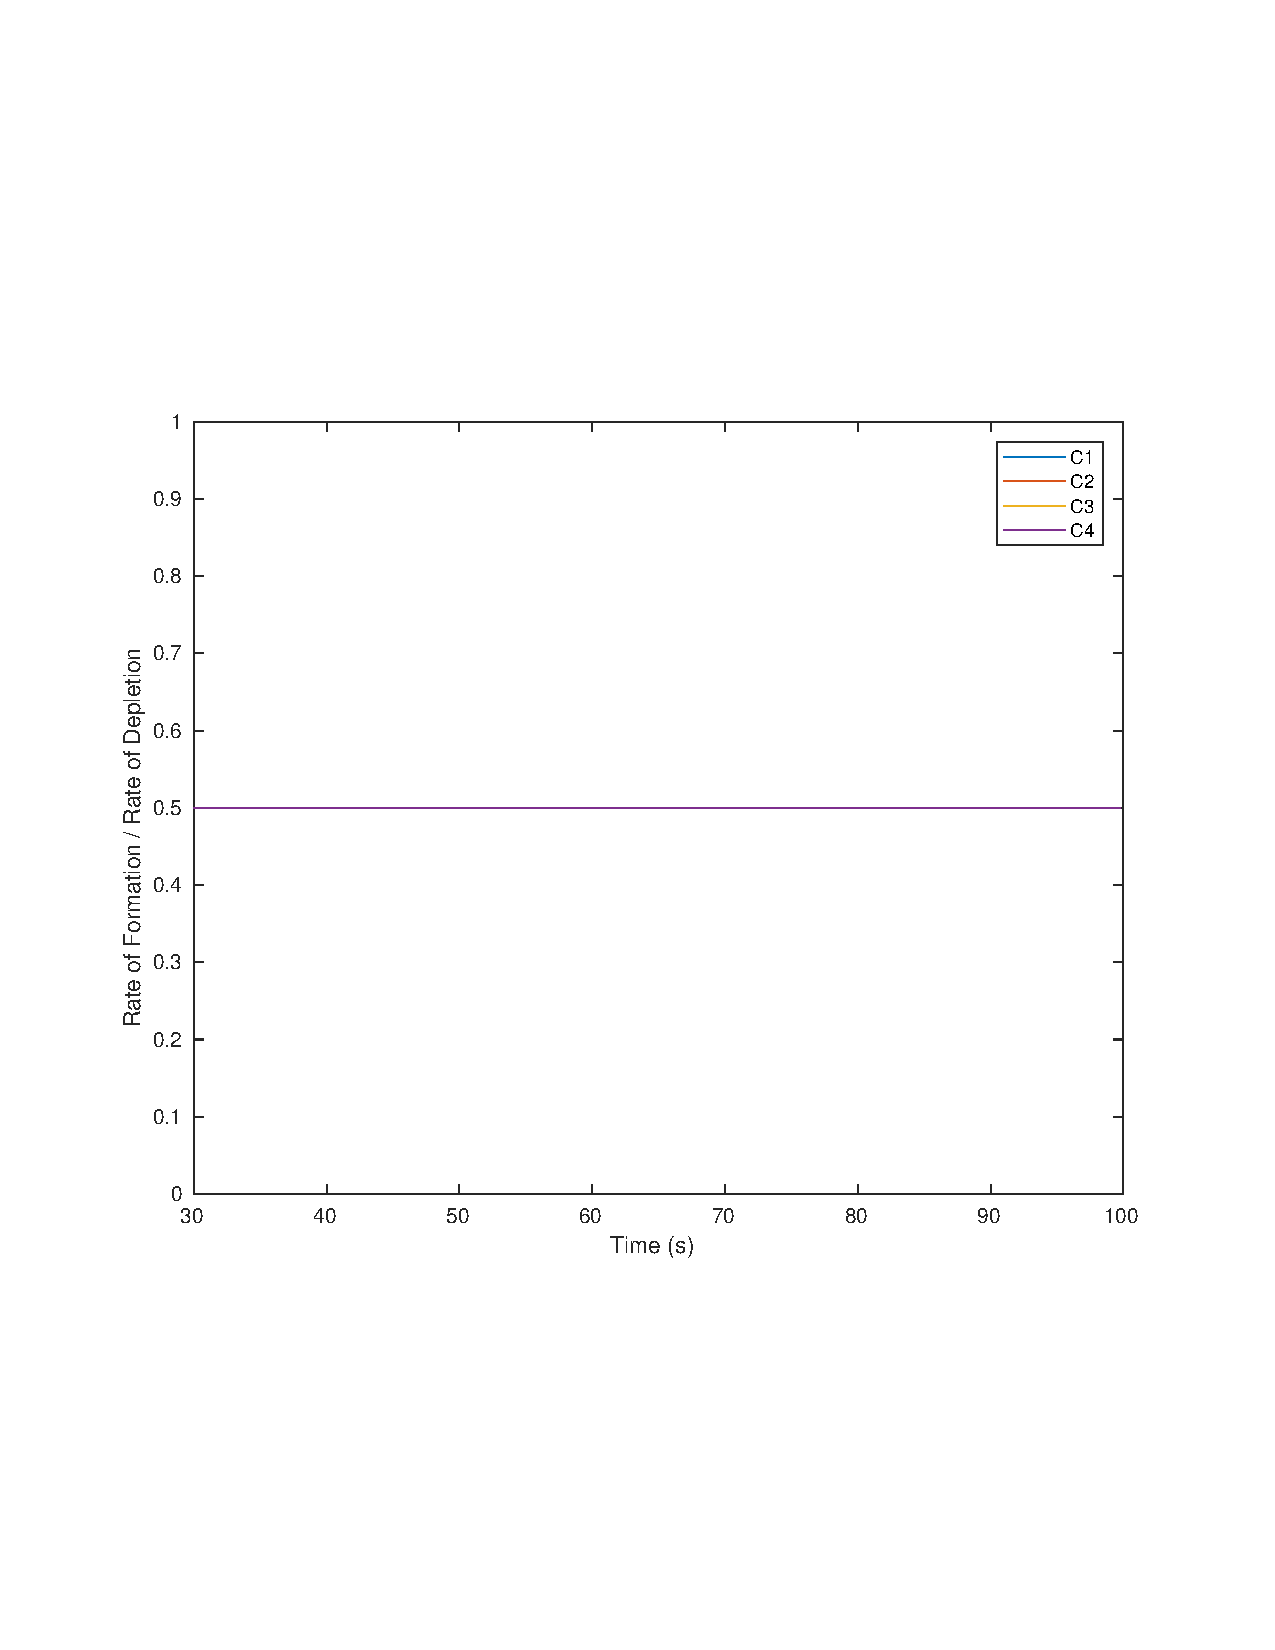
\includegraphics[scale=0.5]{rslts_PBM_2mm_validation.pdf}
\caption{The ratio of rate of formation to the rate of depletion due to aggregation 
as a function of time. Since the ratio is 0.5 as expected, we can say the physics does not change. 
(\textbf{Currently a placeholder})}
\label{fig:rslts_RP_ratio_plot}
\end{figure}

\subsubsection{RADICAL-Pilot performance}
 Since the platforms used for initial development and testing of the DEM and PBM respectively were different, 
the DEM simulations were executed again on Stampede2 for a fair and accurate comparison. The need for re-running
the simulations arises due to the clock speeds of the nodes and their configuration for the 2 platforms is different.
The RADICAL-pilot was setup for Stampede2 and aforementioned experiments were replicated. The DEM simulations were 
run for 64, 128 and 256 cores (MPI processes) and the PBM was run for 1, 2, 4, 8 and 16 MPI processes. No OMP threads 
were implemented for the PBM run, since the current version of RP does not support threading. 
 The times for the individual DEM and PBM simulations were added to determine the total amount time taken to 
simulate the one-way coupling. This time did not include the time spent by each executable in the queue of the 
scheduler. This time could vary from a few hours to a few days depending upon the load of the cluster. The total 
time taken for the simulation using the RADICAL-pilot was determined from the time the DEM was first executed until 
the PBM execution completed. Figure \ref{fig:rslts_RP_time_plot} shows a comparison of the total times of simulation 
for the DEM and PBM individual simulations to the simulation obtained using RP. It can be observed that the times taken 
by the pilot job are slightly higher than the summation of times of the individual simulations. The slight increase in 
the times of the simulation can be accounted to the communication required for the pilot realize that the DEM simulation 
has completed and link the data from the DEM to the PBM executable before it is executable. But, this communication is 
lower than the amount of time the executable the job would spend in the scheduler. Thus, the benefits of using RP become 
clear. An extension of this work would be to use RP to schedule multiple such coupled simulations as one job, thus 
decreasing the wait times even further. 
\begin{figure}[H]
\centering
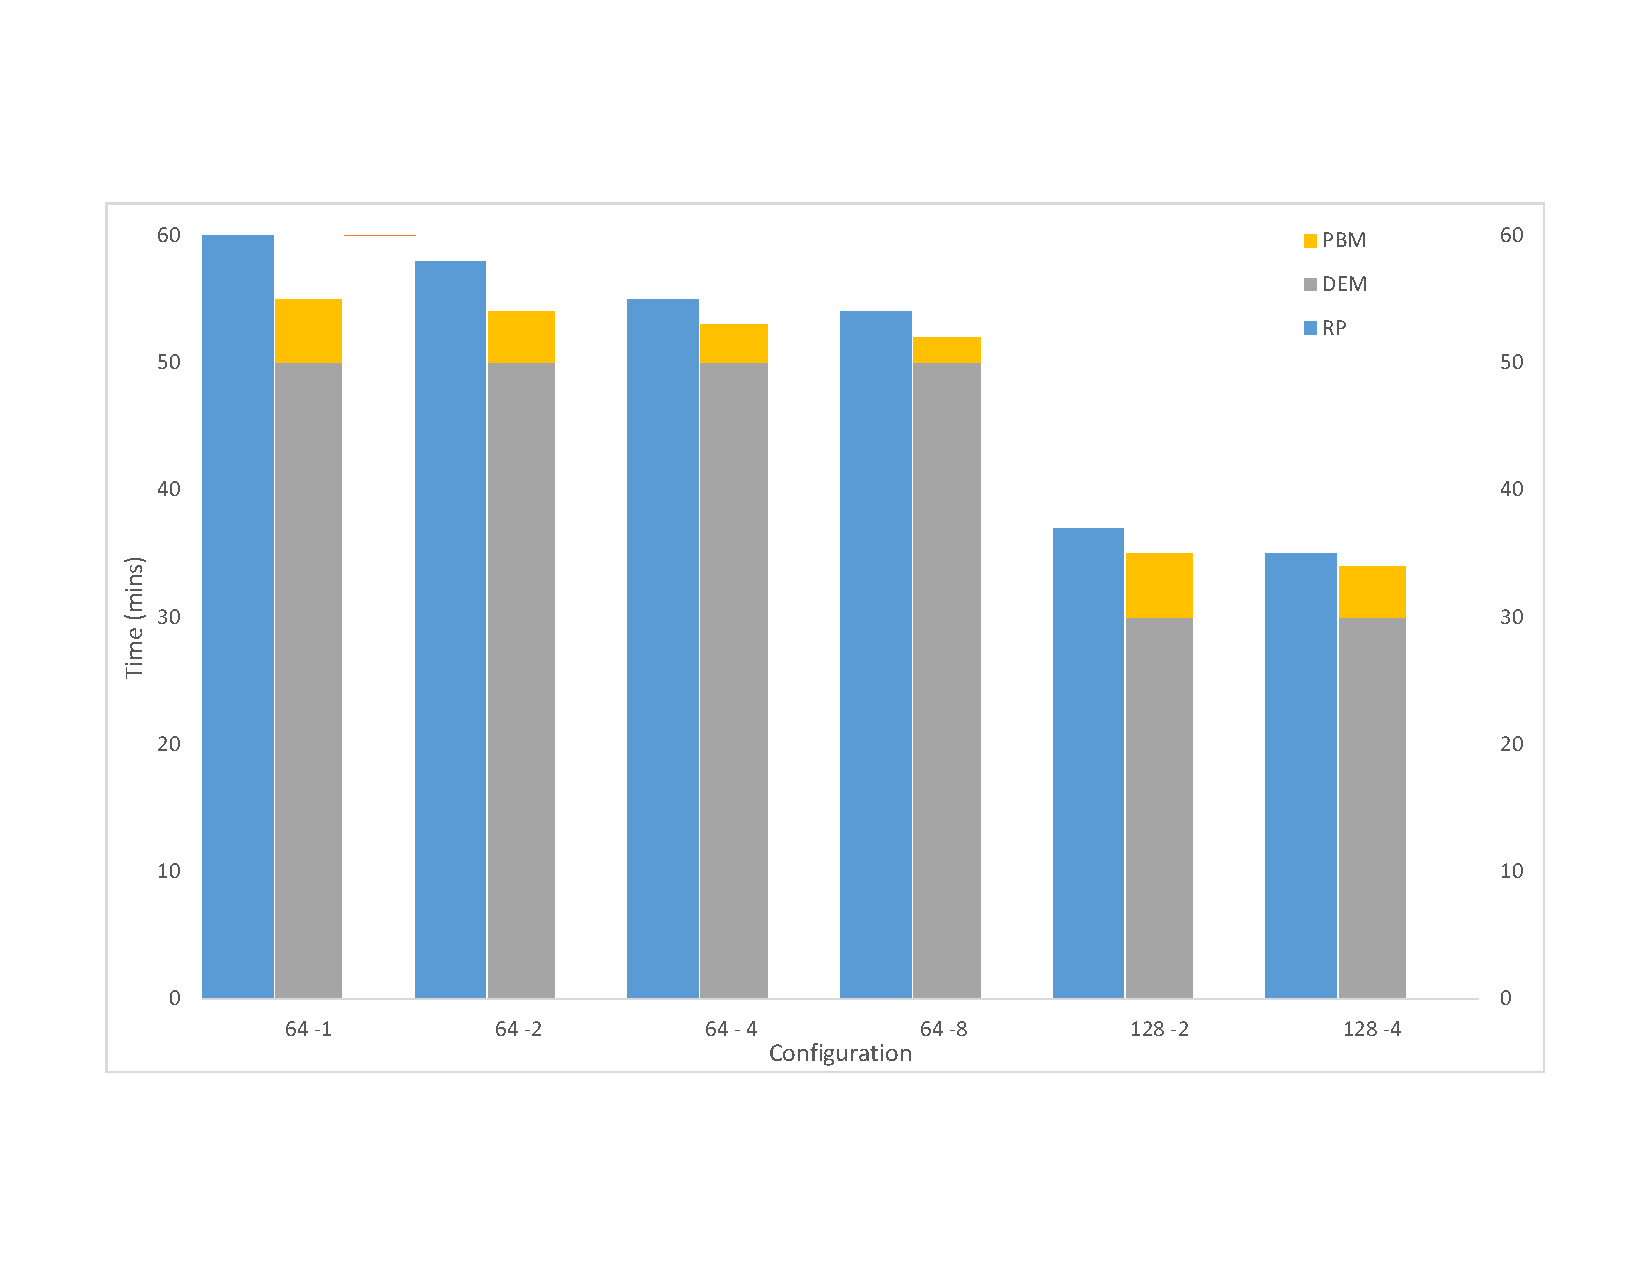
\includegraphics[scale=0.5]{rslts_RP_fake_plot.pdf}
\caption{A comparison of times taken my 2 individual simulations (without adding queue time) v/s time taken by RP. 
(\textbf{Currently a placeholder})}
\label{fig:rslts_RP_time_plot}
\end{figure}
	    
\section{Conclusions}
 A simple uni-directional DEM+PBM coupled study for a high shear granulator has been presented. DEM simulations were 
used to determine the movement of the particles inside the granulator and to obtain the collision data. This collision data 
was then used in the multi-dimensional PBM which was developed with 2 solid bins. Both these executables were parallelized 
to help them utilize the multi-core hardware of a cluster. The DEM was parallelized using MPI where as the developed PBM used 
MPI as well as OMP for a faster execution. The speed-up achieved for the DEM simulation was about 12 times using 64 cores, 
where as the PBM achieved a speed-up of 14 times when 16 cores were used. RP was utilized to execute the simulations for lower 
wait times.
 A more accurate model for the high shear granulator would be to couple the DEM and PBM bi-directionally i.e. these 
two methods are executed iteratively up till a steady state is reached. For the two-way coupling, the computation resources 
required would be really large as it would involve multiple DEM simulations. The role RP in such a situation would more crucial 
as the communication required would increase and it would help reduce total time taken to complete the multiple runs required. 

\section*{References} 
\bibliographystyle{elsarticle-harv}
\bibliography{Bibli}
\end{document}
